\chapter{Análise Bibliográfica sobre Simulações e experimentos voltados para o dilema do prisioneiro iterativo, por João Victor de Souza Calassio\label{chap:bibliometria:jhcf}}

\section{Planejamento do estudo\label{PD@jvcalassio:questoes}}
O planejamento o  desenho do estudo deve descrever as motivações, questões de interesse, escopo, limitações e objetivos do trabalho.

O planejamento do estudo deve motivar o tema escolhido e o interesse do autor.

No caso do meu trabalho, as perguntas que o nortearam foram:
\begin{itemize}
    \item Qual a base de conhecimentos científicos produzida em torno do tema dilema do prisioneiro iterativo, principalmente utilizando simulações? 
    \item Como o dilema do prisioneiro iterativo (e simulações dele) tem sido usado para compreender fenômenos sociais? 
    \item Quais os principais termos e conceitos ligados à frente de pesquisa no tema dilema do prisioneiro iterativo? 
    \item Qual a estrutura social da comunidade, se é que existe, que pesquisa sobre o tema dilema do prisioneiro iterativo?
\end{itemize}

\subsection{O que já existe de pesquisa bibliométrica sobre esse tema?}

O dilema do prisioneiro \cite{noauthor_prisoners_nodate} é um problema conhecido no ramo de teoria dos jogos, e representa uma situação em que dois agentes racionais incomunicáveis entre si devem tomar a decisão de cooperar com o seu parceiro, e ambos compartilharem uma recompensa, ou trair o seu parceiro e ganhar uma recompensa sozinhos, sob o risco de ambos perderem se forem traídos. A versão iterativa consiste na tomada de decisão várias vezes seguidas, lembrando as ações e acontecimentos das vezes anteriores e mudando sua estratégia de acordo com isso.

Modelos como esse têm sido utilizados nas mais diversas áreas da ciência, como na economia, política e até mesmo ecologia \cite{almeida_equilibrio_2012}.

\subsection{Uso do Bibliometrix e Biblioshiny}
Serão usadas a ferramenta e o \textit{workflow} proposto pelos autores do pacote Bibliometrix, conforme indica a figura ~\ref{fig:bibliometrix:workflow}.

\subsection{Limitações} O exercício relatado foi feito em 5 dias, envolvendo entre 6 a 10 horas de trabalho de cada autor.

Outros aspectos a reforçar:
\begin{itemize}
   
\item Deve-se fazer buscas na base de dados WoS ou SCOPUS;
\item é obrigatório declarar um conjunto de perguntas de pesquisa.
\item é preciso declarar o objetivo da pesquisa, que no caso da aqui relatada foi exercitar inicialmente, e relatar, o uso da técnica de análise bibliométrica, para fins didáticos.
\end{itemize}


\section{Coleta de dados\label{PD@jvcalassio:coleta}}

A coleta de dados feita usando o WoS no dia 01 de dezembro de 2022, acessado por meio do Portal de Periódicos da CAPES.

\subsection{Query de Busca}

Foi usada a \query\  de busca ilustrada nas linhas 1 a 6 da listagem \ref{PD@jvcalassio:querylst}.

\lstinputlisting[numbers=left,basicstyle=\normalsize\ttfamily,caption={\query\  de busca sobre dilema do prisioneiro iterativo.},label=PD@jvcalassio:querylst]
{exploratory-data-analysis/jvcalassio/PesqBibliogr/PrisonersDilemma/WoS-20221201/query.txt}

\subsubsection{Explicação para os termos de busca usados\label{PD@jvcalassio:query}}

A busca consistiu de três cláusulas disjuntivas, unidas por uma conjunção \textit{and}, aplicadas à busca por tópico (O termo de busca pode aparecer no Título, no Abstract, nas Author Keywords, ou nas Keywords Plus da referência)

Os termos \texttt{iterat*}, \texttt{recurrent}, \texttt{repeat*} e \texttt{repetitive}
foram utilizadas na primeira cláusula da consulta para recuperar artigos que tratem específicamente do
dilema do prisioneiro iterativo.

Os termos \texttt{prisoner*} e \texttt{dilemma} foram utilizados na segunda e terceira cláusulas para recuperar os artigos que tratem sobre o dilema do prisioneiro.

Pesquisas com os termos \texttt{simul*} e \texttt{spatial} retornaram muitos poucos resultados (menos de 500) e por isso não foram utilizados.

\subsection{Registros recuperados}

Os 1.860 registros obtidos como resultado da busca encontram-se em \url{https://github.com/jhcf/Comput-Experim-20222/blob/main/exploratory-data-analysis/jvcalassio/PesqBibliogr/PrisonersDilemma/WoS-20221201/1860records.txt}. 

Foram utilizadas as opções \textit{Exportar registros para arquivo de texto sem formatação} e \textit{export full record / Gravar Conteúdo: Seleção personalizada, com todos os 29 campos disponíveis, inclusive referências citadas} no WoS, para que as citações também fosse usadas em análises da citações (estrutura intelectual do conhecimento). Os 1.860 registros foram recuperados em duas exportações, uma com os registros de 1 a 1.000, e outra com os registros de 1.001 a 1.860.

A listagem \ref{PD@jvcalassio:sample} apresenta as 59 linhas de um registro no formato RIS, referentes a um artigo recuperado da Web of Science. Cada um dos campos de um registro é marcado por um código de dois caracteres, nas colunas 1 e 2 de cada linha. Se a coluna está em branco repete-se o mesmo campo da linha anterior.
O significado de cada campo pode ser visto em \citep{wikipedia_ris_2017}.

Alguns campos específicos serão comentados a seguir:
\begin{description}
    \item [PT - Publication Type] indica o tipo da publicação, no caso específico um artigo de \textit{journal} (J);
    \item [AU - Author] Nome de um autor;
    \item [AF - Author Full Name] Nome completo de um autor;
    \item [TI - Title] Título da publicação;
    \item [SO - Source] Nome da revista;
    \item [DE - Descriptor] Palavras-chave;
    \item [AB - Abstract] Resumo;
    \item [CR - Cited Referente] Cada uma das referências citadas no artigo;
    \item [TC - Times Cited] Quantidade de vezes que esse artigo foi globalmente citado;
    \item [PY - Publication Year] Ano de publicação;
    \item [VL - Volume, IS - Issue] Volume e número onde o artigo foi publicado, na revista;
    \item [BP - Begin page, EP - End page] Páginas inicial e final do artigo dentro do volume e número da revista;
    \item [DI - Digital Object Identifier] Identificador único do artigo no sistema \url{http://doi.org};
    \item [DA - Date of Acquisition] Data em que o registro foi obtido da WoS;
    \item [ER - End of Record] Fim do registro.
\end{description}

\lstinputlisting[numbers=left,basicstyle=\tiny\ttfamily,caption={Exemplo de um registro recuperado no formato RIS, sobre o tema dilema do prisioneiro iterativo.},label=PD@jvcalassio:sample]
{exploratory-data-analysis/jvcalassio/PesqBibliogr/PrisonersDilemma/sample.txt}

\section{Análise dos dados\label{PD@jvcalassio:analise}}

\subsection{Filtragem de registros}
Antes da análise, é possível aplicar filtros sobre os registros obtidos.

Foi aplicado um filtro ao \dataset\   inicial, com 1.860 registros, que continham pŕevias de artigos, artigos de conferência, capítulos de livro etc. Foram mantidos apenas os registros de artigos publicados em revistas científicas\footnote{A suposição é que que o conhecimento de maior qualidade sobre o tema está nas publicações em revistas.}. Após a aplicação desse filtro, 1.387 registros foram mantidos no \dataset, que será doravante chamado PD, ou PD@jvcalassio.

\subsection{Análise descritiva do \dataset\   PD@jvcalassio}

A análise bibliométrica descritiva faz uma descrição inicial do \dataset\  . Para explicação detalhada de como são calculadas as diversas taxas geradas pelo Bibliometrix veja a documentação do \textit{package} a partir da página \url{https://cran.r-project.org/web/packages/bibliometrix/index.html}. A análise bibliométrica descritiva é gerada pela função \texttt{biblioAnalysis}.

As informações mais gerais sobre o \dataset\   PD@jvcalassio são as seguintes:
\begin{description}
    \item [\textit{Timespan}] Os artigos que atenderam aos critérios de busca e filtragem foram publicados a partir de 1966, até 2022. Até 1992, eram publicados poucos artigos sobre o tema.
    \item [\textit{Sources (Journals, Books, etc)}] São 451 fontes de informação que publicaram os documentos recuperados no \dataset\   PD@jvcalassio. Ou seja, em média, cada \textit{scientific journal} publicou $1.387/451=3,07$ artigos. \footnote{Note que a média, enquanto medida de tendência central, pode não ser a que melhor reflete a tendência a quantidade de artigos publicados por revista.}
    \item [\textit{Document average age}] A média do tempo de publicação dos artigos no \dataset\   PD@jvcalassio é de 12,1 anos.
    \item [\textit{Average citations per documents}] Cada artigo no \dataset\   PD@jvcalassio foi citado, em média 32,99 vezes\footnote{Note que a média, enquanto medida de tendência central, pode não ser a que melhor reflete a tendência de  citações a artigos.}.
    % \item [\textit{Average citations per year per doc}] Após publicado, cada um dos 5.787 artigos do \dataset\   MASSA@jhcf  foi citado 2,262 vezes por ano, em média.
    \item [\textit{References}] O \dataset\   PD@jvcalassio contém 26.106 referências citadas (tags CR).
    \item [\textit{Keywords Plus (ID)}] 1.551 distintas palavras-chave do tipo Keywords Plus (ID)\footnote{\textit{KeyWords Plus} são ``termos de índice gerados automaticamente a partir dos títulos de artigos citados. Os termos do KeyWords Plus devem aparecer mais de uma vez na bibliografia e são ordenados de frases com várias palavras a termos únicos. O KeyWords Plus aumenta o número de resultados tradicional de palavras-chave ou títulos.'' Fonte: \url{https://images.webofknowledge.com/WOKRS410B4/help/pt_BR/WOS/hp_full_record.html}} foram encontradas no \dataset\   PD@jvcalassio. 
    \item [\textit{Author's Keywords (DE)}] 2.181 distintas palavras-chave indicadas pelos autores foram encontradas no \dataset\  PD@jvcalassio.
    \item [\textit{Authors}] 2.353 distintos nomes de autores foram encontrados no \dataset\ PD@jvcalassio. \footnote{Um mesmo autor pode ter uma ou mais diferentes grafias no \dataset\  , e serão reconhecidos dois ou mais autores diferentes, embora de fato sejam apenas um. Isso significa que a quantidade de \textbf{nomes de autores} equivale à quantidade de \textbf{autores}. Adicionalmente, é possível que distintos autores sejam reconhecidos com o mesmo nome, isso é, que sejam homônimos. Ou seja, o \dataset\   em geral conterá erros de contagem na quantidade de autores reais.}.
    % \item [\textit{Author Appearances}] Os 19.410 distintos (nomes de) autores foram encontrados 23.470 vezes, como autores de artigos.
    \item [\textit{Authors of single-authored documents}] Dentre os 2.353 distintos (nomes de) autores encontrados, 290 deles editaram artigos individualmente, isso é, sem co-autores.
    % \item [\textit{Authors of multi-authored documents}] Dentre os 19.410 distintos (nomes de) autores encontrados, 19.035 deles editaram artigos com um ou mais co-autores"
    \item [\textit{Single-authored documents}] Dentre os 1.387 documentos presentes no \dataset\   PD@jvcalassio, 358 foram escritos por um único autor, e os 1.029 restantes foram elaborados em co-autoria.
    % \item [\textit{Documents per Author}] Dentre os 19.410 distintos (nomes de) autores, cada um publicou em média 0,298 artigos.
    \item [\textit{Authors per Document}] Cada um dos 1.387 documentos presentes no \dataset\   PD@jvcalassio foi autorado com 1,69 autores em média ($2.353 / 1.387 = 1,69$).
    \item [\textit{Co-Authors per Documents}] As aparições de (nomes de) autores (``Author Appearances''), se distribuem, em média 2,45 vezes para os 1.387 documentos do \dataset\   PD@jvcalassio.
    % \item [\textit{Collaboration Index}] Os 19.035 (nomes de) autores que editaram artigos com um ou mais co-autores, colaboraram em media 3,54 vezes para editar os 5.378 artigos elaborados em co-autoria, gerando, assim, um índice de colaboração 3,54. 
\end{description}



\subsection{Evolução da Produção Científica}

\begin{figure}
    \centering
    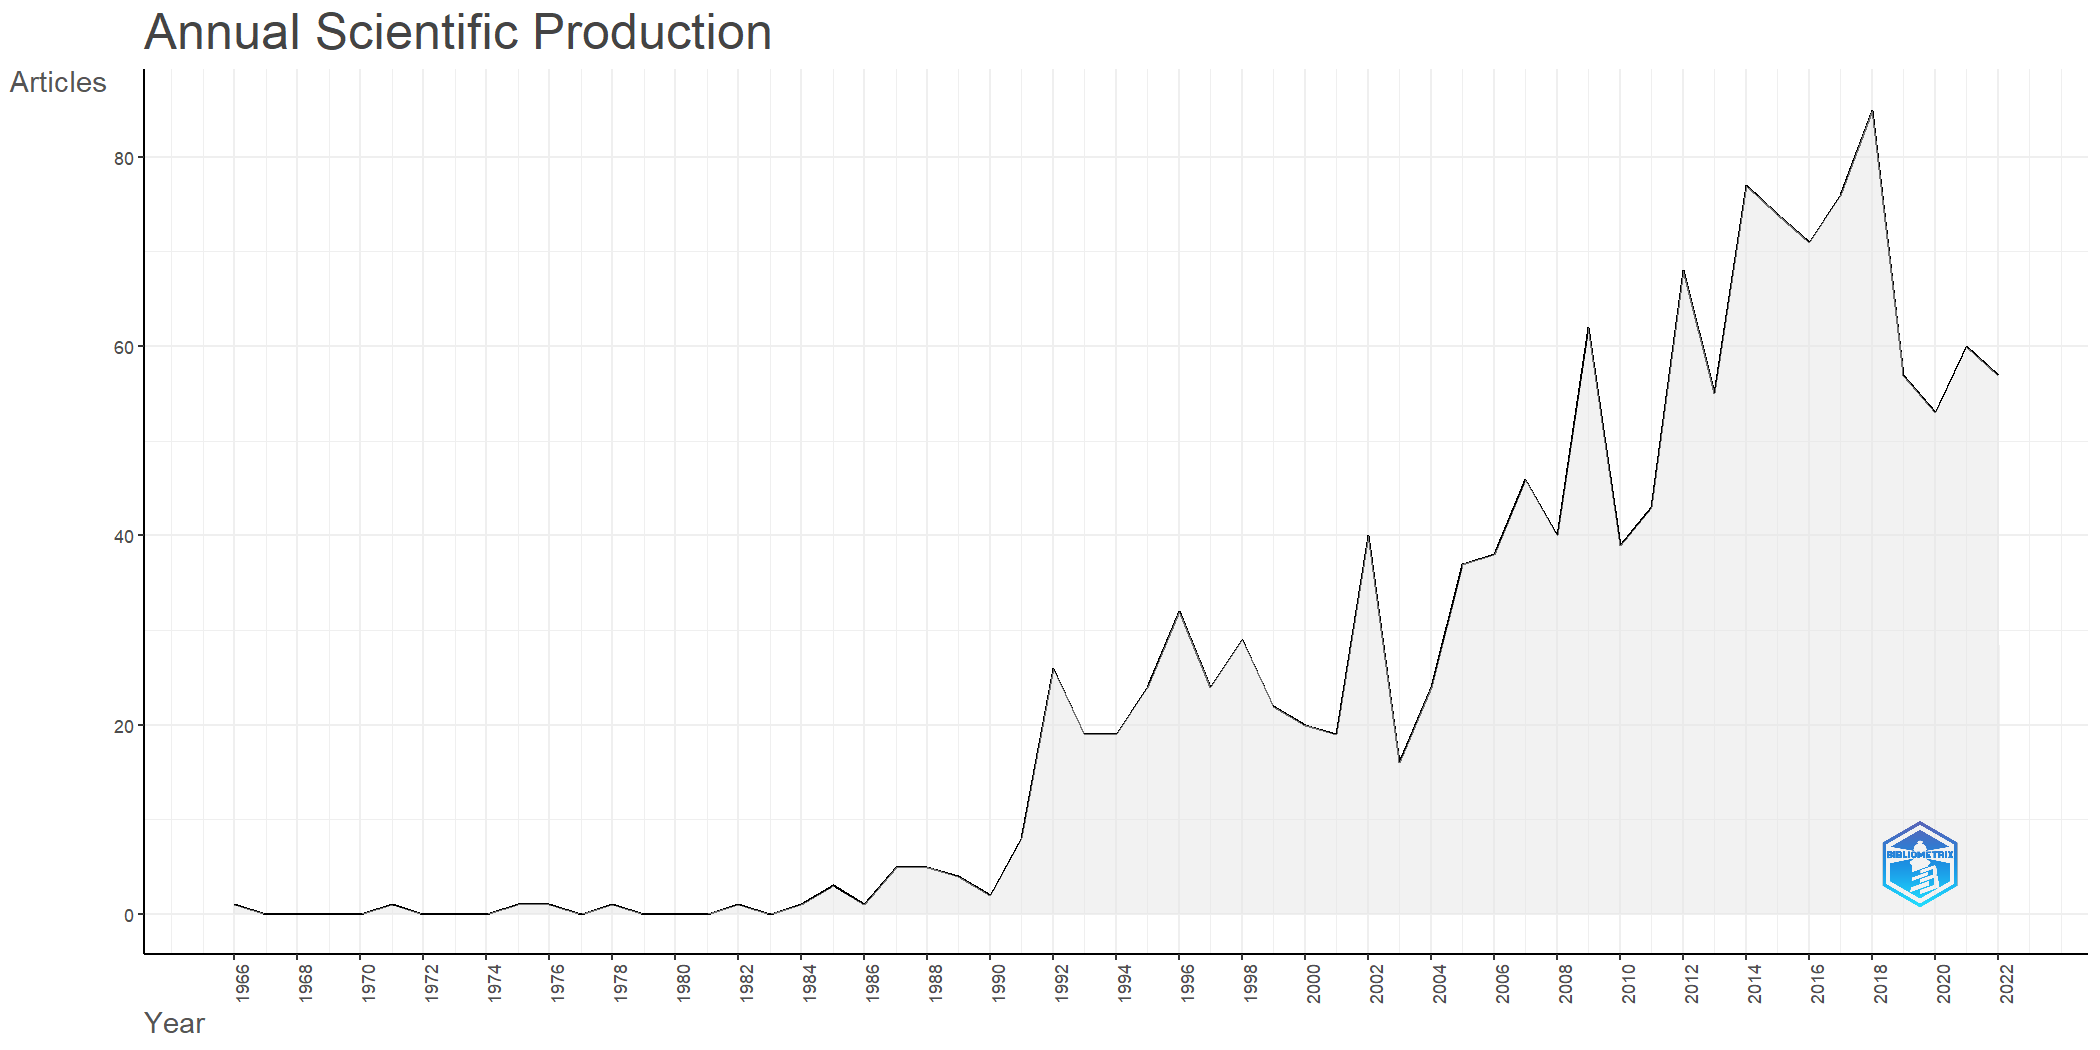
\includegraphics[width=1\textwidth]{exploratory-data-analysis/jvcalassio/PesqBibliogr/PrisonersDilemma/WoS-20221201/Dataset/AnnualScientificProduction-2022-12-01.png}
    \caption{Evolução da produção científica no \dataset\   PD@jvcalassio.}
    \label{fig:evol:anual:PD@jvcalassio}
\end{figure}

A figura \ref{fig:evol:anual:PD@jvcalassio} apresenta a evolução da produção científica mundial no tema de interesse, segundo o \dataset\   PD@jvcalassio. A curva mostra que desde a primeira publicação, em 1966 até 1991 foram publicadas poucos artigos que tratam desse tema. A partir de 1992, apareceu uma tendência de crescimento da quantidade de publicações, provavelmente graças à publicação de \citet{poundstone_prisoners_1992}.

O \textit{Annual Growth Rate} do \dataset\   é de 7,49\%, consideravelmente maior que a taxa média de crescimento da publicação científica mundial, de cerca de 3,3\% anuais, em 2016, como ilustra o estudo em \url{https://www.researchgate.net/publication/333972683_Dynamics_of_scientific_production_in_the_world_in_Europe_and_in_France_2000-2016}, página 23.

\subsection{Interpretação do Crescimento} A maior taxa de crescimento do \dataset\   PD@jvcalassio, bem como o seu grande volume, sugerem que o assunto em pauta desperta intenso interesse, inclusive de ordem econômica.

\subsection{Evolução das Citações}

\begin{figure}
    \centering
    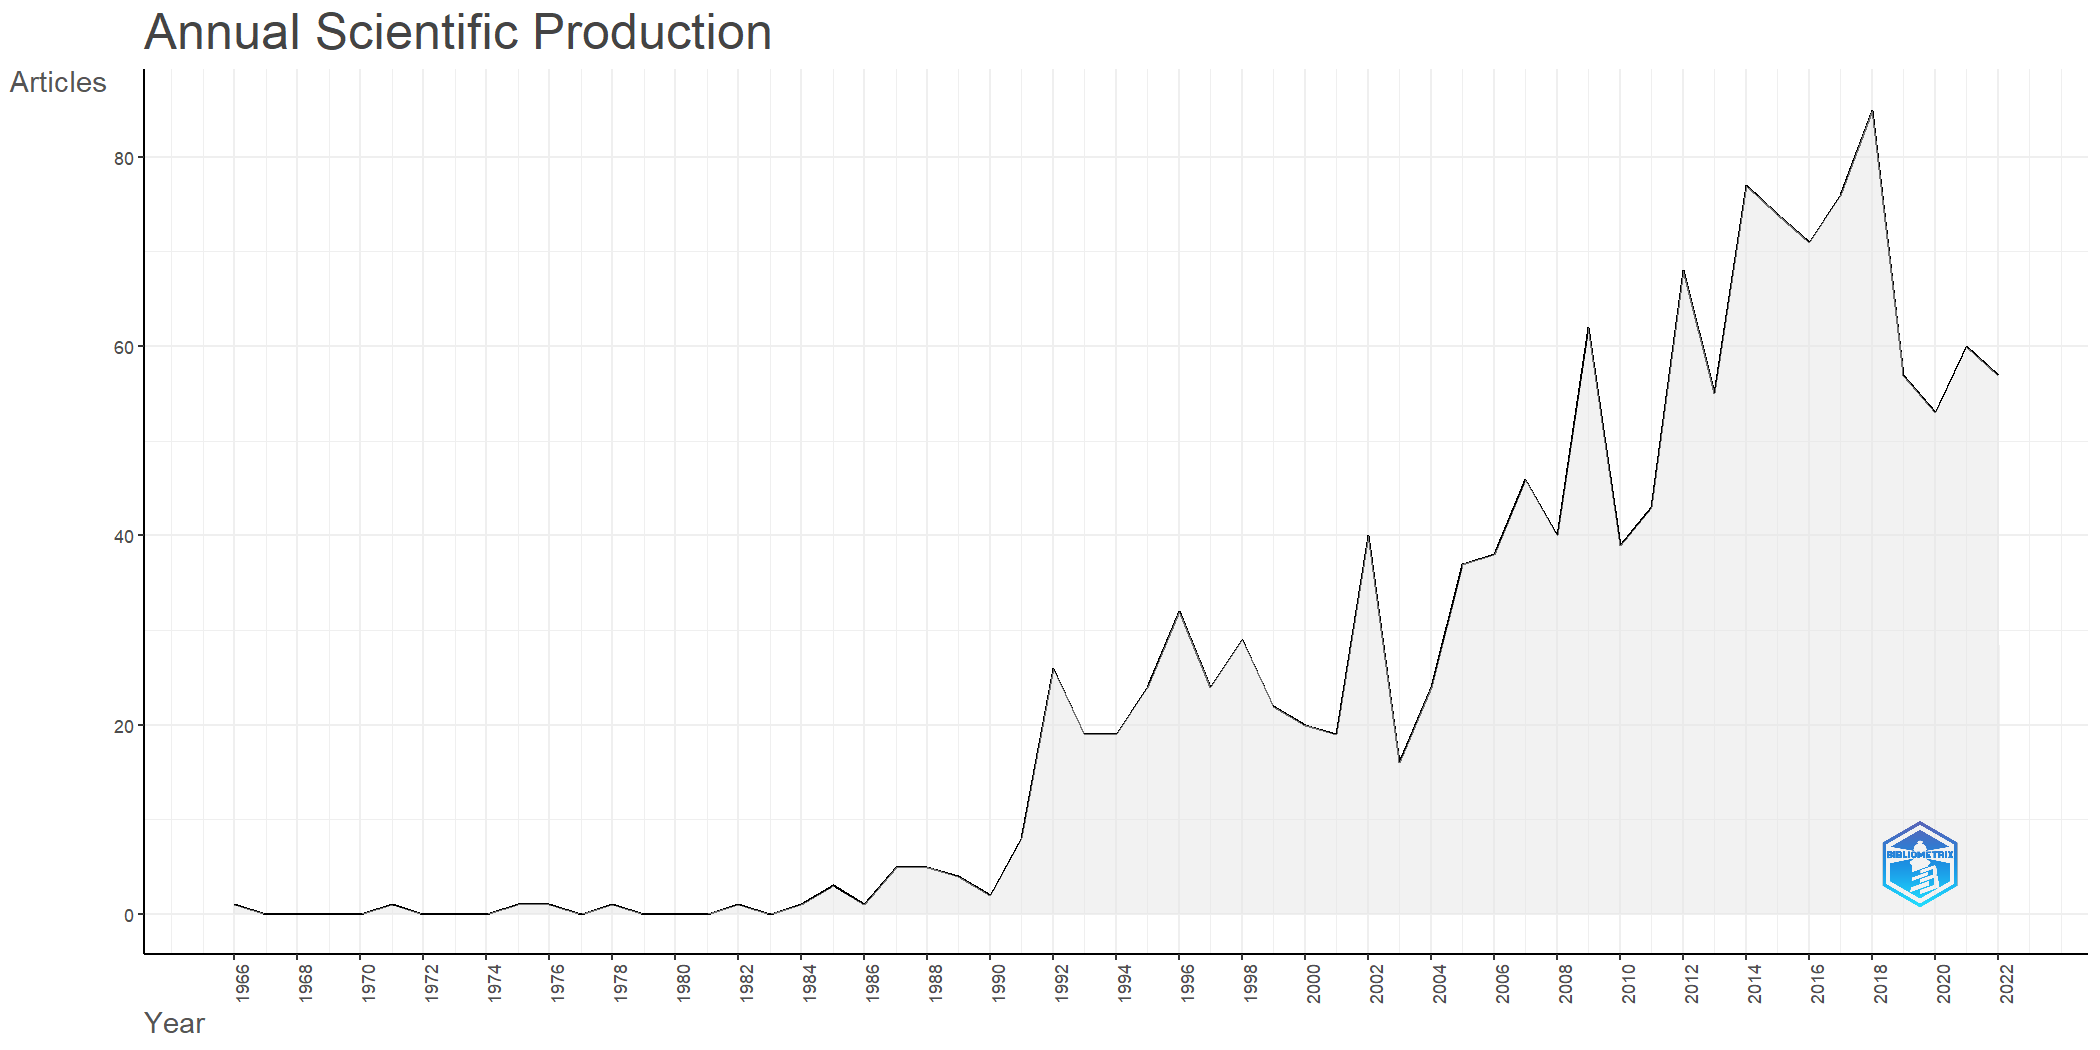
\includegraphics[width=1\textwidth]{exploratory-data-analysis/jvcalassio/PesqBibliogr/PrisonersDilemma/WoS-20221201/Dataset/AnnualScientificProduction-2022-12-01.png}
    \caption{Evolução das citações ao \dataset\   PD@jvcalassio.}
    \label{fig:evol:anual:citacoes:PD@jvcalassio}
    
\end{figure}

A figura \ref{fig:evol:anual:citacoes:PD@jvcalassio} apresenta a evolução da média de citações aos 1.387 artigos no \dataset\   PD@jvcalassio.

A média anual de citações é relativamente estável, se mantendo entre 0 e 10 de 1966 até 2022. Há um pico em 1982, com 27,82 citações.

\footnote{Note que o cálculo do número  médio de citações, nesse caso, utiliza os valores computados no tag "TC (Times Cited)", já presentes no \dataset\   obtido. Ou seja, o gráfico baseia-se no número de citações globais (externas ao \dataset\   PD@jvcalassio), e não no número de citações locais (citações a um artigo do \dataset\   feitas por alguns dos outros artigos dentro do próprio \dataset).}

\subsection{Interpretação das Citações}
Mesmo com o crescimento anual (em média) no número de publicações, a média de citações continua em um número consideravelmente estável. Isso quer dizer que esses artigos continuam mantendo sua relevância, e são cada vez mais citados por outros artigos e despertam interesse em outras áreas do conhecimento.

\subsection{\textit{Three-Field Plots (Sankey diagram)} \label{PD@jvcalassio:Sankey}}

As \textit{Three-Field Plots (Sankey diagram)} (plotagens do tipo ``Três Campos'') apresentam afinidades entre três conjuntos de atributos agregados que ocorrem no \dataset. Uma plotagem do tipo Sankey busca mostrar os principais fluxos entre diferentes conjuntos de\lstinputlisting[numbers=left,basicstyle=\normalsize\ttfamily,caption={\query\  de busca sobre simulação multiagente de fenômenos socials, com ênfase em métodos experimentais.},label=query20210803-2]
{exploratory-data-analysis/jhcf/PesqBibliogr/SimulacaoMultiagente/WoS-20210803/classico-mais-citacoes/query.txt} itens. \footnote{Para uma introdução ver \url{https://en.wikipedia.org/wiki/Sankey_diagram}. Para obter detalhes sobre a forma de geração e utilização desse gráfico, inclusive de forma interativa, veja o vídeo em \url{https://www.youtube.com/watch?v=jBb1iha6-sg}.} 

\begin{figure}
    \centering
    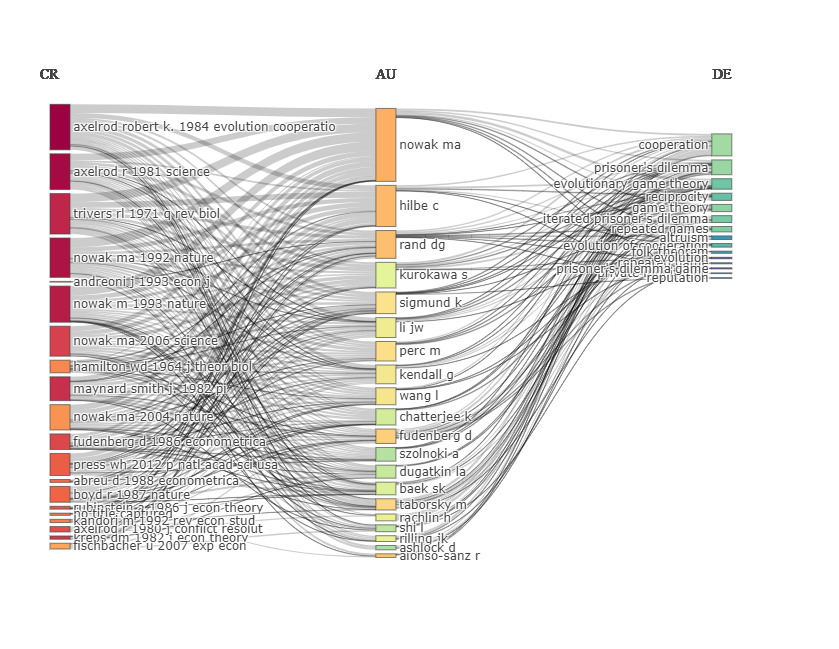
\includegraphics[angle=0,width=1\textwidth]{exploratory-data-analysis/jvcalassio/PesqBibliogr/PrisonersDilemma/WoS-20221201/Dataset/ThreeFieldPlot-2022-12-02.png}
    \caption{Plotagem ``Três Campos'' (Sankey plot) do \dataset\   PD@jvcalassio: 20 Autores, Citações e Palavras-Chave mais proeminentes.}
    \label{fig:PD@jvcalassio:ThreeFieldPlot}
\end{figure}

A figura \ref{fig:PD@jvcalassio:ThreeFieldPlot} apresenta a plotagem do tipo ``Três Campos'' do \dataset\   PD@jvcalassio, vinculando, ao centro, os 20 Autores mais proeminentes (AU), à esquerda, as 20 Citações mais frequentes (CR - Cited Records), e à direita, as 20 Palavras-Chave mais frequentes empregadas pelos autores.

\subsection{Interpretação da figura \ref{fig:PD@jvcalassio:ThreeFieldPlot}}

Dentre as palavras-chave (DE) não relacionadas diretamente aos termos de busca, se destacam \textbf{cooperation}, \textbf{reciprocity}, \textbf{altruism}, \textbf{evolution}, \textbf{evolution of cooperation}. Isso sugere que pesquisas nessa área buscam entender como a cooperação, reciprocidade e altruísmo entre indivíduos evoluem ao longo do tempo em um experimento repetitivo como o dilema do prisioneiro iterativo.

Observa-se também que os artigos mais citados foram publicados em sua maioria na década de 1980, com exceções relevantes em 1992, 1993, 2004 e 2006, todas pelo mesmo autor (NOWAK MA). Isso sugere que não houveram grandes mudanças de paradigma no tema nos últimos 10 anos, e o maior progresso após o trabalho de Robert Axelrod na década de 80 foi através do trabalho de Nowak.

A fim de melhor evidenciar as citações mais relevantes segundo o peso dos autores e palavras-chave, o gráfico da figura \ref{fig:PD@jvcalassio:ThreeFieldPlot:10-20-20} plota apenas as 10 referências citadas, para 20 autores e palavras-chave mais proeminentes.

\begin{figure}
    \centering
    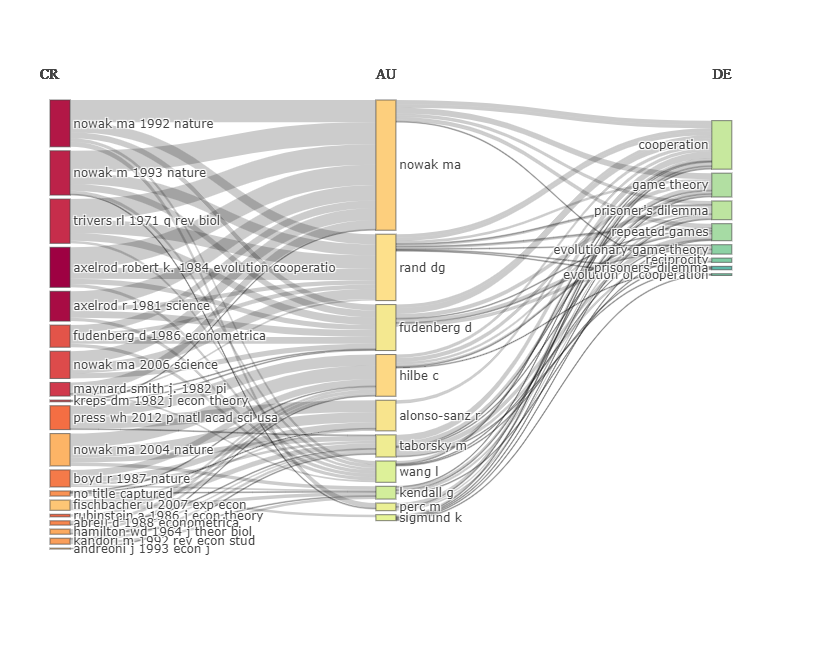
\includegraphics[angle=0,width=1\textwidth]{exploratory-data-analysis/jvcalassio/PesqBibliogr/PrisonersDilemma/WoS-20221201/Dataset/ThreeFieldPlot-102020-2022-12-02.png}
    \caption{Plotagem ``Três Campos'' (Sankey plot) do \dataset\   PD@jvcalassio: 10 Autores, 20 Citações e Palavras-Chave mais proeminentes.}
    \label{fig:PD@jvcalassio:ThreeFieldPlot:10-20-20}
\end{figure}

\subsubsection{Autores mais relevantes\label{PD@jvcalassio:Sankey:AutoresRelevantes}}

Breves comentários sobre cinco dos trabalhos mais citados serão apresentados a seguir.

\begin{itemize}
    \item \cite{axelrod_evolution_1981} apresenta um modelo baseado em uma estratégia evolucionária estável no contexto do dilema do prisioneiro para entender a cooperação entre pares de indivíduos, e mostra como a cooperação baseada na reciprocidade surge em uma sociedade, e como ela pode ser bem sucedida uma vez implantada, através de uma série de torneios realizados por um computador;
    \item \cite{greene_review_1984} apresenta uma análise de \cite{axelrod_evolution_1981};
    \item \cite{nowak_tit_1992} analisa como reações de ``olho-por-olho'' afetam populações heterogêneas em uma situação mais próxima à biológica, e mostra que apenas uma pequena parcela das reações de ``olho-por-olho'' são essenciais para o surgimento da reciprocidade nessas populações;
    \item \cite{nowak_strategy_1993} apresenta uma estratégia (Pavlov, que consiste em continuar se estiver ganhando, e trocar se perder) que é tão simples quanto a ``olho-por-olho'', mas é mais robusta e parece descrever melhor a cooperação em situações naturais;
    \item \cite{trivers_evolution_1971} apresenta um modelo que representa na seleção natural o que é chamado de ``comportamento altruístico recíproco'', e mostra como a seleção natural trabalha contra um indíviduo que não seja reciprocador dentro do sistema;
\end{itemize}

Apenas um dos documentos citados está contido no \dataset\   recuperado.

\subsection{Citações globais aos artigos no \dataset}

Cada registro recuperado no \dataset\ apresenta um conjunto de informações, dentre as quais pode constar a quantidade de vezes que uma citação ao mesmo foi registrada no índice do WoS, desde que no momento da extração seja feita essa solicitação (\textit{TC - Times Cited}).
A tabela \ref{tab:PD@jvcalassio:GlobalCitations} apresenta a lista dos 25 artigos do \dataset, que foram mais citados, ordenados de forma decrescente pelo número global de citações do artigo, nos índices da WoS. Para ada artigo é apresentada a referencia abreviada, o DOI e a quantidade de vezes que ele foi citado globalmente (no índice do WoS). Para recuperar a página do artigo deve-se abrir uma url prefixada com \url{http://doi.org/}, e informar o valor do DOI indicado, por exemplo \url{https://doi.org/10.1038/359826a0} levará à página do artigo mais citado, cujo título é ``Evolutionary games and spatial chaos''.

\begin{table}[htp]
    \footnotesize
    % \csvreader[tabular = |r|l|l|r|,
    % separator=semicolon
    % %,filter not strcmp={\csvcolii}{},
    % , table head = \hline\hline \# & Artigo (Referência Abreviada) & DOI (Digital Object Identifier) & Tot.Cit.\\ \hline\hline,
    % table foot = \hline\hline
    % ]{exploratory-data-analysis/jvcalassio/PesqBibliogr/PrisonersDilemma/WoS-20221201/Dataset/Most-Global-Cited-Documents.csv}{Paper=\paper, DOI=\doi,Total Citations=\totcit}{ \thecsvrow & {\tiny\paper} & {\tiny \doi} & \totcit}
    \resizebox{\textwidth}{!}{\begin{tabular}{|l|l|l|l|l|}
    \hline
        Paper & DOI & Total Citations & TC per Year & Normalized TC \\ \hline
        NOWAK MA, 1992, NATURE-a & 10.1038/359826a0 & 2681 & 86.48 & 11.67 \\ \hline
        NOWAK MA, 1998, NATURE & 10.1038/31225 & 1515 & 60.60 & 17.08 \\ \hline
        KREPS DM, 1982, J ECON THEORY & 10.1016/0022-0531(82)90029-1 & 1115 & 27.20 & 1.00 \\ \hline
        OSTROM E, 1992, AM POLIT SCI REV & 10.2307/1964229 & 1031 & 33.26 & 4.49 \\ \hline
        NOWAK MA, 2004, NATURE & 10.1038/nature02414 & 886 & 46.63 & 10.75 \\ \hline
        RILLING JK, 2002, NEURON & 10.1016/S0896-6273(02)00755-9 & 858 & 40.86 & 12.16 \\ \hline
        HEIDE JB, 1992, ACAD MANAGE J & 10.2307/256374 & 756 & 24.39 & 3.29 \\ \hline
        NOWAK MA, 1992, NATURE & 10.1038/355250a0 & 628 & 20.26 & 2.73 \\ \hline
        STOKES SC, 2005, AM POLIT SCI REV & 10.1017/S0003055405051683 & 623 & 34.61 & 9.01 \\ \hline
        KESER C, 2000, SCAND J ECON & 10.1111/1467-9442.00182 & 373 & 16.22 & 10.51 \\ \hline
        DOEBELI M, 1998, P NATL ACAD SCI USA & 10.1073/pnas.95.15.8676 & 359 & 14.36 & 4.05 \\ \hline
        BALLIET D, 2011, PSYCHOL BULL & 10.1037/a0023489 & 349 & 29.08 & 10.87 \\ \hline
        PRESS WH, 2012, P NATL ACAD SCI USA & 10.1073/pnas.1206569109 & 349 & 31.73 & 11.47 \\ \hline
        BOLTON GE, 2004, MANAGE SCI & 10.1287/mnsc.1030.0199 & 349 & 18.37 & 4.23 \\ \hline
        ANDREONI J, 1993, ECON J & 10.2307/2234532 & 318 & 10.60 & 4.99 \\ \hline
        RUBINSTEIN A, 1986, J ECON THEORY & 10.1016/0022-0531(86)90021-9 & 307 & 8.30 & 1.00 \\ \hline
        NOWAK MA, 1994, P NATL ACAD SCI USA & 10.1073/pnas.91.11.4877 & 303 & 10.45 & 6.76 \\ \hline
        BALLIET D, 2013, PSYCHOL BULL & 10.1037/a0030939 & 302 & 30.20 & 11.30 \\ \hline
        DAL BO P, 2005, AM ECON REV & NA & 298 & 16.56 & 4.31 \\ \hline
        RADNER R, 1993, ECONOMETRICA & 10.2307/2951495 & 287 & 9.57 & 4.50 \\ \hline
        SINGER T, 2004, NEURON & 10.1016/S0896-6273(04)00014-5 & 283 & 14.89 & 3.43 \\ \hline
        KETELAAR T, 2003, COGNITION EMOTION & 10.1080/02699930143000662 & 274 & 13.70 & 7.83 \\ \hline
        FRIEDMAN EJ, 2001, J ECON MANAGE STRAT & 10.1111/j.1430-9134.2001.00173.x & 253 & 11.50 & 7.49 \\ \hline
        BALLIET D, 2010, J CONFLICT RESOLUT & 10.1177/0022002709352443 & 251 & 19.31 & 10.10 \\ \hline
        BOYD R, 1987, NATURE & 10.1038/327058a0 & 249 & 6.92 & 4.02 \\ \hline
    \end{tabular}}
    \caption{25 artigos mais citados globalmente no \dataset\ PD@jvcalassio.}
    \label{tab:PD@jvcalassio:GlobalCitations}
\end{table}

Visitando as páginas dos artigos com maior citação global e lendo os seus resumos, é possível perceber que a maioria deles, se não todos, são pertinentes ao tema pesquisado, e representam pesquisas nessa área. Alguns tratam diretamente sobre o dilema do prisioneiro iterativo, e outros o usam os conceitos contidos nele para entender os mecanismos de modelos evolutivos cooperativos e seus impactos na política, economia e etc.

\subsection{Espectroscopia das referências}

A técnica de espectroscopia das referências bibliográficas (``reference publication year spectroscopy'' (RPYS)) de um \dataset\cite{marx_detecting_2014} possibilita identificar as raízes históricas  de um campo de conhecimento. 

A figura \ref{fig:PD@jvcalassio:ReferenceSpectroscopy} apresenta, distribuída ao longo do tempo, a quantidade de referências citadas no \dataset\, para cada ano, bem como os desvios dessa quantidade em relação à média (em vermelho). 

A mais antiga das referências usadas é do ano de 1711, e não se detectam evidentes picos isolados de referências em anos específicos, que indicariam surgimento de publicações mais importantes que as sucederam. Há, entretanto, uma oscilação dos desvios na quantidade de citações, em períodos de aproximadamente dez anos, especialmente entre 1961 e 2011 (linha vermelha). Há um grande pico na média de citações em 1992, possivelmente graças à publicação de \citet{poundstone_prisoners_1992}.

\begin{figure}
    \centering
    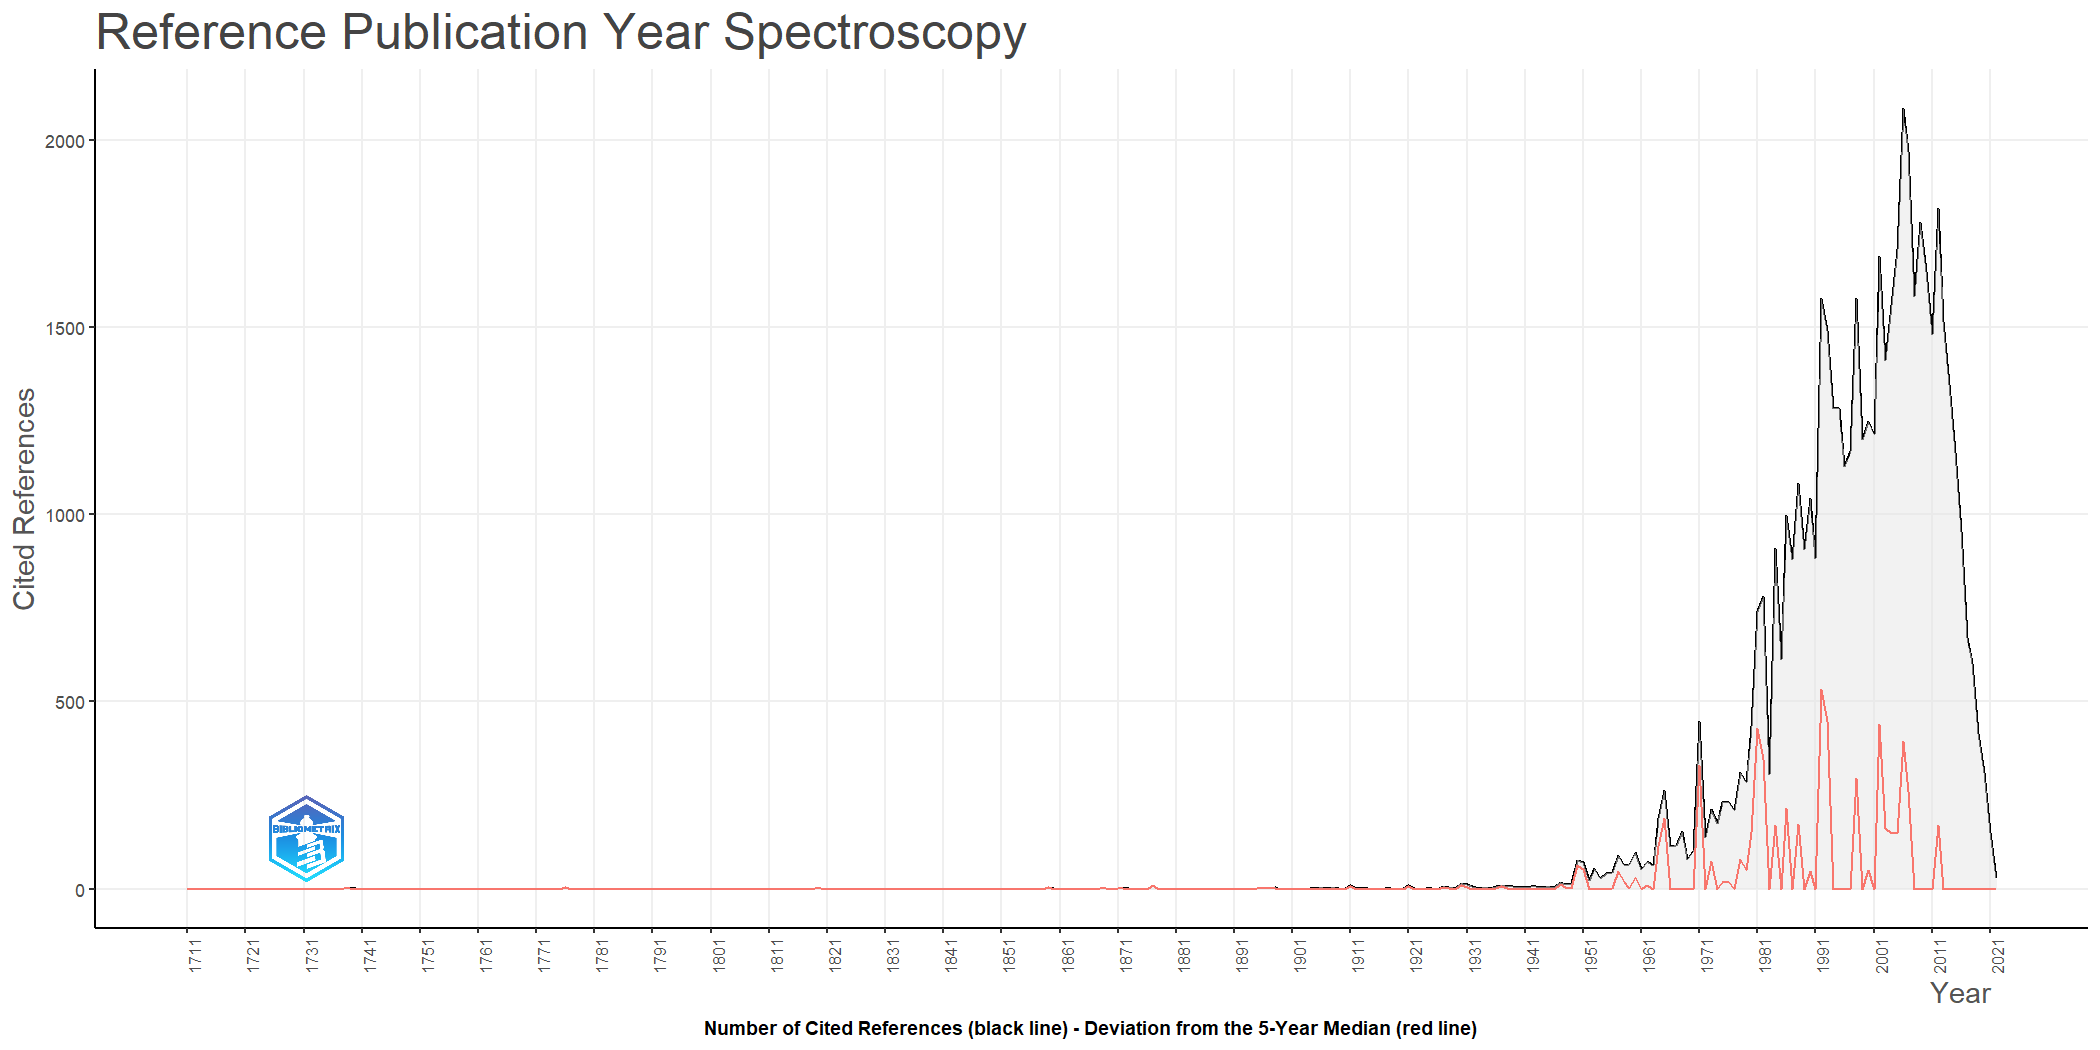
\includegraphics[width=1\textwidth]{exploratory-data-analysis/jvcalassio/PesqBibliogr/PrisonersDilemma/WoS-20221201/Dataset/ReferenceSpectroscopy-2022-12-03.png}
    \caption{Espectroscopia (RPYS) completa das referências do \dataset\ PD@jvcalassio.}
    \label{fig:PD@jvcalassio:ReferenceSpectroscopy}
\end{figure}

\subsection{Uso de palavras dentro dos artigos no \dataset}

As últimas das métricas aplicadas a documentos, disponíveis para aplicação no Bibliometrix é baseada na ocorrência de termos no texto dos documentos. A mais comum delas é baseada na simples contagem de frequência das palavras, como ilustra a figura \ref{fig:PD@jvcalassio:Word:Occurrences}, com os 40 termos mais frequentes em uso.

\begin{figure}
    \centering
    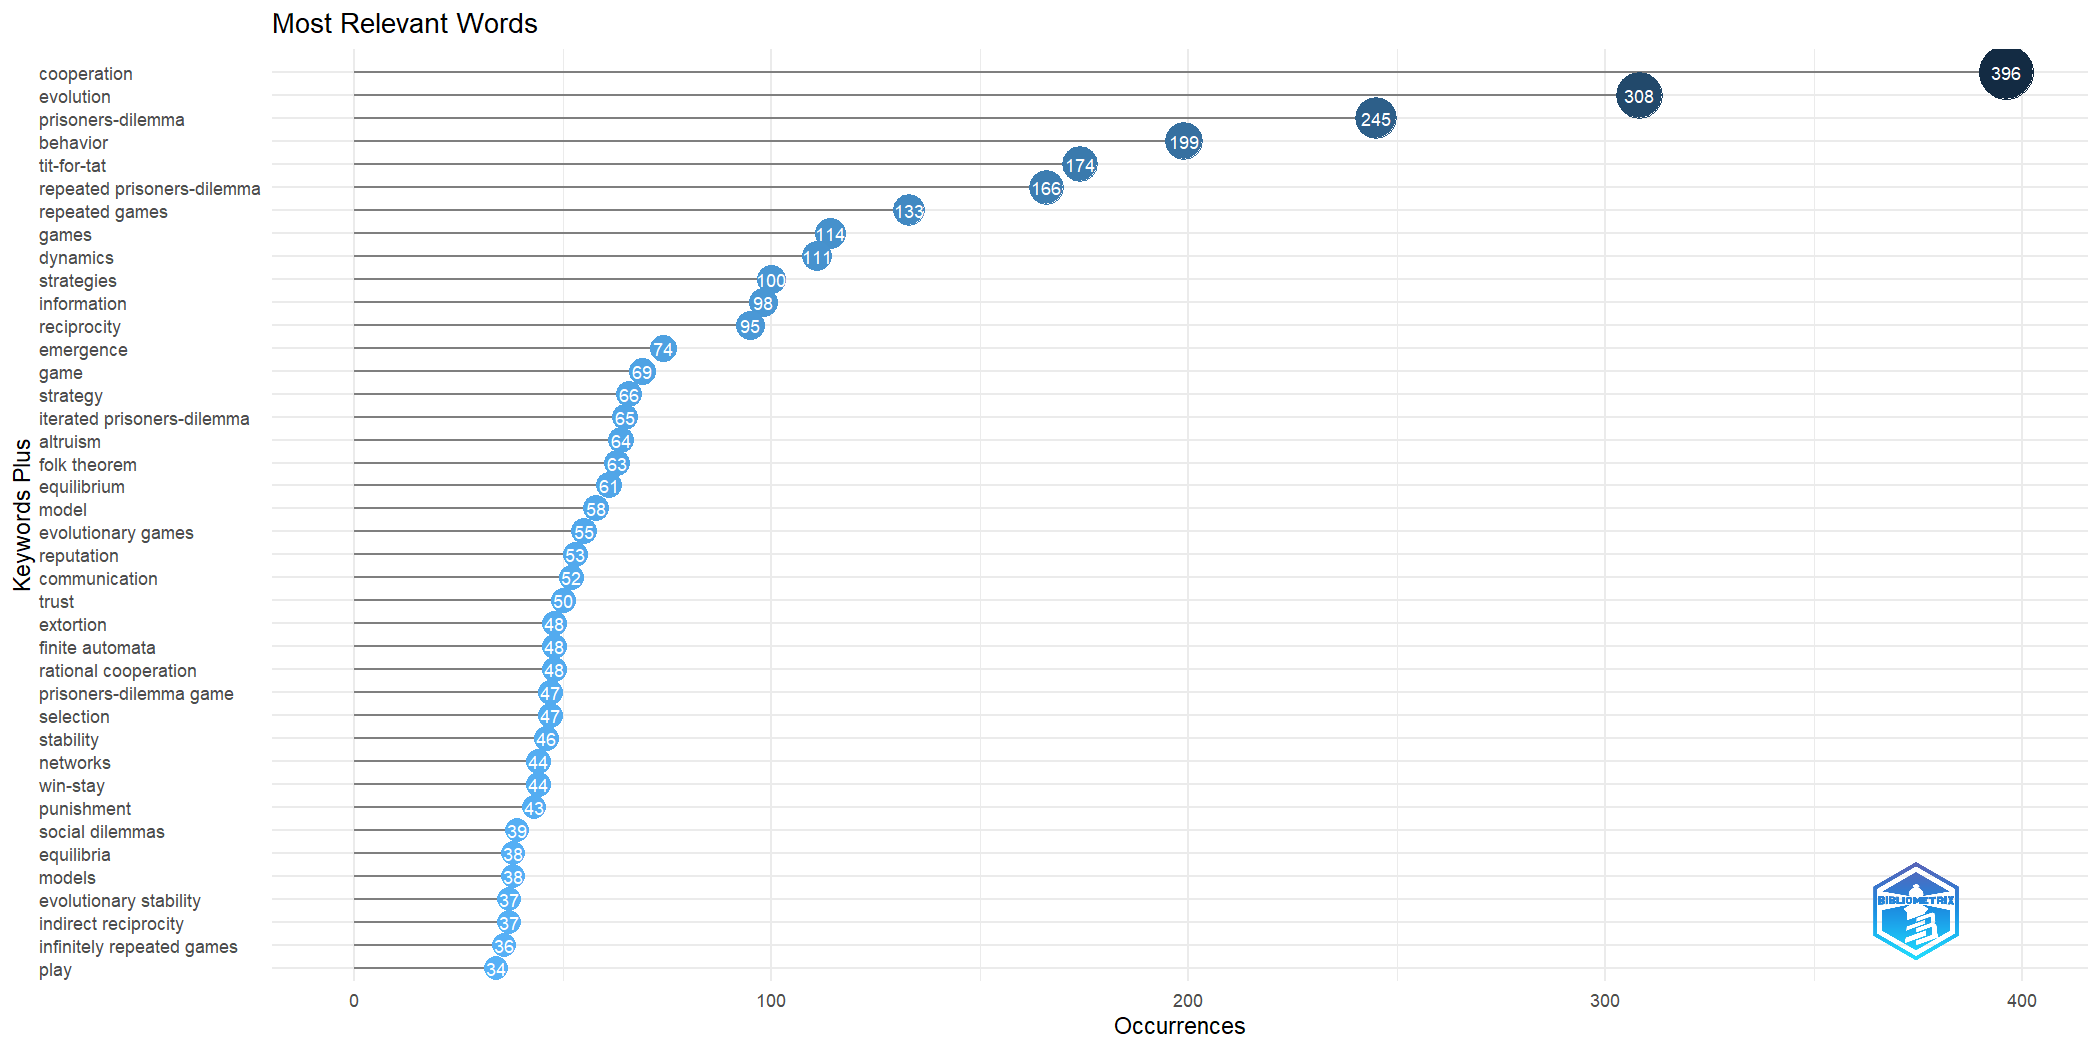
\includegraphics[width=1\textwidth]{exploratory-data-analysis/jvcalassio/PesqBibliogr/PrisonersDilemma/WoS-20221201/Dataset/MostRelevantWords-2022-12-03.png}
    \caption{40 palavras (termos) mais frequentes no \dataset\ PD@jvcalassio.}
    \label{fig:PD@jvcalassio:Word:Occurrences}
\end{figure}

Outras formas de apresentação alternativas são apresentadas nas duas figuras a seguir, que ilustram de forma diferente a mesma informação, como em:
\begin{description}
    \item [Word Cloud] Uma nuvem de palavras, na figura \ref{fig:PD@jvcalassio:WordCloud-100words}, com evidencias para as 100 palavras mais frequentes;
    \item [Tree Map] Um mapa em árvore, na figura \ref{fig:PD@jvcalassio:TreeMap}, com evidências para as 50 palavras mais frequentes;
\end{description}

\begin{figure}
    \centering
    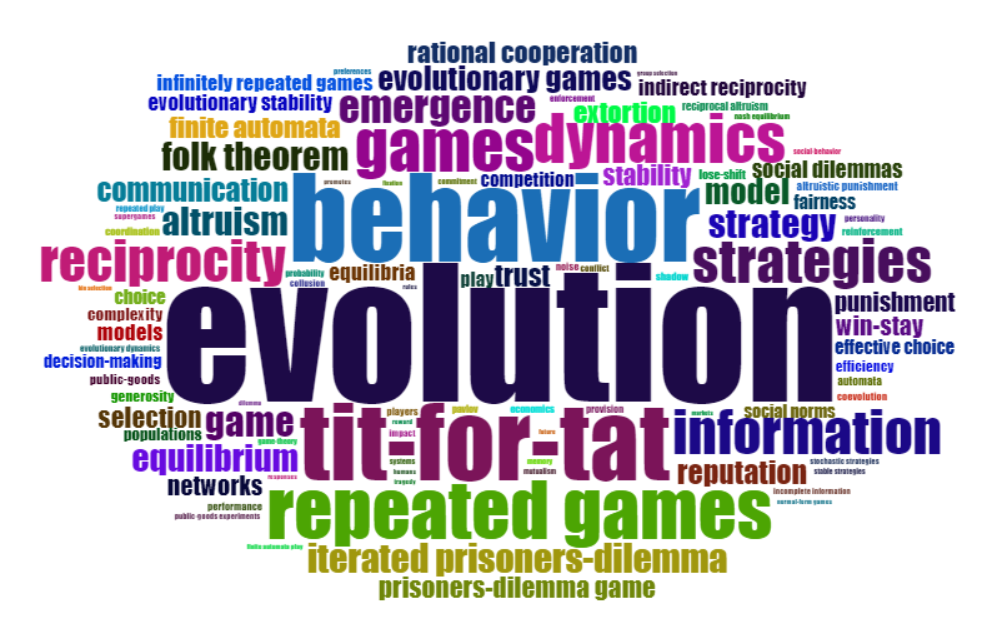
\includegraphics[width=1\textwidth]{exploratory-data-analysis/jvcalassio/PesqBibliogr/PrisonersDilemma/WoS-20221201/Dataset/WordCloud-100words.png}
    \caption{Nuvem dos 100 termos mais frequentes do \dataset\ PD@jvcalassio.}
    \label{fig:PD@jvcalassio:WordCloud-100words}
\end{figure}

\begin{figure}
    \centering
    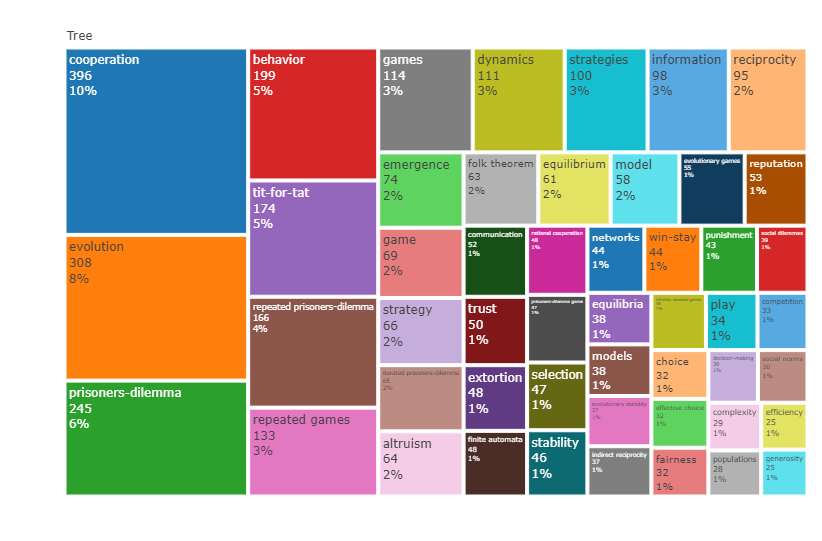
\includegraphics[width=1\textwidth]{exploratory-data-analysis/jvcalassio/PesqBibliogr/PrisonersDilemma/WoS-20221201/Dataset/TreeMap.png}
    \caption{\textit{Tree Map} dos 50 termos mais frequentes do \dataset\ PD@jvcalassio.}
    \label{fig:PD@jvcalassio:TreeMap}
\end{figure}

Por fim, o Bibliometrix permite apresentar o uso dos termos ordenado temporalmente, como nas duas figuras a seguir:

\begin{description}
    \item [Word Growth / Word Dynamics] que mostra o crescimento de uso das palavras mais frequentes, como na figura \ref{fig:PD@jvcalassio:WordDynamics};
    \item [Trending topics] que mostra as tendências para uso de determinadas palavras em determinadas faixas de tempo, como em \ref{fig:PD@jvcalassio:TrendTopics}. Para obtenção do gráfico foram determinados os seguintes valores para os parâmetros: frequência mínima de ocorrência para que um termo seja considerado = 15, quantidade máxima de tópicos por ano = 7.
\end{description}

\begin{figure}
    \centering
    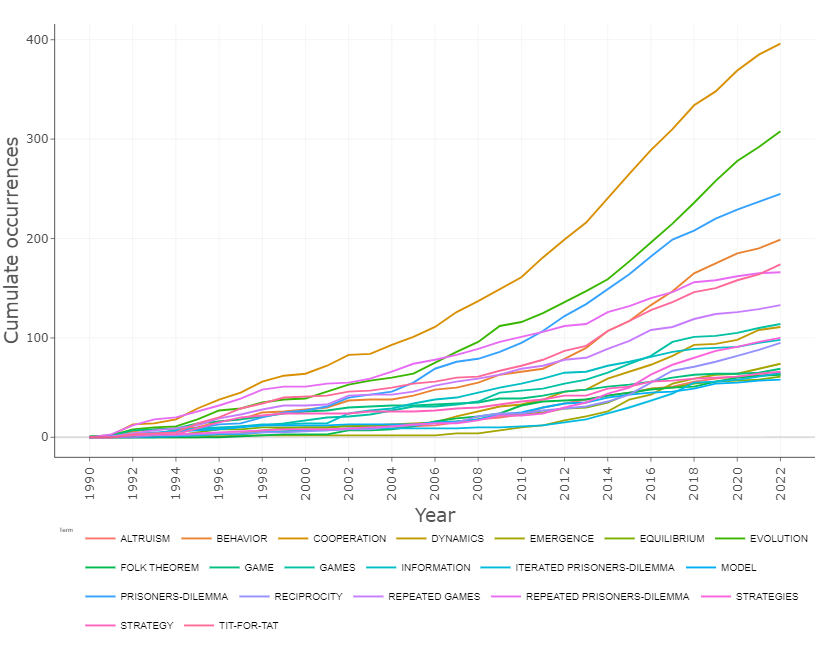
\includegraphics[width=1\textwidth]{exploratory-data-analysis/jvcalassio/PesqBibliogr/PrisonersDilemma/WoS-20221201/Dataset/WordDynamics-2022-12-03.png}
    \caption{Dinâmica de uso ao longo do tempo, dos 20 termos mais frequentes do \dataset\ PD@jvcalassio.}
    \label{fig:PD@jvcalassio:WordDynamics}
\end{figure}

\begin{figure}
    \centering
    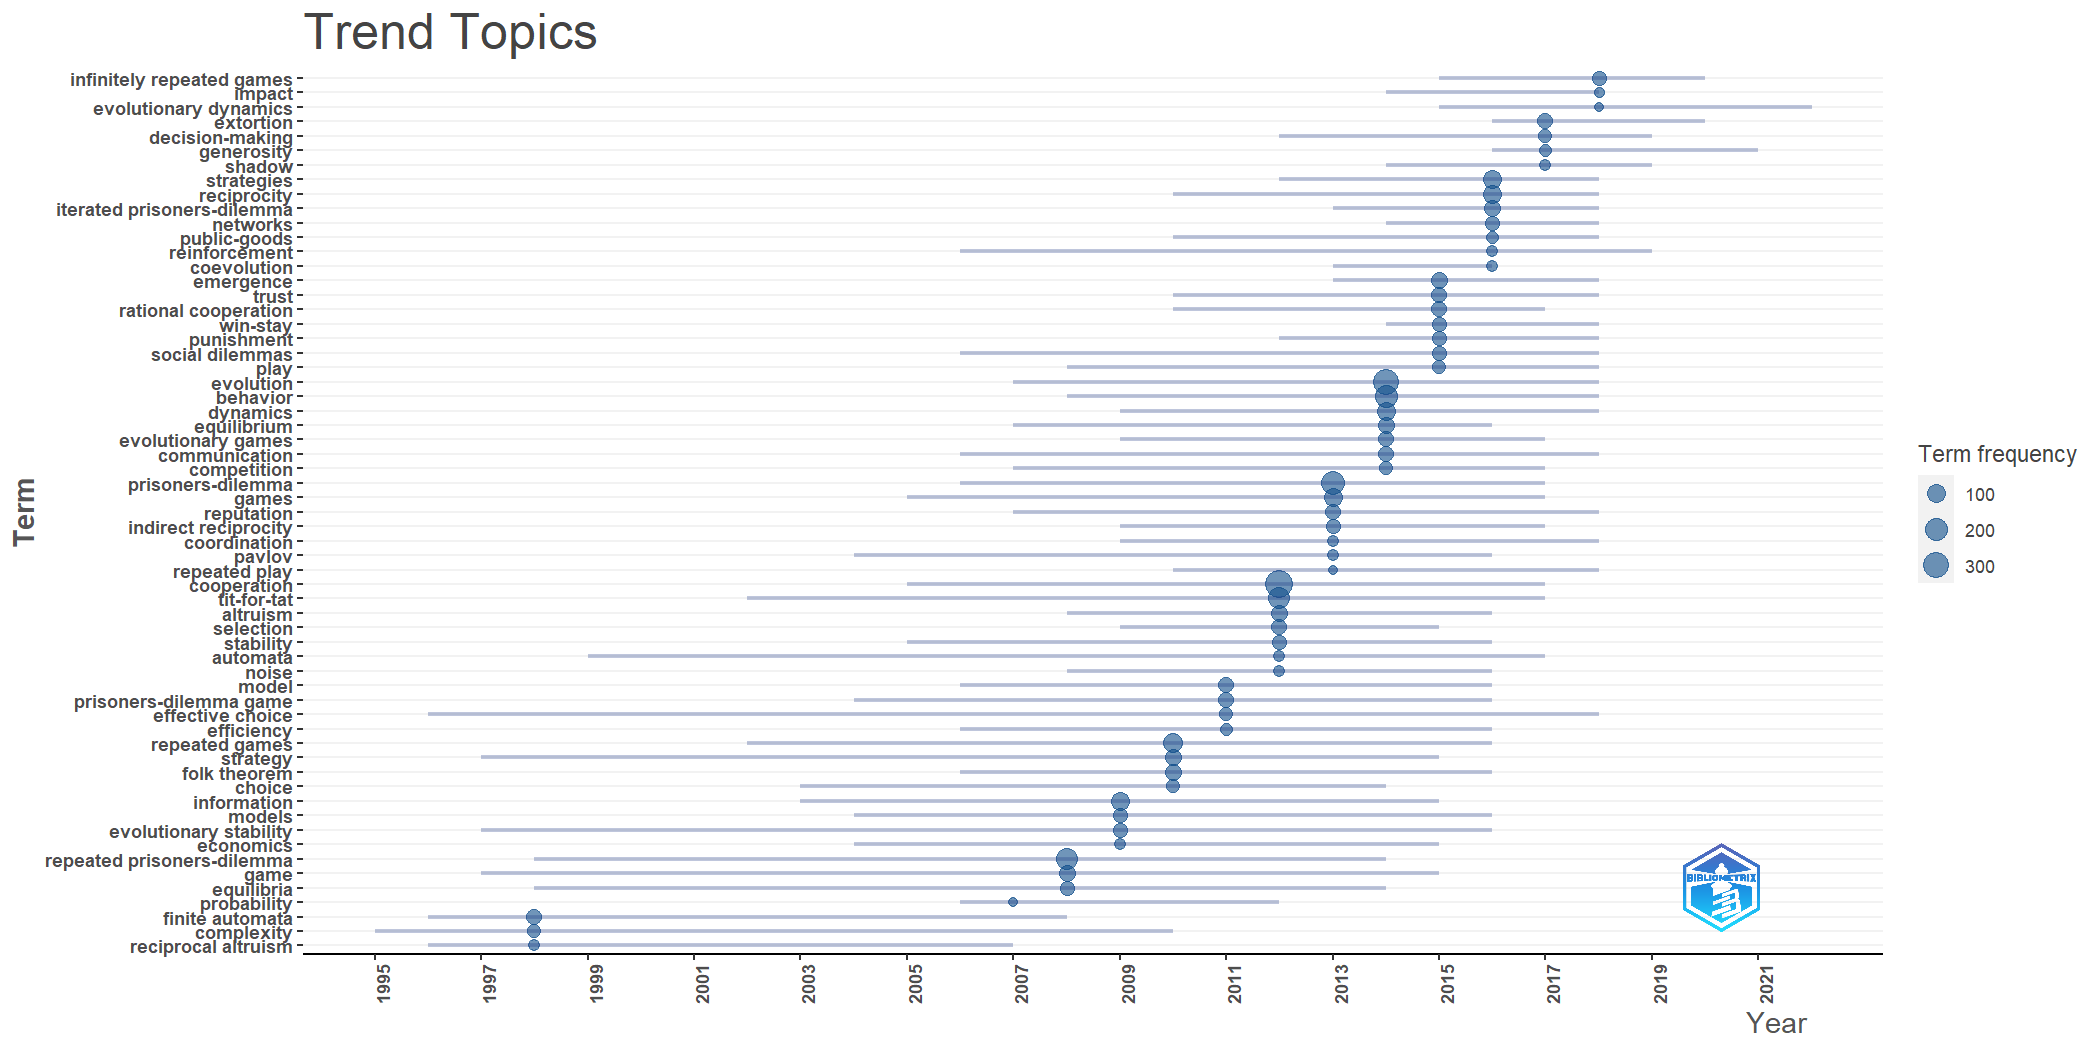
\includegraphics[width=1\textwidth]{exploratory-data-analysis/jvcalassio/PesqBibliogr/PrisonersDilemma/WoS-20221201/Dataset/TrendTopics-2022-12-03.png}
    \caption{\textit{Trending Topics} do \dataset\ PD@jvcalassio, WF = 15, WPY=7.}
    \label{fig:PD@jvcalassio:TrendTopics}
\end{figure}

\subsection{Autores mais produtivos no \dataset}

A figura \ref{fig:PD@jvcalassio:Author:Production} apresenta a lista ordenada e decrescente dos autores com maior número de artigos no \dataset.

\begin{figure}
    \centering
    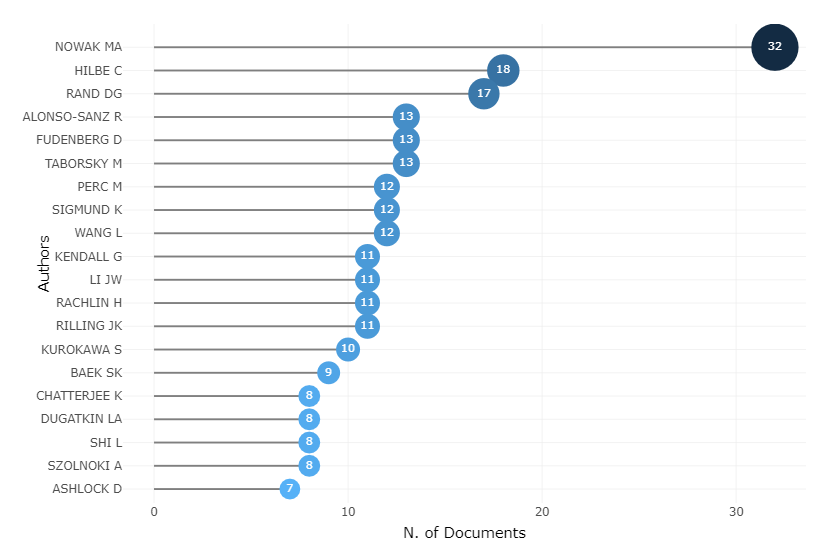
\includegraphics[width=1\textwidth]{exploratory-data-analysis/jvcalassio/PesqBibliogr/PrisonersDilemma/WoS-20221201/Dataset/MostRelevantAuthors-2022-12-03.png}
    \caption{20 autores com mais artigos no \dataset\ PD@jvcalassio.}
    \label{fig:PD@jvcalassio:Author:Production}
\end{figure}

\subsection{Autores mais relevantes localmente citados}

A figura \ref{fig:PD@jvcalassio:Author:LocalProduction} apresenta a lista ordenada e decrescente dos autores com maior número de artigos citados por outros artigos no \dataset. Esses são, possivelmente, os autores mais impactantes para o estado da arte no \dataset\ PD@jvcalassio.

\begin{figure}
    \centering
    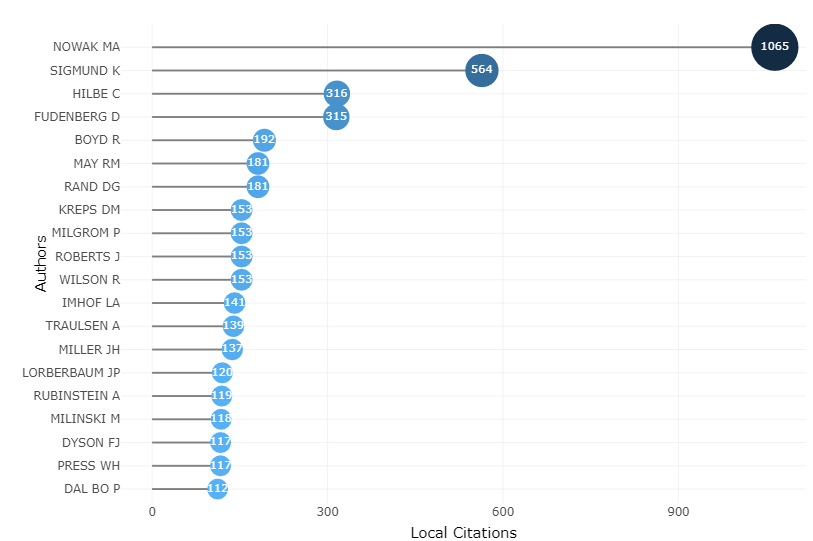
\includegraphics[width=1\textwidth]{exploratory-data-analysis/jvcalassio/PesqBibliogr/PrisonersDilemma/WoS-20221201/Dataset/MostRelevantAuthorsLocal-2022-12-03.png}
    \caption{20 autores com mais artigos no \dataset\ PD@jvcalassio.}
    \label{fig:PD@jvcalassio:Author:LocalProduction}
\end{figure}

\subsubsection{Variação da produtividade dos autores ao longo do tempo}

Os cientistas são seres humanos, que também tem um ciclo de vida de iniciante, muito produtivo, menos produtivo, e não produtivo.
Diagramas como o da figura \ref{fig:PD@jvcalassio:Author:TopAuthorsProductionOverTime} apresentam esse ciclo de vida, em relação ao \dataset\ PD@jvcalassio.

\begin{figure}
    \centering
    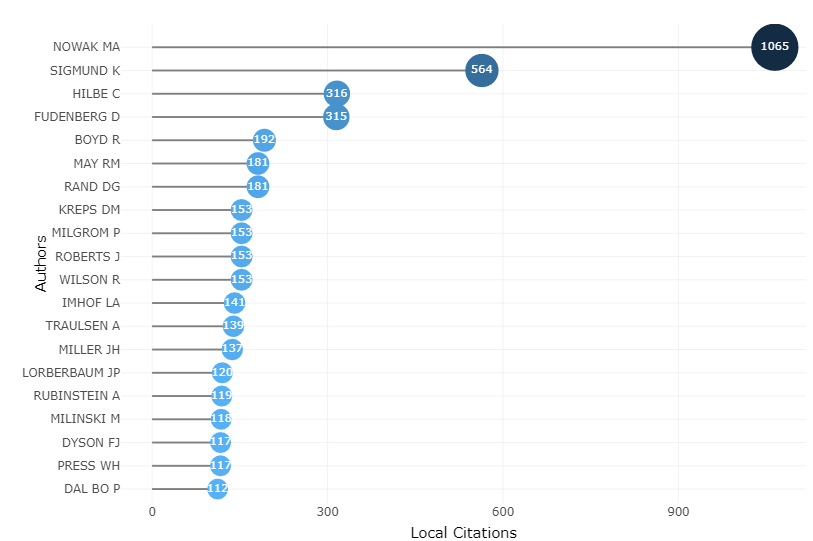
\includegraphics[width=1\textwidth]{exploratory-data-analysis/jvcalassio/PesqBibliogr/PrisonersDilemma/WoS-20221201/Dataset/MostRelevantAuthorsLocal-2022-12-03.png}
    \caption{Variação da produção dos autores de maior impacto, do \dataset\ PD@jvcalassio.}
    \label{fig:PD@jvcalassio:Author:TopAuthorsProductionOverTime}
\end{figure}

\subsection{Lei de Lotka}

A Lei de Lotka (ver \url{https://en.wikipedia.org/wiki/Lotka\%27s_law}) estabelece uma distribuição de frequência aproximadamente inversamente quadrática ou cúbica, para o número de artigos publicados pelos autores de qualquer área do conhecimento. Isso é, se 1000 pessoas publicam ao longo de sua contribuição para o campo de conhecimento apenas um documento, então
entre $1000/x^{2}$ a $1000/x^{3}$ publicam $x$ documentos. Ou seja, entre
$1000/2^{2}$ a $1000/2^{3}$ pessoas publicam dois documentos, $1000/3^{2}$ a $1000/3^{3}$ pessoas publicam três documentos etc.

Se os dados empíricos do \dataset\ são alinhados à essas curvas, então é correto supor que o \dataset\ é bem formado. Podemos verificar que há uma aproximação muito boa na figura \ref{fig:PD@jvcalassio:Author:Lotka}.

\begin{figure}
    \centering
    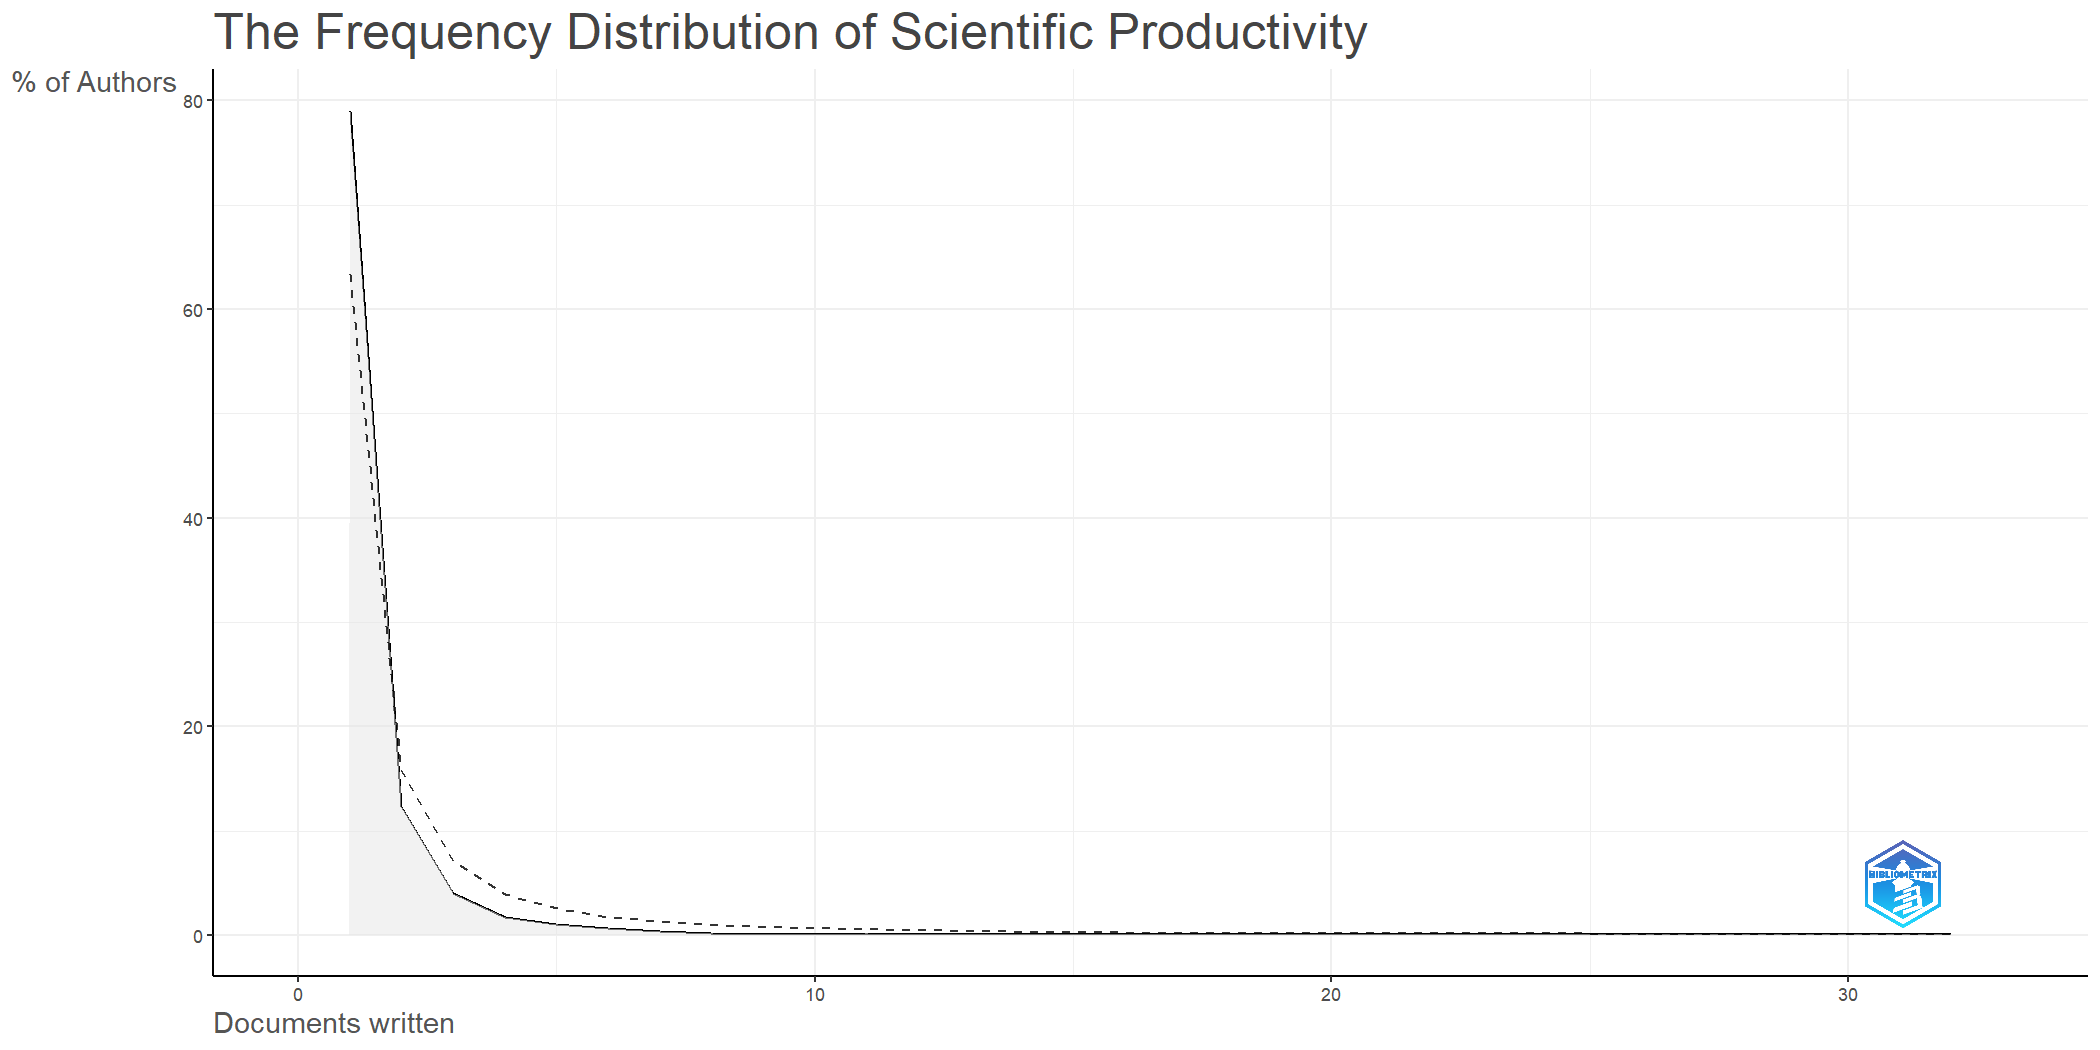
\includegraphics[width=1\textwidth]{exploratory-data-analysis/jvcalassio/PesqBibliogr/PrisonersDilemma/WoS-20221201/Dataset/LotkaLaw-2022-12-03.png}
    \caption{Comparação do \dataset\ PD@jvcalassio com a formulação geral da Lei de Lotka.}
    \label{fig:PD@jvcalassio:Author:Lotka}
\end{figure}

\subsection{Medidas de Impacto dos Autores}

A partir da medida básica de citações (TC) podem ser criados vários índices, sendo os mais conhecidos os índices H (Ver \url{https://en.wikipedia.org/wiki/H-index}), G (Ver \url{https://en.wikipedia.org/wiki/G-index})e M (ver \url{https://en.wikipedia.org/wiki/Author-level_metrics#m-index}).

As tabelas \ref{tab:PD@jvcalassio:Author:ImpactoH}, \ref{tab:PD@jvcalassio:Author:ImpactoG}, \ref{tab:PD@jvcalassio:Author:ImpactoM} e \ref{tab:PD@jvcalassio:Author:ImpactoQtdPublicacoes} mostram os autores mais proeminentes do \dataset\ ordenados com base em um desses índices ou com o simples volume total de publicação, em comparação aos demais índices.

Além dos índices e da quantidade total de citações (coluna TC), apresenta-se o volume de publicações (NP) e o ano de primeira publicação do autor (PY Start).

Observe que os índices H e G tendem a valorizar os autores mais estabilizados, enquanto que o índice M mostra os autores mais recentes, que tem menos anos de publicação.

Observe, adicionalmente, que a base para cálculo desses índices é o número total de citações, que tem alcance global, enquanto que o número de artigos publicados é o valor local.

\begin{table}[htp]
    \centering
    \footnotesize
    % \csvreader[
    % separator=semicolon,
    % tabular = {|r|l|r|r|r|r|r|r|},
    % filter={\value{csvrow}<40},
    % %,filter not strcmp={\csvcolii}{},
    % table head = \hline\hline \# & Autor & Índice H & Índice G & Índice M & TC & NP & PY Start\\ \hline\hline,
    % table foot = \hline\hline]
    % {exploratory-data-analysis/jvcalassio/PesqBibliogr/PrisonersDilemma/WoS-20221201/Dataset/Author-Impact-H.csv}
    % {}
    % { \thecsvrow & \csvcoli & \csvcolii & \csvcoliii & \csvcoliv & \csvcolv & \csvcolvi & \csvcolvii}
    \begin{tabular}{|l|l|l|l|l|l|l|}
    \hline
        Element & h\_index & g\_index & m\_index & TC & NP & PY\_start \\ \hline
        NOWAK MA & 23 & 32 & 0.742 & 7741 & 32 & 1992 \\ \hline
        HILBE C & 15 & 18 & 1.071 & 869 & 18 & 2009 \\ \hline
        RAND DG & 15 & 17 & 1.071 & 1142 & 17 & 2009 \\ \hline
        SIGMUND K & 12 & 12 & 0.364 & 3198 & 12 & 1990 \\ \hline
        FUDENBERG D & 11 & 13 & 0.579 & 1564 & 13 & 2004 \\ \hline
        RILLING JK & 11 & 11 & 0.524 & 1892 & 11 & 2002 \\ \hline
        PERC M & 10 & 12 & 0.625 & 819 & 12 & 2007 \\ \hline
        RACHLIN H & 9 & 11 & 0.375 & 354 & 11 & 1999 \\ \hline
        TABORSKY M & 9 & 13 & 0.500 & 372 & 13 & 2005 \\ \hline
        DUGATKIN LA & 8 & 8 & 0.250 & 512 & 8 & 1991 \\ \hline
    \end{tabular}
    \caption{10 autores de maior impacto no \dataset\ PD@jvcalassio, conforme o índice H.}
    \label{tab:PD@jvcalassio:Author:ImpactoH}
\end{table}

\begin{table}[htp]
    \centering
    \footnotesize
    % \csvreader[
    % separator=semicolon,
    % tabular = {|r|l|r|r|r|r|r|r|},
    % filter={\value{csvrow}<40},
    % %,filter not strcmp={\csvcolii}{},
    % table head = \hline\hline \# & Autor & Índice H & Índice G & Índice M & TC & NP & PY Start\\ \hline\hline,
    % table foot = \hline\hline]
    % {exploratory-data-analysis/jvcalassio/PesqBibliogr/PrisonersDilemma/WoS-20221201/Dataset/Author-Impact-G.csv}
    % {}
    % { \thecsvrow & \csvcoli & \csvcolii & \csvcoliii & \csvcoliv & \csvcolv & \csvcolvi & \csvcolvii}
    \begin{tabular}{|l|l|l|l|l|l|l|}
    \hline
        Element & h\_index & g\_index & m\_index & TC & NP & PY\_start \\ \hline
        NOWAK MA & 23 & 32 & 0.742 & 7741 & 32 & 1992 \\ \hline
        HILBE C & 15 & 18 & 1.071 & 869 & 18 & 2009 \\ \hline
        RAND DG & 15 & 17 & 1.071 & 1142 & 17 & 2009 \\ \hline
        FUDENBERG D & 11 & 13 & 0.579 & 1564 & 13 & 2004 \\ \hline
        TABORSKY M & 9 & 13 & 0.500 & 372 & 13 & 2005 \\ \hline
        ALONSO-SANZ R & 7 & 13 & 0.350 & 178 & 13 & 2003 \\ \hline
        SIGMUND K & 12 & 12 & 0.364 & 3198 & 12 & 1990 \\ \hline
        PERC M & 10 & 12 & 0.625 & 819 & 12 & 2007 \\ \hline
        WANG L & 6 & 12 & 0.500 & 193 & 12 & 2011 \\ \hline
        RILLING JK & 11 & 11 & 0.524 & 1892 & 11 & 2002 \\ \hline
    \end{tabular}
    \caption{10 autores de maior impacto no \dataset\ PD@jvcalassio, conforme o índice G.}
    \label{tab:PD@jvcalassio:Author:ImpactoG}
\end{table}

\begin{table}[htp]
    \centering
    \footnotesize
    % \csvreader[
    % separator=semicolon,
    % tabular = {|r|l|r|r|r|r|r|r|},
    % filter={\value{csvrow}<40},
    % %,filter not strcmp={\csvcolii}{},
    % table head = \hline\hline \# & Autor & Índice H & Índice G & Índice M & TC & NP & PY Start\\ \hline\hline,
    % table foot = \hline\hline]
    % {exploratory-data-analysis/jvcalassio/PesqBibliogr/PrisonersDilemma/WoS-20221201/Dataset/Author-Impact-M.csv}
    % {}
    % { \thecsvrow & \csvcoli & \csvcolii & \csvcoliii & \csvcoliv & \csvcolv & \csvcolvi & \csvcolvii}
    \begin{tabular}{|l|l|l|l|l|l|l|}
    \hline
        Element & h\_index & g\_index & m\_index & TC & NP & PY\_start \\ \hline
        HILBE C & 15 & 18 & 1.071 & 869 & 18 & 2009 \\ \hline
        RAND DG & 15 & 17 & 1.071 & 1142 & 17 & 2009 \\ \hline
        TERADA K & 3 & 3 & 1.000 & 22 & 3 & 2020 \\ \hline
        UEDA M & 2 & 2 & 1.000 & 10 & 2 & 2021 \\ \hline
        AL-GHARAIBEH RS & 1 & 1 & 1.000 & 4 & 1 & 2022 \\ \hline
        ALI MZ & 1 & 1 & 1.000 & 4 & 1 & 2022 \\ \hline
        AYAD R & 1 & 1 & 1.000 & 1 & 1 & 2022 \\ \hline
        CHAKRABORTY S & 1 & 1 & 1.000 & 1 & 1 & 2022 \\ \hline
        DE DREU CKW & 1 & 1 & 1.000 & 1 & 1 & 2022 \\ \hline
        DENG WN & 1 & 1 & 1.000 & 1 & 1 & 2022 \\ \hline
    \end{tabular}
    \caption{10 autores de maior impacto no \dataset\ PD@jvcalassio, conforme o índice M.}
    \label{tab:PD@jvcalassio:Author:ImpactoM}
\end{table}

\begin{table}[htp]
    \centering
    \footnotesize
    % \csvreader[
    % separator=semicolon,
    % tabular = {|r|l|r|r|r|r|r|r|},
    % filter={\value{csvrow}<40},
    % %,filter not strcmp={\csvcolii}{},
    % table head = \hline\hline \# & Autor & Índice H & Índice G & Índice M & TC & NP & PY Start\\ \hline\hline,
    % table foot = \hline\hline]
    % {exploratory-data-analysis/jvcalassio/PesqBibliogr/PrisonersDilemma/WoS-20221201/Dataset/Author-Impact-TC.csv}
    % {}
    % { \thecsvrow & \csvcoli & \csvcolii & \csvcoliii & \csvcoliv & \csvcolv & \csvcolvi & \csvcolvii}
    \begin{tabular}{|l|l|l|l|l|l|l|}
    \hline
        Element & h\_index & g\_index & m\_index & TC & NP & PY\_start \\ \hline
        NOWAK MA & 23 & 32 & 0.742 & 7741 & 32 & 1992 \\ \hline
        SIGMUND K & 12 & 12 & 0.364 & 3198 & 12 & 1990 \\ \hline
        MAY RM & 2 & 2 & 0.065 & 2984 & 2 & 1992 \\ \hline
        RILLING JK & 11 & 11 & 0.524 & 1892 & 11 & 2002 \\ \hline
        PAGNONI G & 6 & 6 & 0.286 & 1602 & 6 & 2002 \\ \hline
        FUDENBERG D & 11 & 13 & 0.579 & 1564 & 13 & 2004 \\ \hline
        RAND DG & 15 & 17 & 1.071 & 1142 & 17 & 2009 \\ \hline
        KREPS DM & 1 & 1 & 0.024 & 1115 & 1 & 1982 \\ \hline
        MILGROM P & 1 & 1 & 0.024 & 1115 & 1 & 1982 \\ \hline
        ROBERTS J & 1 & 1 & 0.024 & 1115 & 1 & 1982 \\ \hline
    \end{tabular}
    \caption{10 autores de maior impacto no \dataset\ PD@jvcalassio, conforme a quantidade de vezes que seus artigos foram globalmente citados.}
    \label{tab:PD@jvcalassio:Author:ImpactoQtdPublicacoes}
\end{table}

\subsection{Filiações dos autores às instituições de P\&D}

Os autores de documentos científicos são filiados como estudantes ou empregados em universidades e centros de pesquisa, e quando os publicam colocam o nome de suas filiações, criando a possibilidade de produção de \textit{rankings} para essas instituições. A figura \ref{fig:PD@jvcalassio:Most-Relevant-Affiliations} apresenta as 20 instituições com maior produtividade, conforme o volume de artigos publicados presentes no \dataset. Ou seja, é nas instituições listadas na tabela onde possivelmente está mais avançado o conhecimento nesse tema. 

\begin{figure}
    \centering
    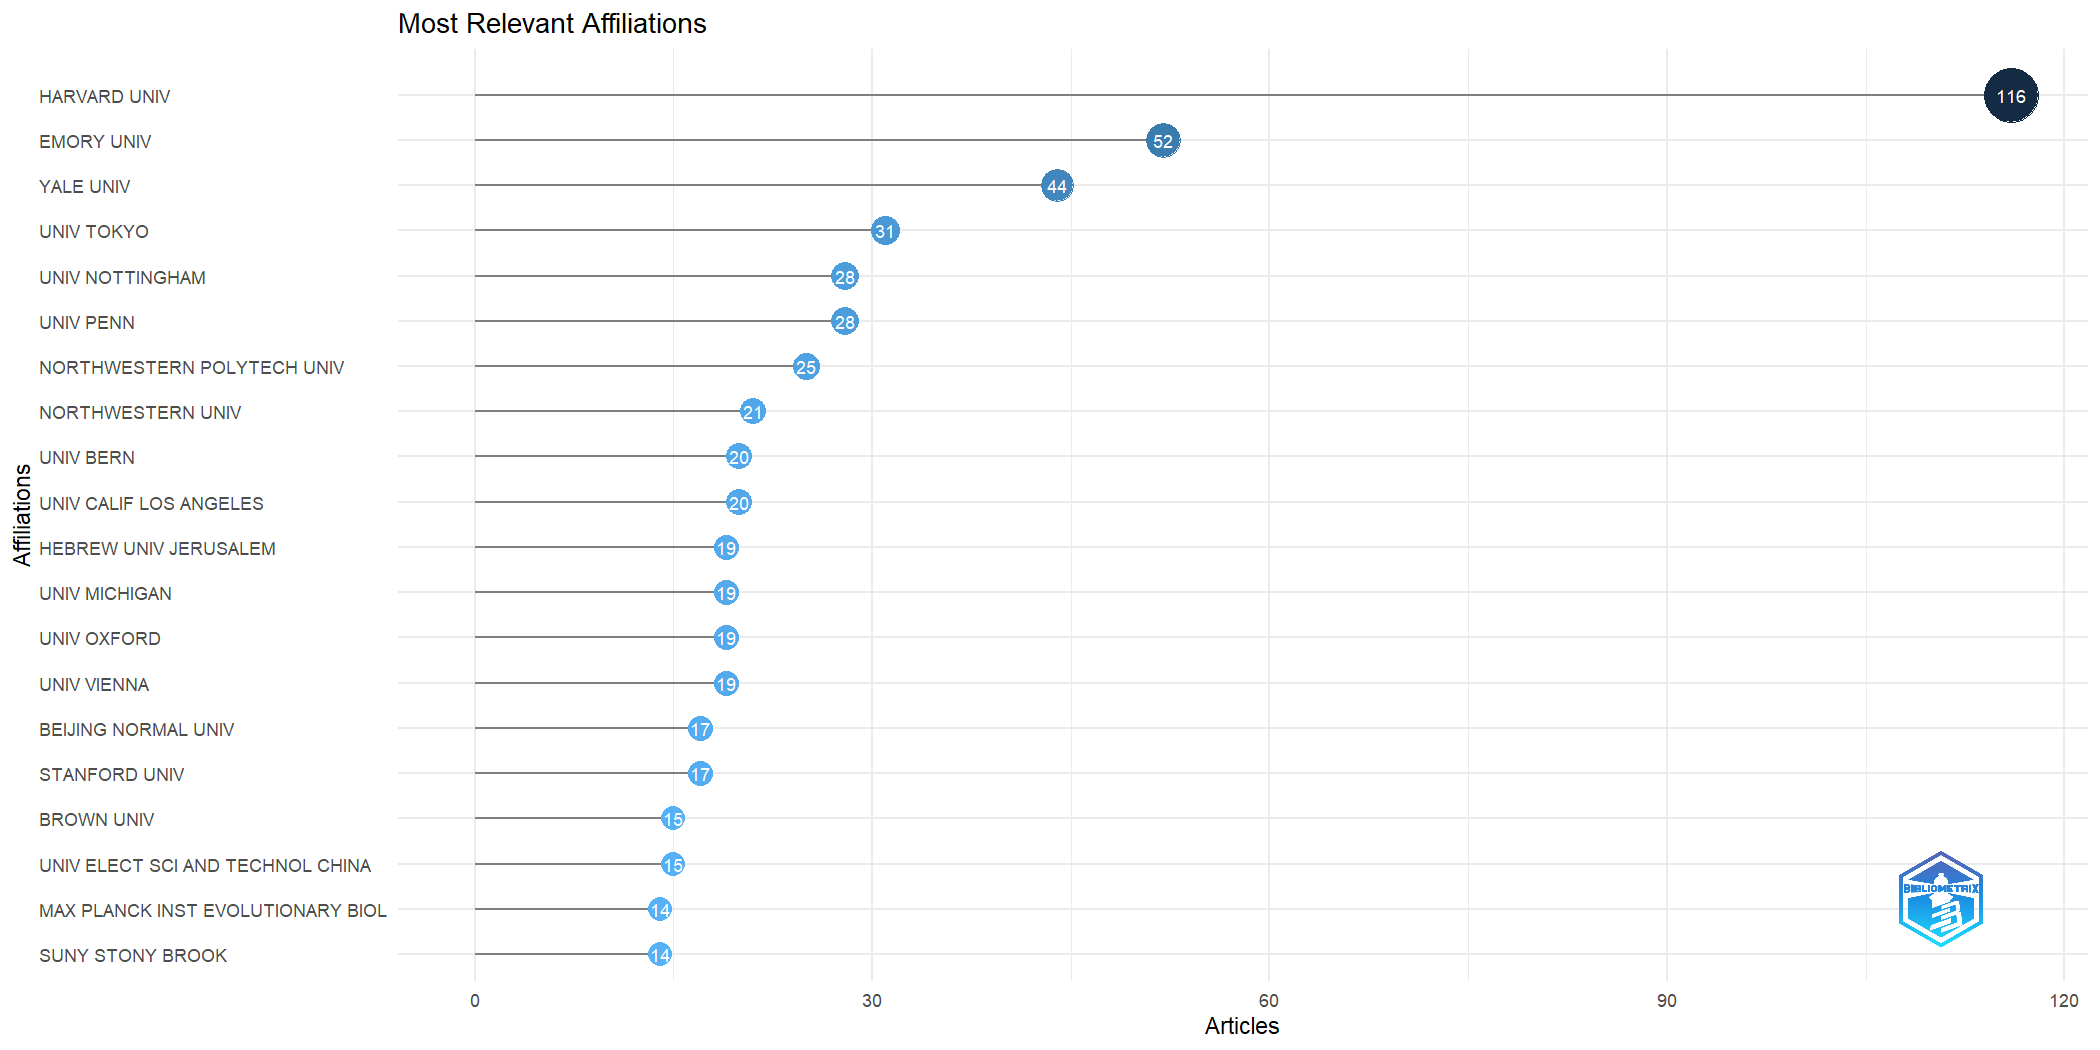
\includegraphics[width=1\textwidth]{exploratory-data-analysis/jvcalassio/PesqBibliogr/PrisonersDilemma/WoS-20221201/Dataset/MostRelevantAffiliations-2022-12-03.png}
    \caption{40 Instituições mais produtivas no tema do \dataset\ PD@jvcalassio, conforme a quantidade de artigos publicados por pessoas a elas filiadas.}
    \label{fig:PD@jvcalassio:Most-Relevant-Affiliations}
\end{figure}

\subsection{Filiações dos autores aos Países}

As instituições às quais são filiados os autores são sediadas em países, o que permite estimar a produtividade e (ou) impacto dos países em um tema de conhecimento específico, como ilustra a tabela \ref{tab:PD@jvcalassio:Most-Cited-Countries}, que mostra a quantidade de citações obtidas pelos artigos das instituições sediadas nesses países.

\begin{table}[htp]
    \centering
    \footnotesize
    % \csvreader[
    % separator=semicolon,
    % tabular = {|r|l|r|r|},
    % filter={\value{csvrow}<40},
    % %,filter not strcmp={\csvcolii}{},
    % table head = \hline\hline \# & País de Filiação & Qtd. Citações & Média de Citação por Artigo\\ \hline\hline,
    % table foot = \hline\hline]
    % {exploratory-data-analysis/jvcalassio/PesqBibliogr/PrisonersDilemma/WoS-20221201/Dataset/Most-Cited-Countries.csv}
    % {}
    % { \thecsvrow & \csvcoli & \csvcolii & \csvcoliii}
    \begin{tabular}{|l|l|l|}
    \hline
        Country & TC & Average Article Citations \\ \hline
        USA & 20233 & 42.96 \\ \hline
        UNITED KINGDOM & 8313 & 70.45 \\ \hline
        GERMANY & 2197 & 30.94 \\ \hline
        CHINA & 1708 & 12.94 \\ \hline
        SWITZERLAND & 1497 & 45.36 \\ \hline
        JAPAN & 1369 & 16.49 \\ \hline
        ISRAEL & 1186 & 37.06 \\ \hline
        NETHERLANDS & 1158 & 39.93 \\ \hline
        CANADA & 1026 & 17.10 \\ \hline
        AUSTRIA & 999 & 49.95 \\ \hline
        HUNGARY & 834 & 83.40 \\ \hline
        SPAIN & 665 & 16.63 \\ \hline
        FRANCE & 491 & 15.34 \\ \hline
        AUSTRALIA & 369 & 15.38 \\ \hline
        SINGAPORE & 359 & 59.83 \\ \hline
        ITALY & 294 & 15.47 \\ \hline
        KOREA & 229 & 9.54 \\ \hline
        BRAZIL & 220 & 27.50 \\ \hline
        PORTUGAL & 194 & 24.25 \\ \hline
        BELGIUM & 186 & 20.67 \\ \hline
        SWEDEN & 186 & 15.50 \\ \hline
        SLOVENIA & 153 & 51.00 \\ \hline
        INDIA & 135 & 16.88 \\ \hline
        FINLAND & 121 & 17.29 \\ \hline
        LUXEMBOURG & 97 & 48.50 \\ \hline
    \end{tabular}
    \caption{25 países com maior impacto de citações no tema do \dataset\ PD@jvcalassio.}
    \label{tab:PD@jvcalassio:Most-Cited-Countries}
\end{table}

\subsection{Países dos autores principais dos artigos}

Cada artigo escrito por mais de um autor tem um autor responsável por receber as correspondências relativas ao artigo. Esse é o  \textit{wordthor}. A figura \ref{fig:PD@jvcalassio:Corresponding-Authors-Country} apresenta, em ordem do maior para o menor volume de correspondentes por artigo, o volume publicado por cada país. SCP são as publicações cujos autores são todos do mesmo país. MCP envolve autores de mais de um país.

\begin{figure}
    \centering
    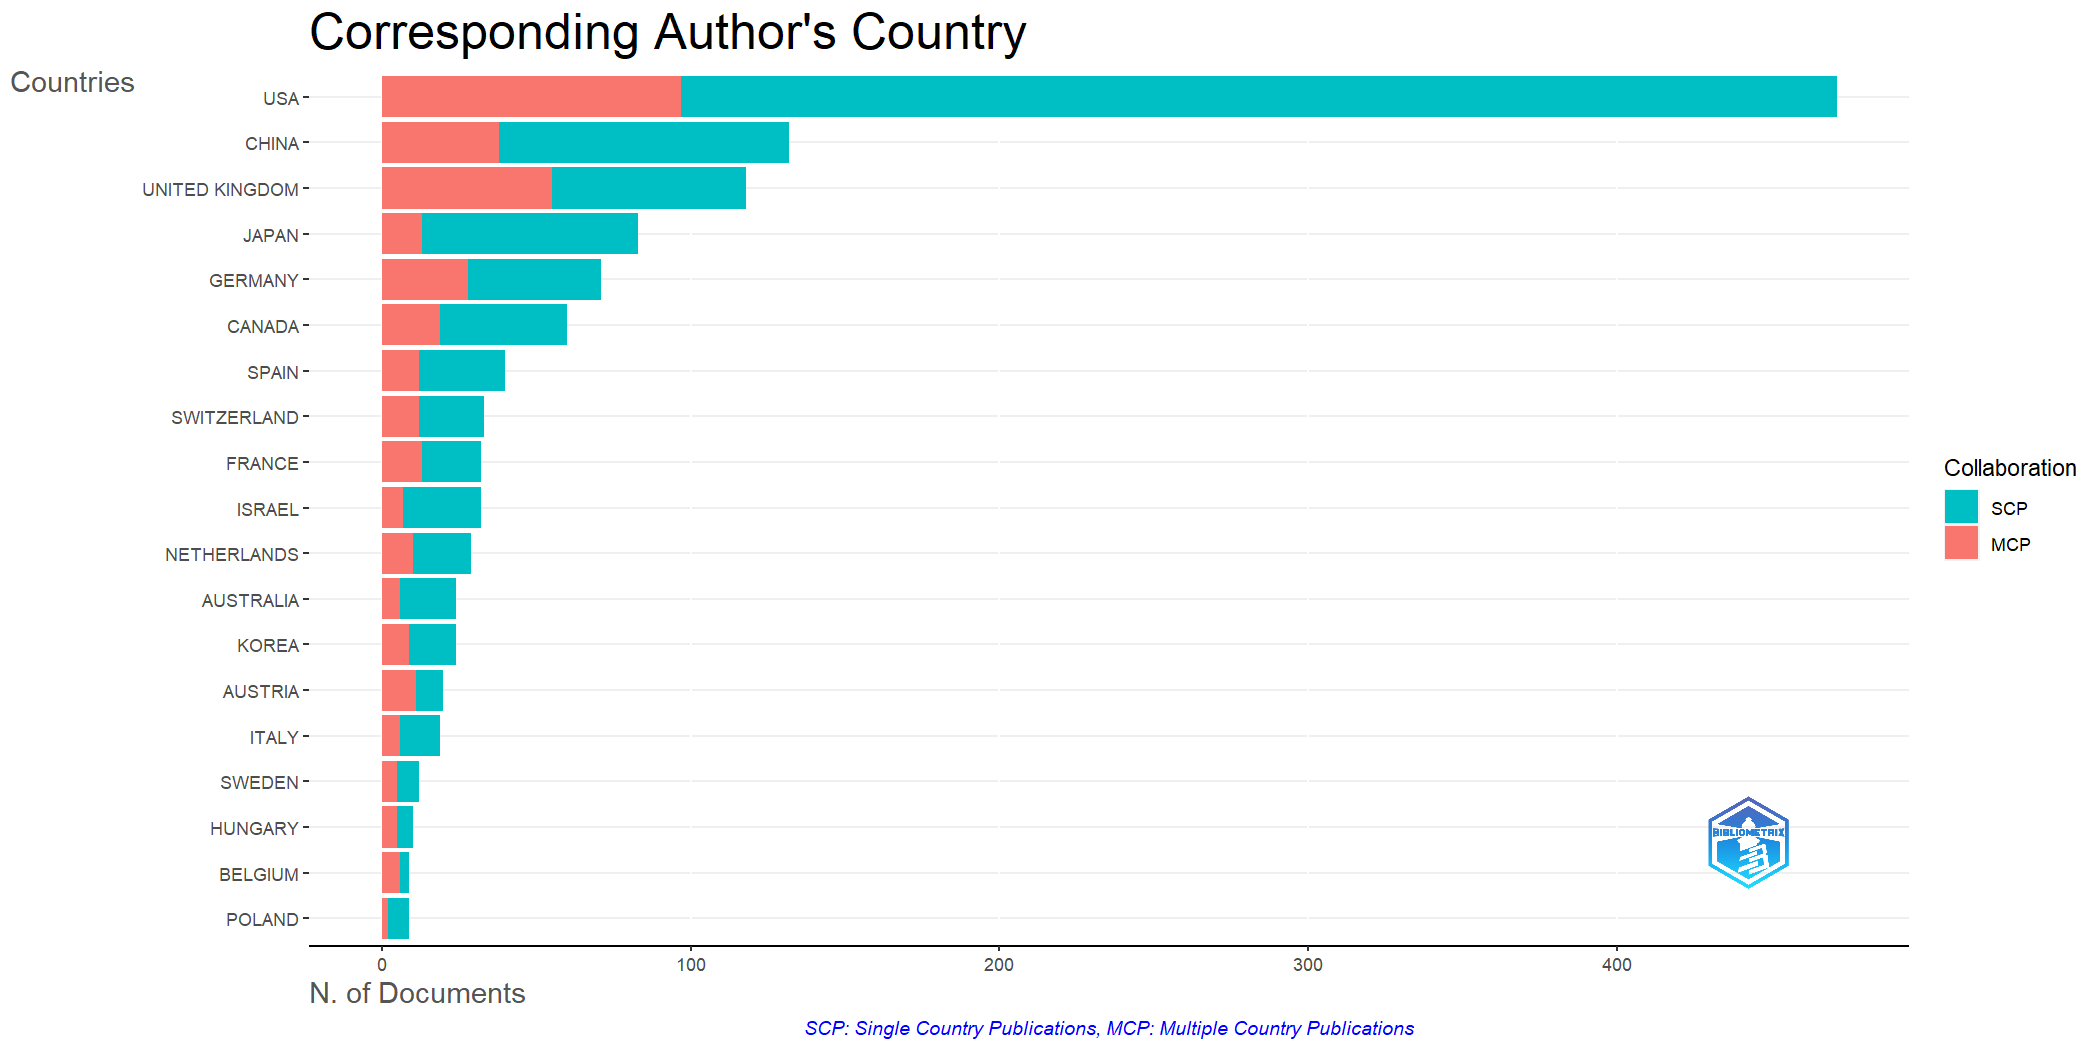
\includegraphics[width=1\textwidth]{exploratory-data-analysis/jvcalassio/PesqBibliogr/PrisonersDilemma/WoS-20221201/Dataset/MostRelevantCountries-2022-12-03.png}
    \caption{Variação da produção dos autores de maior impacto, do \dataset\ PD@jvcalassio.}
    \label{fig:PD@jvcalassio:Corresponding-Authors-Country}
\end{figure}

\subsection{Fontes mais relevantes, conforme número de artigos publicados sobre o tema}

Conforme podemos visualizar na figura \ref{fig:PD@jvcalassio:Most-Relevant-Sources}, a fonte mais relevante nesse tema é o \textit{Journal of Theoretical Biology}, se utilizarmos como critério o número de artigos publicados.

\begin{figure}
    \centering
    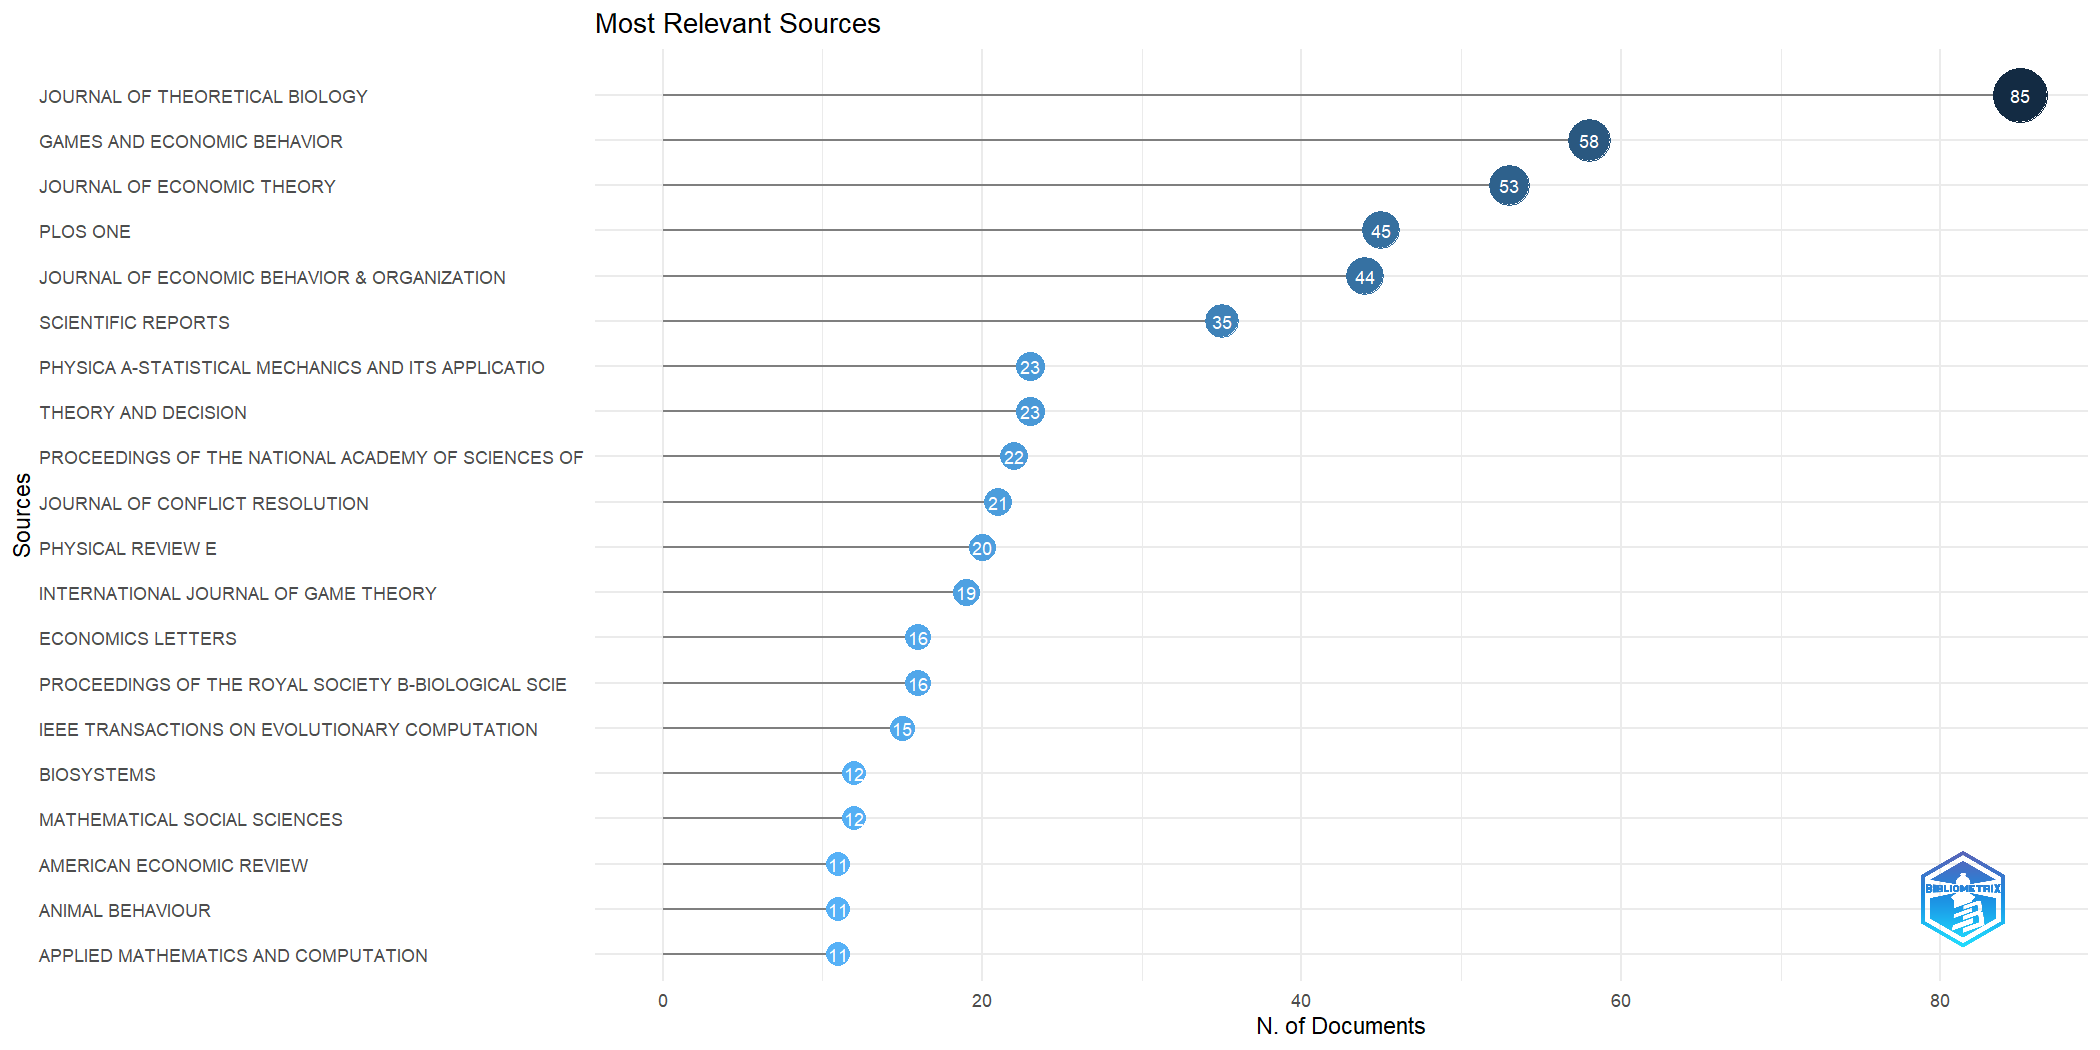
\includegraphics[width=1\textwidth]{exploratory-data-analysis/jvcalassio/PesqBibliogr/PrisonersDilemma/WoS-20221201/Dataset/MostRelevantSources-2022-12-03.png}
    \caption{Revistas mais relevantes no  \dataset\ PD@jvcalassio.}
    \label{fig:PD@jvcalassio:Most-Relevant-Sources}
\end{figure}

\subsection{Fontes mais relevantes, conforme o número de citações na lista de referências locais}

Conforme podemos visualizar na figura \ref{fig:PD@jvcalassio:Most-Local-Cited-Sources(from-Reference-Lists).png}, a fonte mais relevante nesse tema é a \textit{Nature}, se utilizarmos como critério o número de citações na lista de referências locais.

\begin{figure}
    \centering
    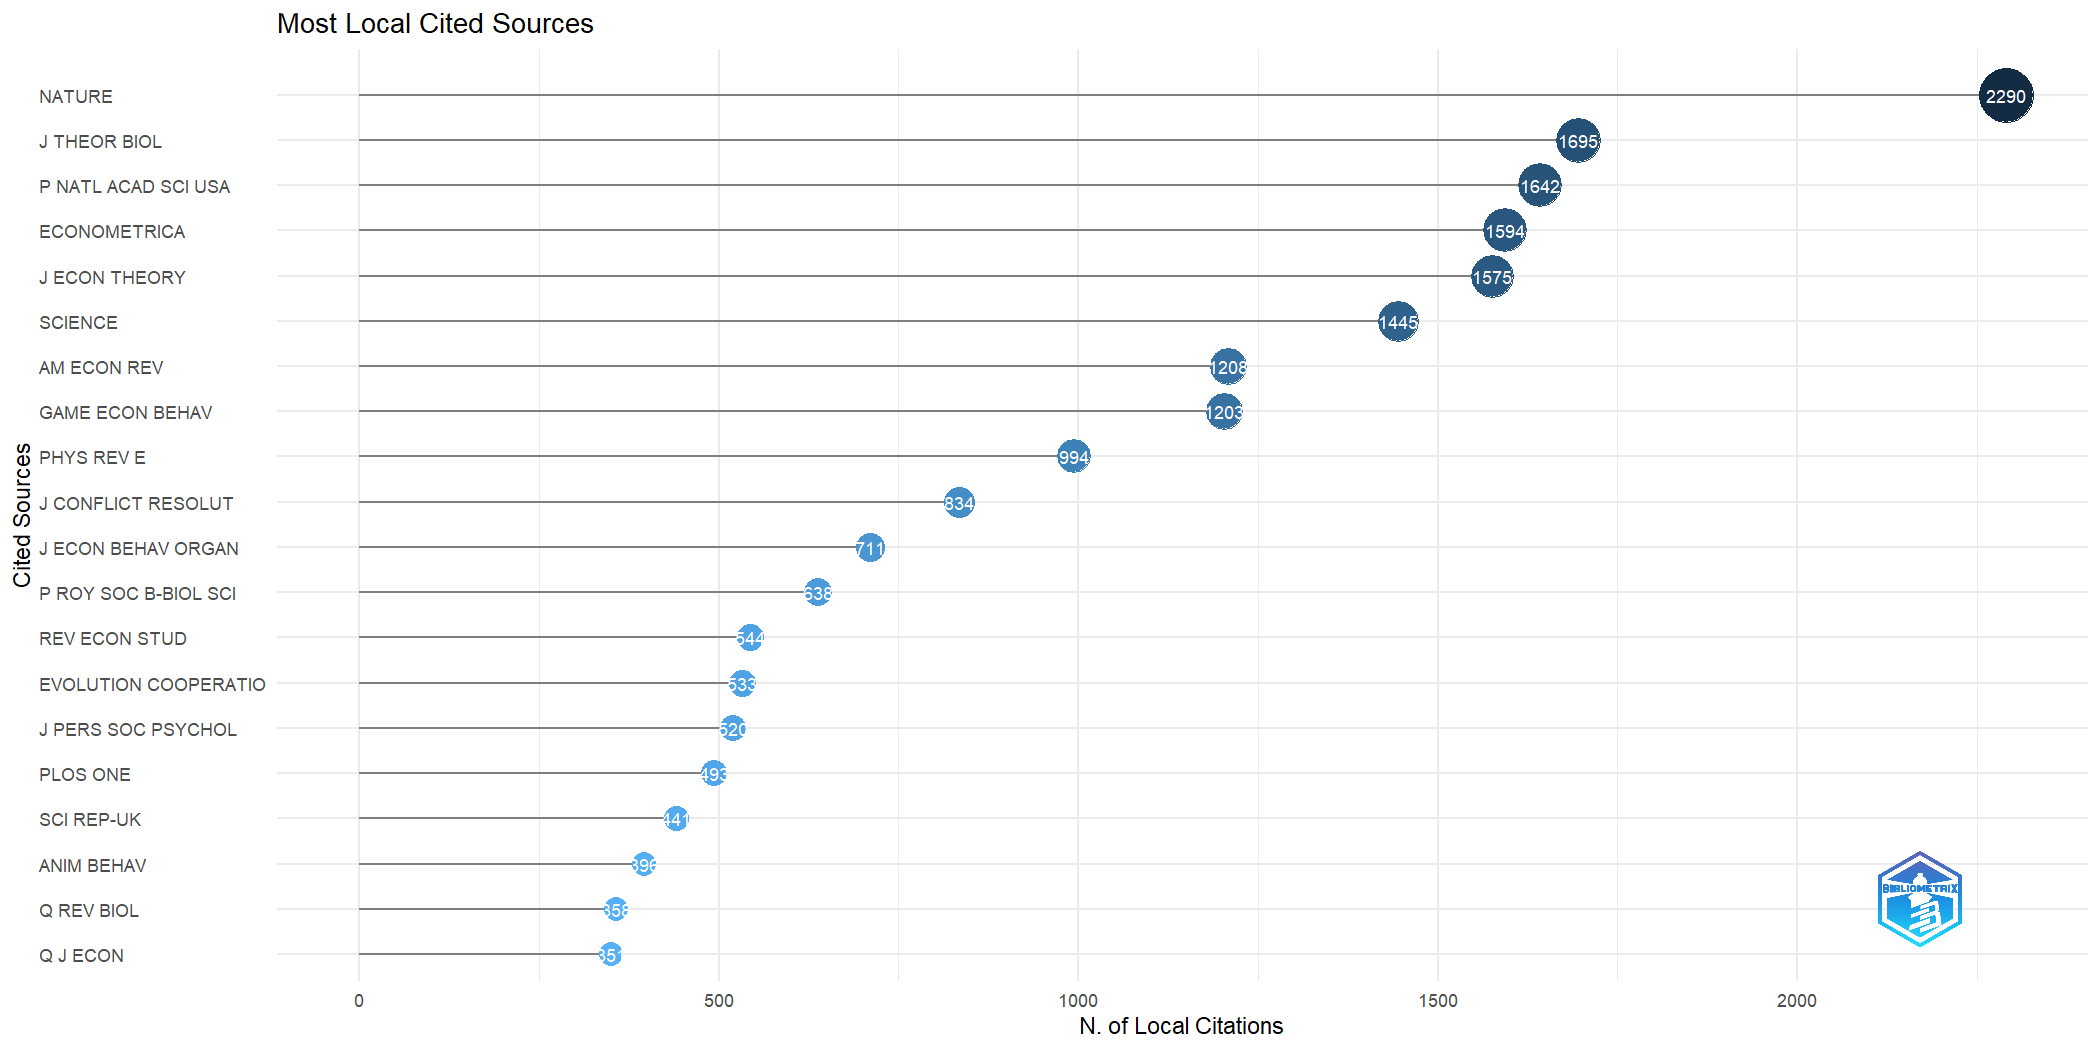
\includegraphics[width=1\textwidth]{exploratory-data-analysis/jvcalassio/PesqBibliogr/PrisonersDilemma/WoS-20221201/Dataset/MostLocalCitedSources-2022-12-03.png}
    \caption{Revistas mais relevantes no  \dataset\ PD@jvcalassio, conforme a soma de citações aos artigos no \dataset.}
    \label{fig:PD@jvcalassio:Most-Local-Cited-Sources(from-Reference-Lists).png}
\end{figure}

\subsection{Lei de Bradford}

Conforme podemos visualizar na figura \ref{fig:PD@jvcalassio:Bradfords-Law.png}, a fonte mais relevante nesse tema é o \textit{Journal of Theoretical Biology}, se utilizarmos como critério a Lei de Bradford.

\begin{figure}
    \centering
    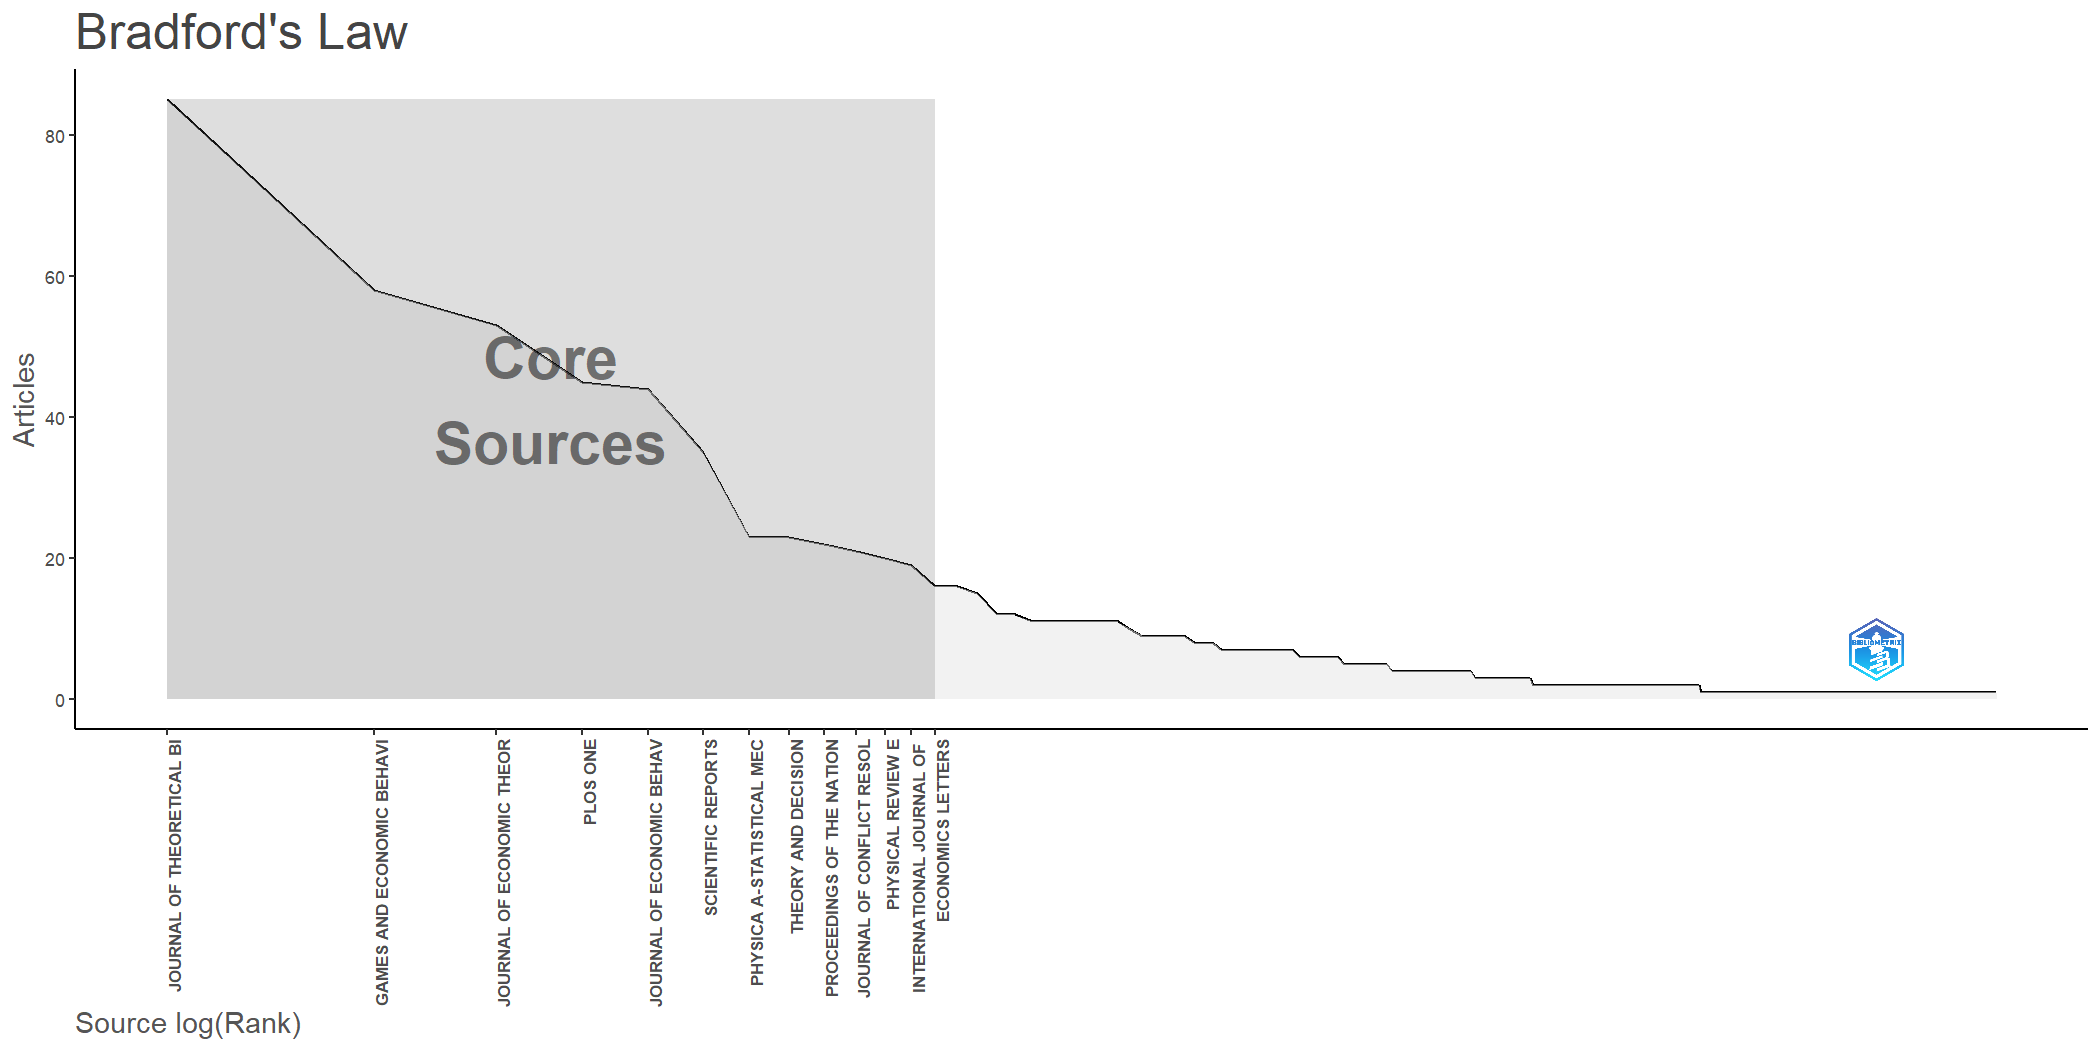
\includegraphics[width=1\textwidth]{exploratory-data-analysis/jvcalassio/PesqBibliogr/PrisonersDilemma/WoS-20221201/Dataset/BradfordLaws-2022-12-03.png}
    \caption{Revistas mais relevantes no  \dataset\ PD@jvcalassio, conforme a Lei de Bradford.}
    \label{fig:PD@jvcalassio:Bradfords-Law.png}
\end{figure}

\subsection{Medidas de Impacto das fontes}

Os já apresentados índices H, G e M também podem ser utilizados para medir a relevância das fontes:

\subsubsection{Índice H}

O índice H indica que a revista de maior impacto é o \textit{Journal of Theoretical Biology}, conforme mostra a figura \ref{fig:PD@jvcalassio:H-Index-Source-Local-Impact.png}.

\begin{figure}
    \centering
    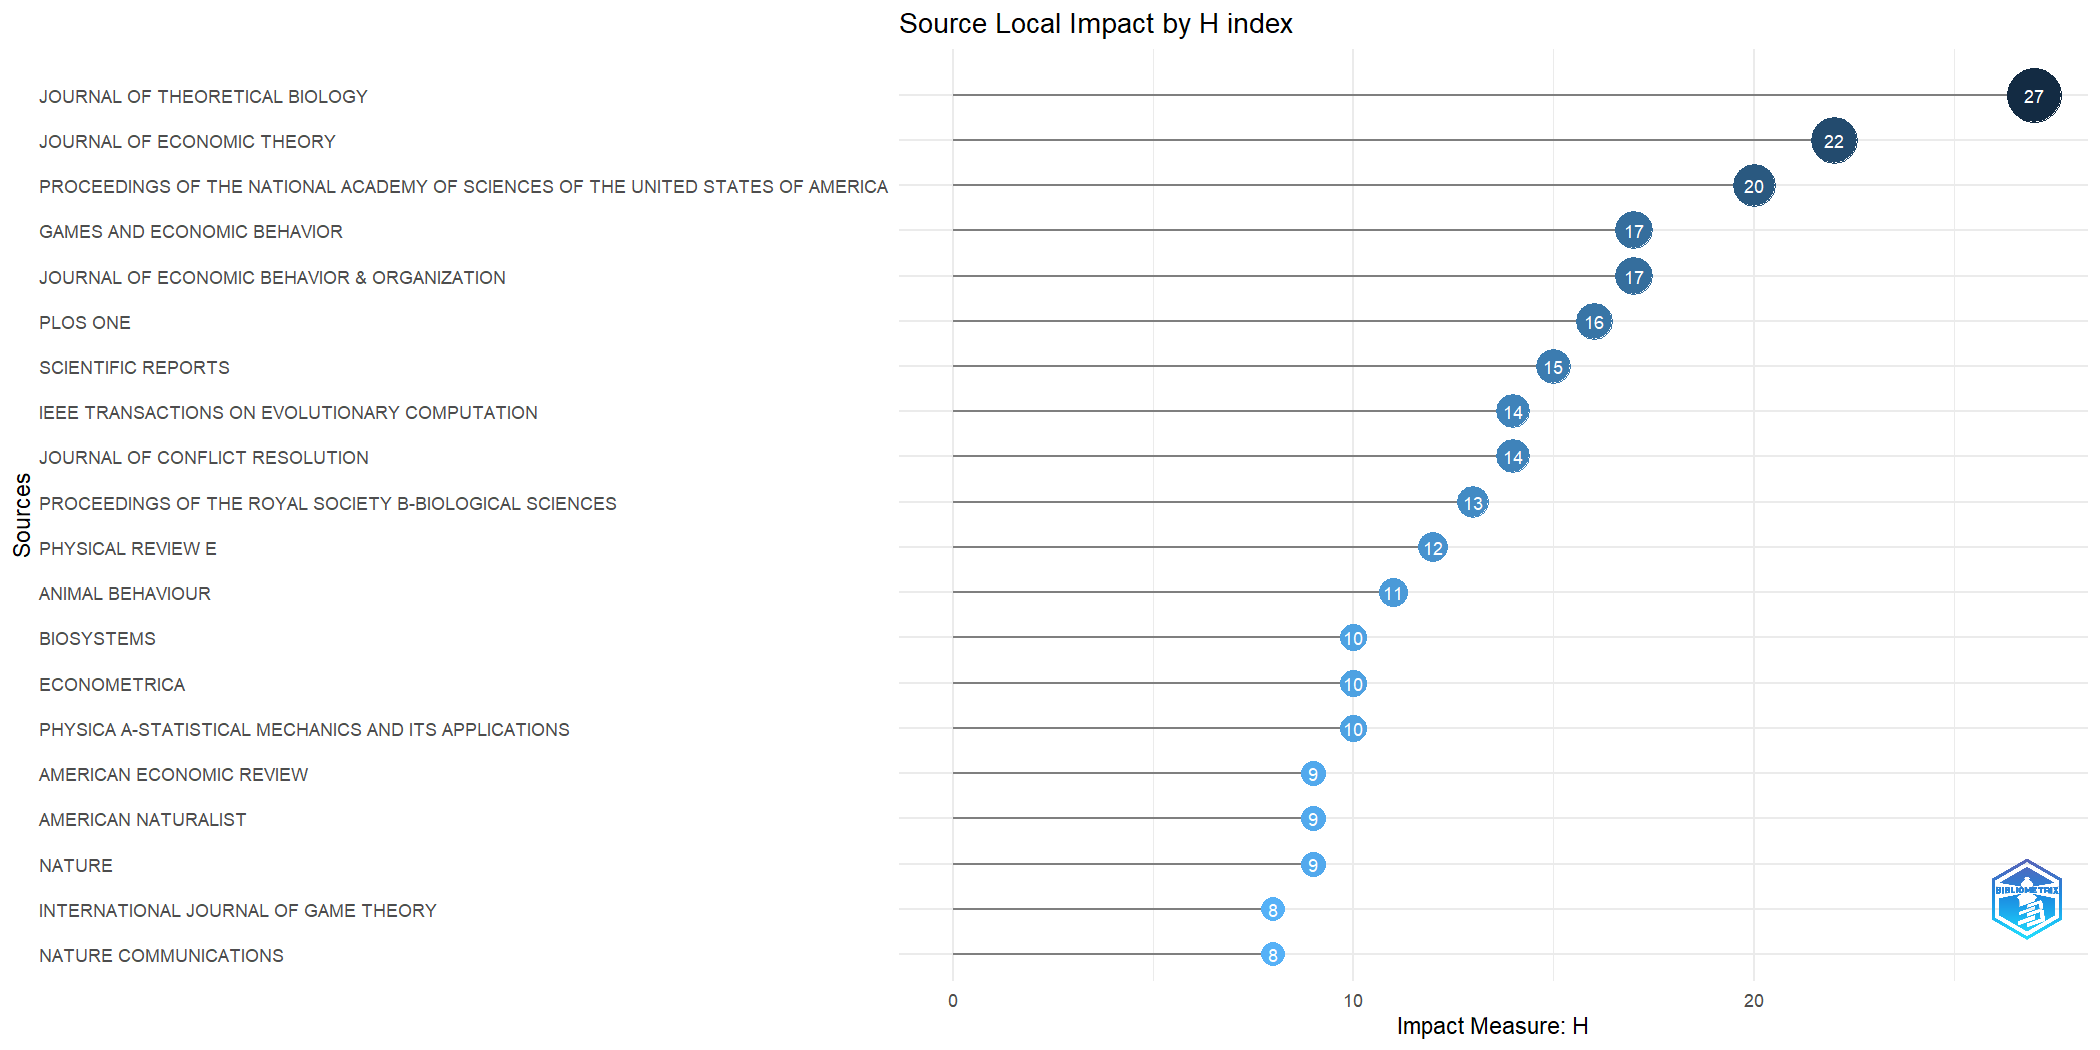
\includegraphics[width=1\textwidth]{exploratory-data-analysis/jvcalassio/PesqBibliogr/PrisonersDilemma/WoS-20221201/Dataset/SourceImpactH-2022-12-03.png}
    \caption{Revistas de maior impacto no  \dataset\ PD@jvcalassio,  conforme o índice H.}
    \label{fig:PD@jvcalassio:H-Index-Source-Local-Impact.png}
\end{figure}


\subsubsection{Índice G}

O índice G indica que a revista de maior impacto é o \textit{Journal of Economic Theory}, conforme mostra a figura \ref{fig:PD@jvcalassio:G-Index-Source-Local-Impact.png}.

\begin{figure}
    \centering
    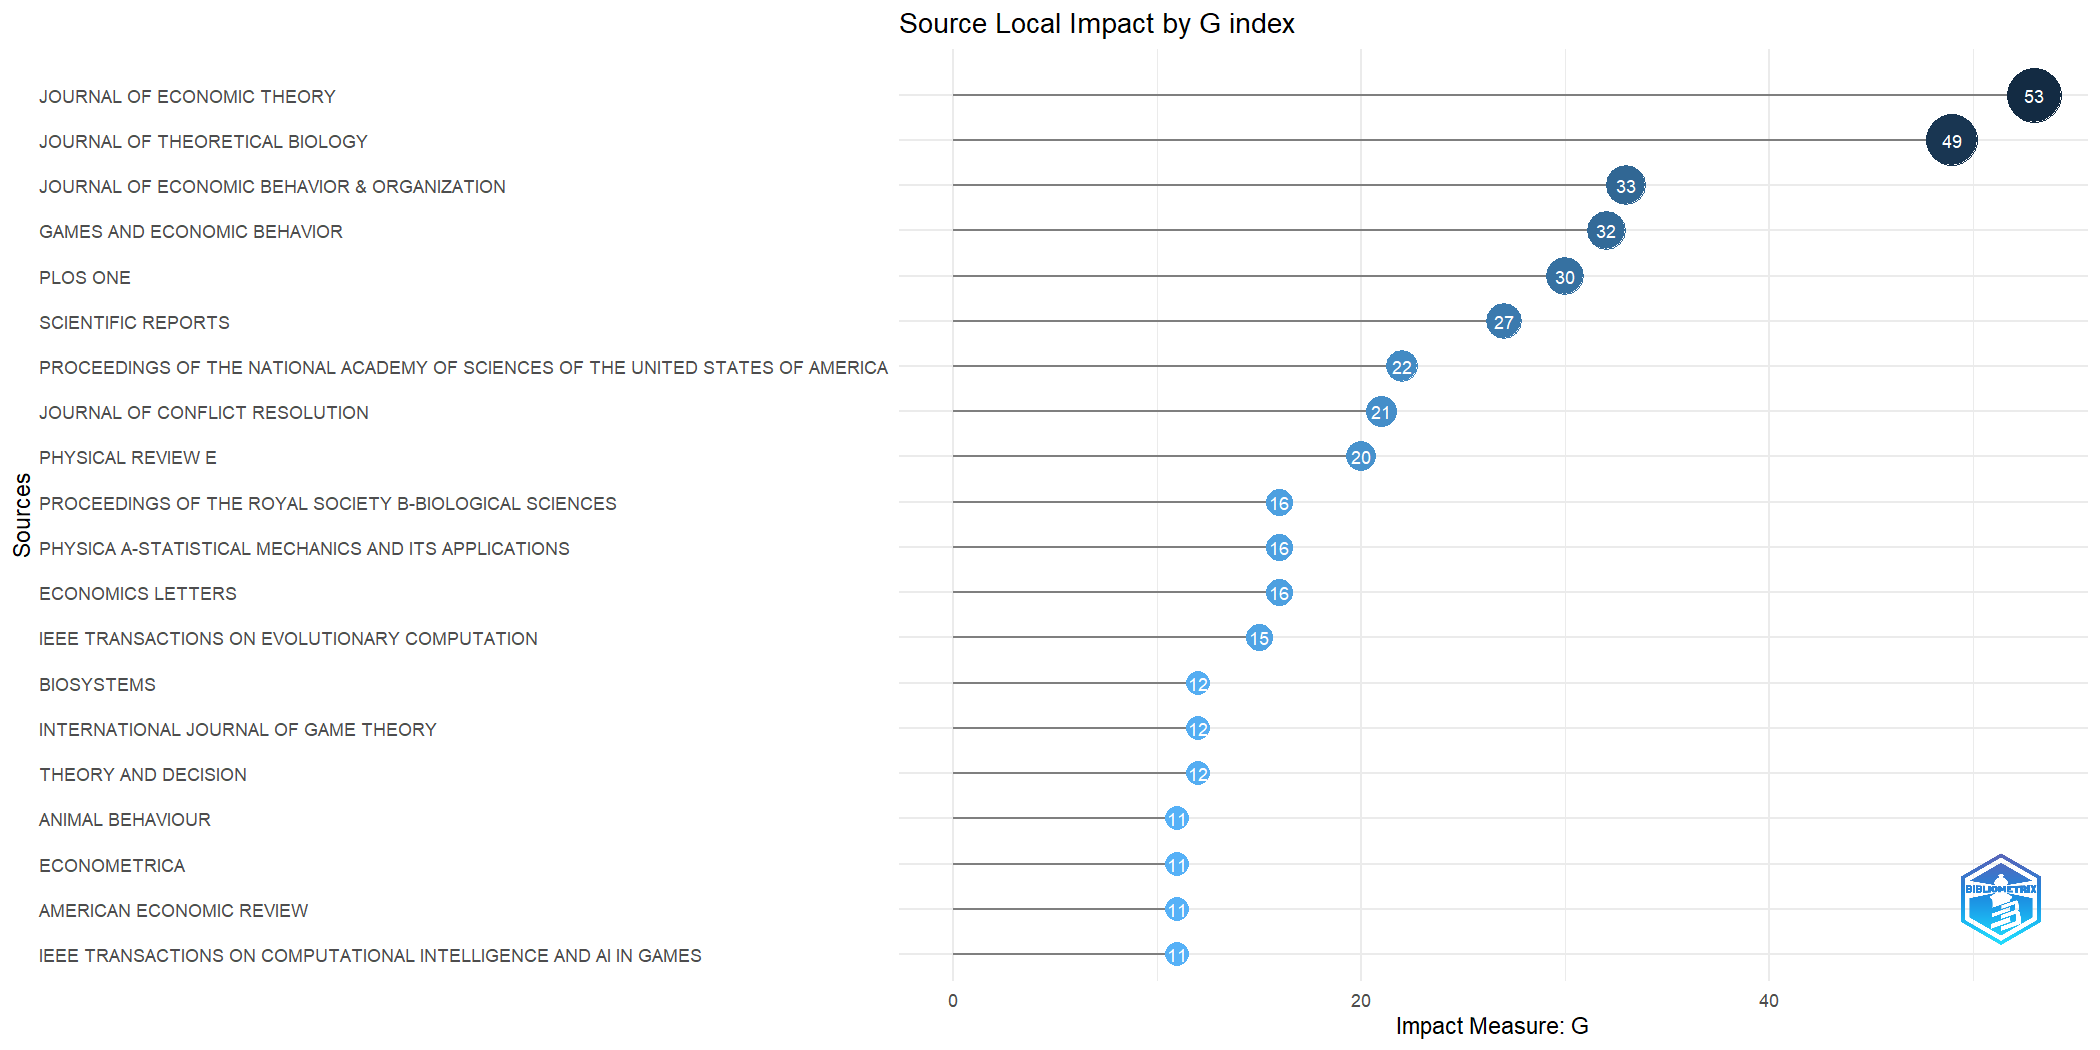
\includegraphics[width=1\textwidth]{exploratory-data-analysis/jvcalassio/PesqBibliogr/PrisonersDilemma/WoS-20221201/Dataset/SourceImpactG-2022-12-03.png}
    \caption{Revistas de maior impacto no  \dataset\ PD@jvcalassio,  conforme o índice G.}
    \label{fig:PD@jvcalassio:G-Index-Source-Local-Impact.png}
\end{figure}

\subsubsection{Índice M}

O índice M indica que a revista de maior impacto é a \textit{Scientific Reports}, conforme mostra a figura \ref{fig:PD@jvcalassio:M-Index-Source-Local-Impact.png}.

\begin{figure}
    \centering
    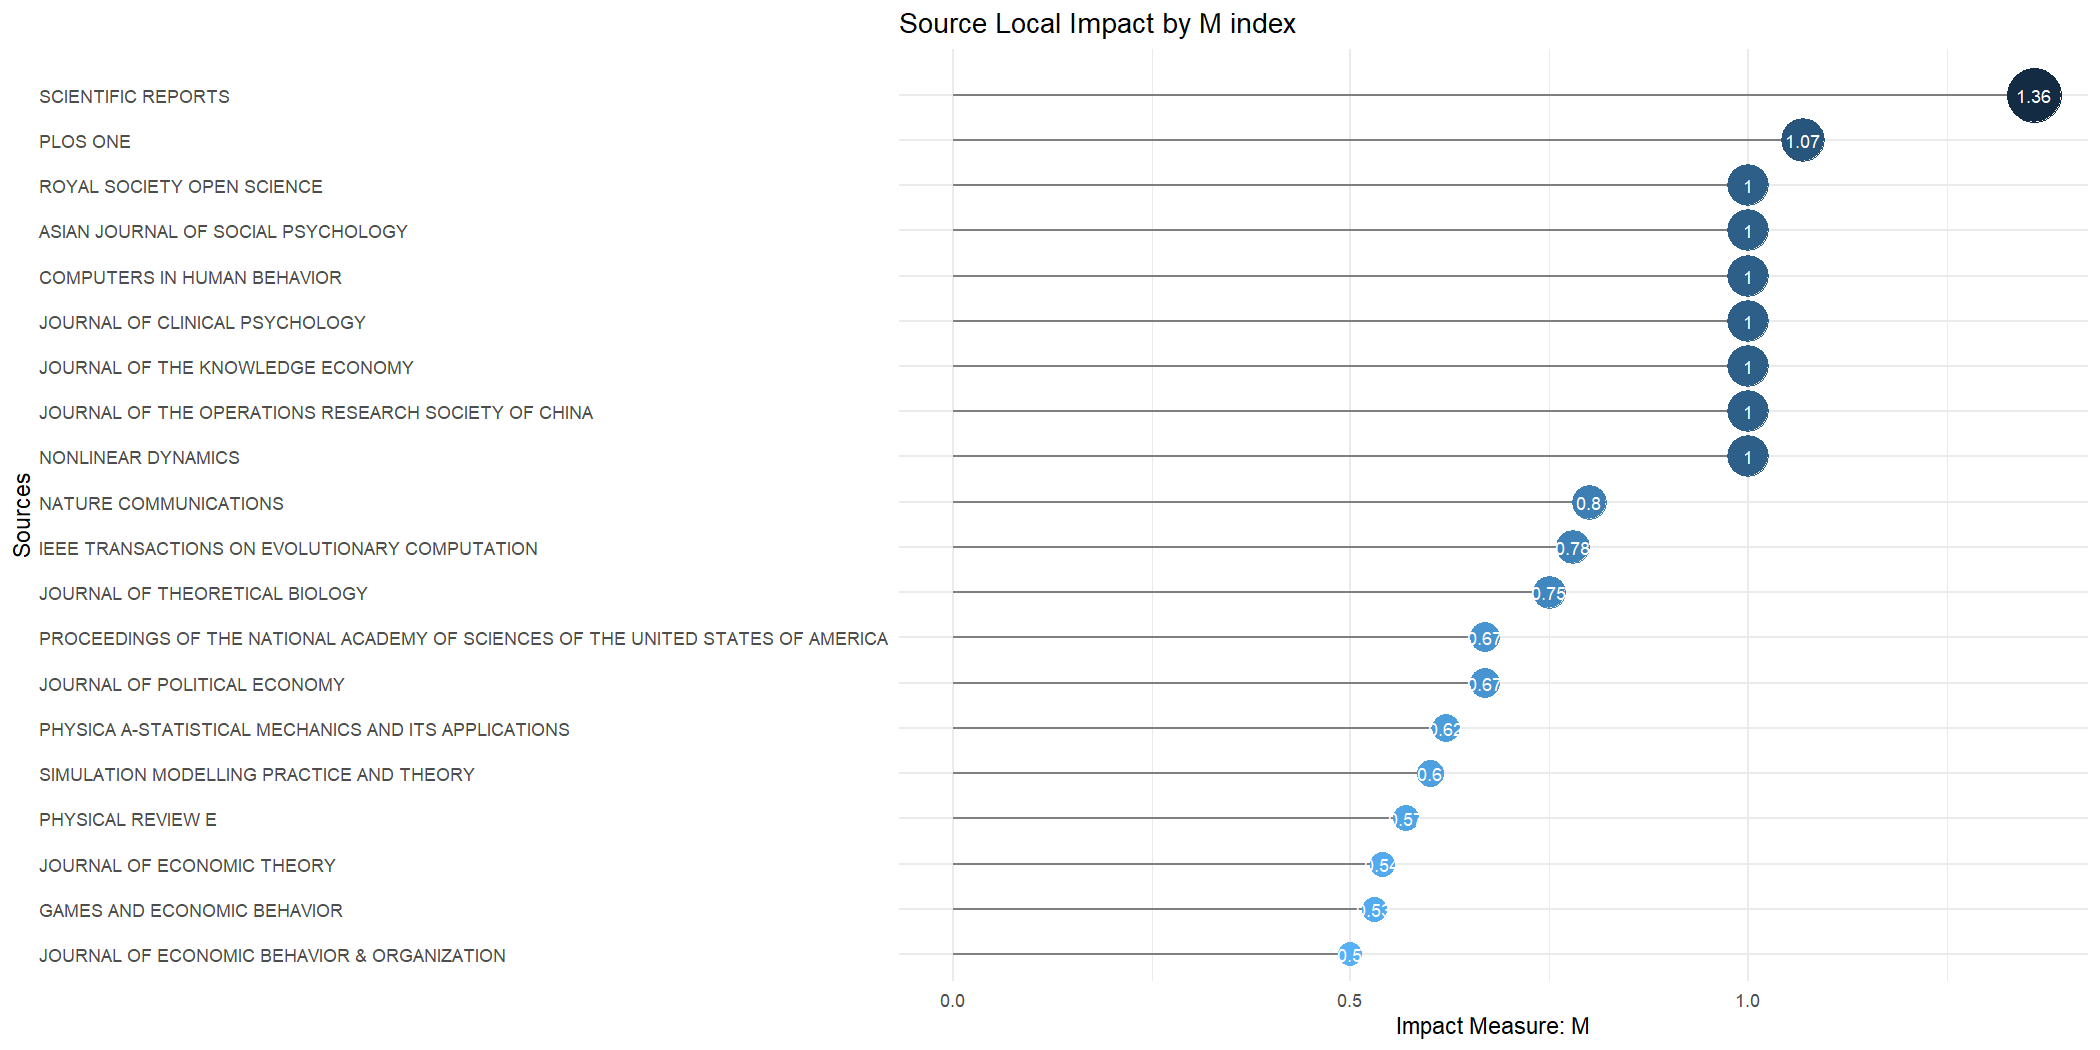
\includegraphics[width=1\textwidth]{exploratory-data-analysis/jvcalassio/PesqBibliogr/PrisonersDilemma/WoS-20221201/Dataset/SourceImpactM-2022-12-03.png}
    \caption{Revistas de maior impacto no  \dataset\ PD@jvcalassio,  conforme o índice M.}
    \label{fig:PD@jvcalassio:M-Index-Source-Local-Impact.png}
\end{figure}

\subsection{Dinâmica de publicação nas fontes}

E à partir da figura \ref{fig:PD@jvcalassio:Source-Dynamics.png}, podemos visualizar quais revistas tiveram o maior volume de publicações no tema ao longo do tempo.

\begin{figure}
    \centering
    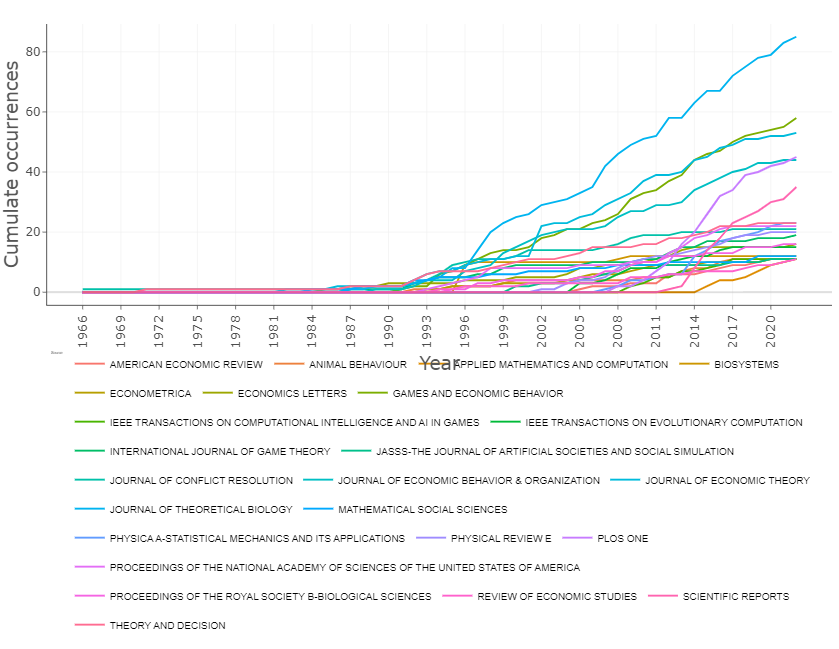
\includegraphics[width=1\textwidth]{exploratory-data-analysis/jvcalassio/PesqBibliogr/PrisonersDilemma/WoS-20221201/Dataset/SourceDynamics-2022-12-03.png}
    \caption{Revistas com maior volume de publicações no tema no  \dataset\ PD@jvcalassio, ao longo do tempo.}
    \label{fig:PD@jvcalassio:Source-Dynamics.png}
\end{figure}

\subsection{Estrutura Conceitual do Conhecimento}

O Conhecimento científico é um fenômeno complexo que emerge a partir da agregação memética de termos e palavras, que representam conceitos e ideias, que se organizam em tópicos, temas, e que evoluem ao longo do tempo (ver \url{https://en.wikipedia.org/wiki/Memetics}).

A estrutura conceitual do conhecimento pode ser produzida pela análise de relacionamento estabelecidos entre esses termos. O bibliometrix apresenta um conjunto de técnicas para evidenciar essa estrutura conceitual, e que se organizam em dois grupos:
\begin{description}
    \item [Métricas em rede] que usam grafos para representar relacionamentos entre termos, evidenciando, por meio de métricas de análise de redes sociais, como o conhecimento conceitualmente se organiza.
    \item [Análise Fatorial] Que emprega métricas de redução da dimensionalidade, para explorar, usualmente em mapas bidimensionais, como os termos e palavras se relacionam. 
\end{description}

\subsubsection{Métricas aplicadas a grafos (redes)}

\paragraph{Redes de Coocorrências}

As redes de coocorrências apresentam importantes padrões que se formam nas publicações, e podem revelar a estrutura conceitual de uma área do conhecimento.

No Biblioshiny três tipos de redes podem ser geradas baseadas em coocorrência:
\begin{itemize}
    \item Rede de palavras-chave, revelando quais são as palavras-chave mais comumente usadas simultaneamente em um documento, revelando os grupos de conceitos-chave. As palavras-chave podem ser as originalmente usadas pelos autores (mais variáveis) ou as usadas durante a indexação (mais padronizadas);
    \item Redes de palavras (ngramas) usadas de forma simultânea nos títulos dos artigos;
    \item Redes de palavras (ngramas) usadas de forma simultânea nos resumos dos artigos.
\end{itemize}

A figura \ref{fig:PD@jvcalassio:Co-occurrence-Network} apresenta as 50 palavras-chave padronizadas (Keyword Plus) mais evidentes, clusterizadas pela coocorrência em documentos, no  \dataset\ PD@jvcalassio.

\begin{figure}
    \centering
    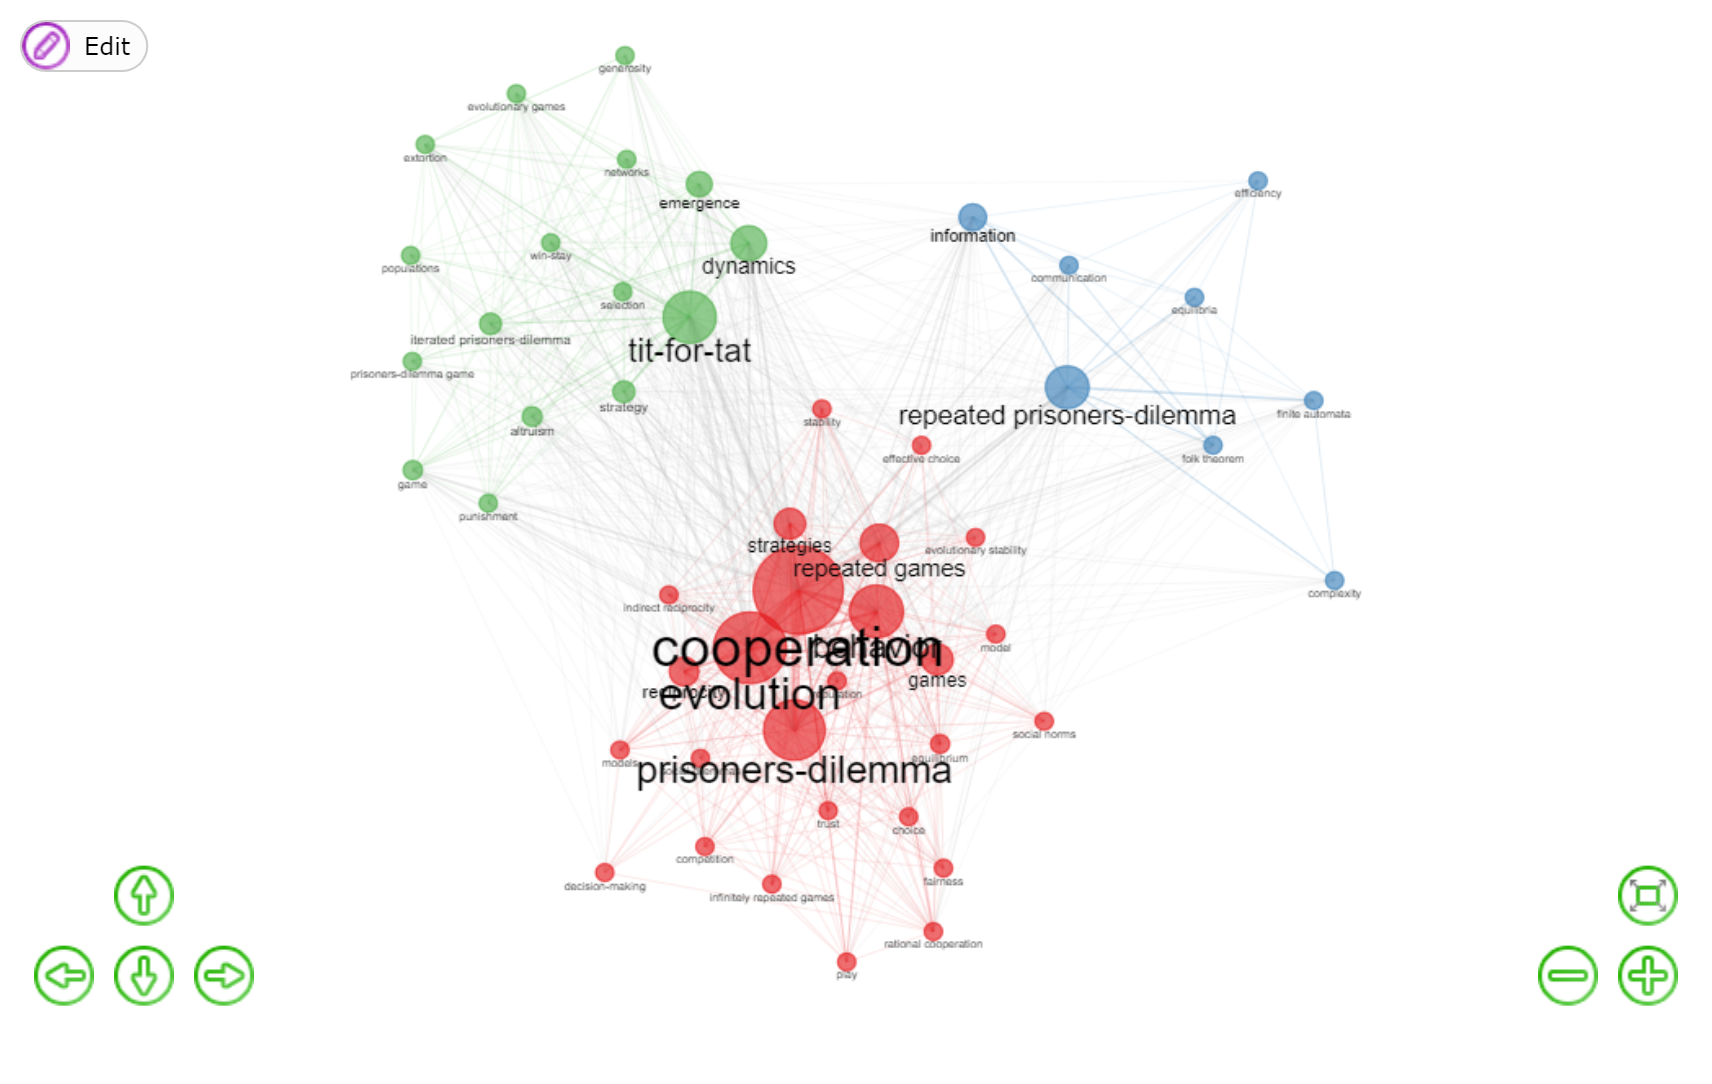
\includegraphics[width=1\textwidth]{exploratory-data-analysis/jvcalassio/PesqBibliogr/PrisonersDilemma/WoS-20221201/Dataset/Co-occurrence-Network-2022-12-03.png}
    \caption{50 palavras-chave mais evidentes, clusterizadas pela coocorrência em documentos, no  \dataset\ PD@jvcalassio.}
    \label{fig:PD@jvcalassio:Co-occurrence-Network}
\end{figure}

A fim de compreender como essas palavras ocorrem em conjunto, cada cluster podem ser analisado individualmente, como evidenciam as figuras \ref{fig:PD@jvcalassio:Co-occurrence-Network:Cluster1}, \ref{fig:PD@jvcalassio:Co-occurrence-Network:Cluster2} e \ref{fig:PD@jvcalassio:Co-occurrence-Network:Cluster3}.

\begin{figure}
    \centering
    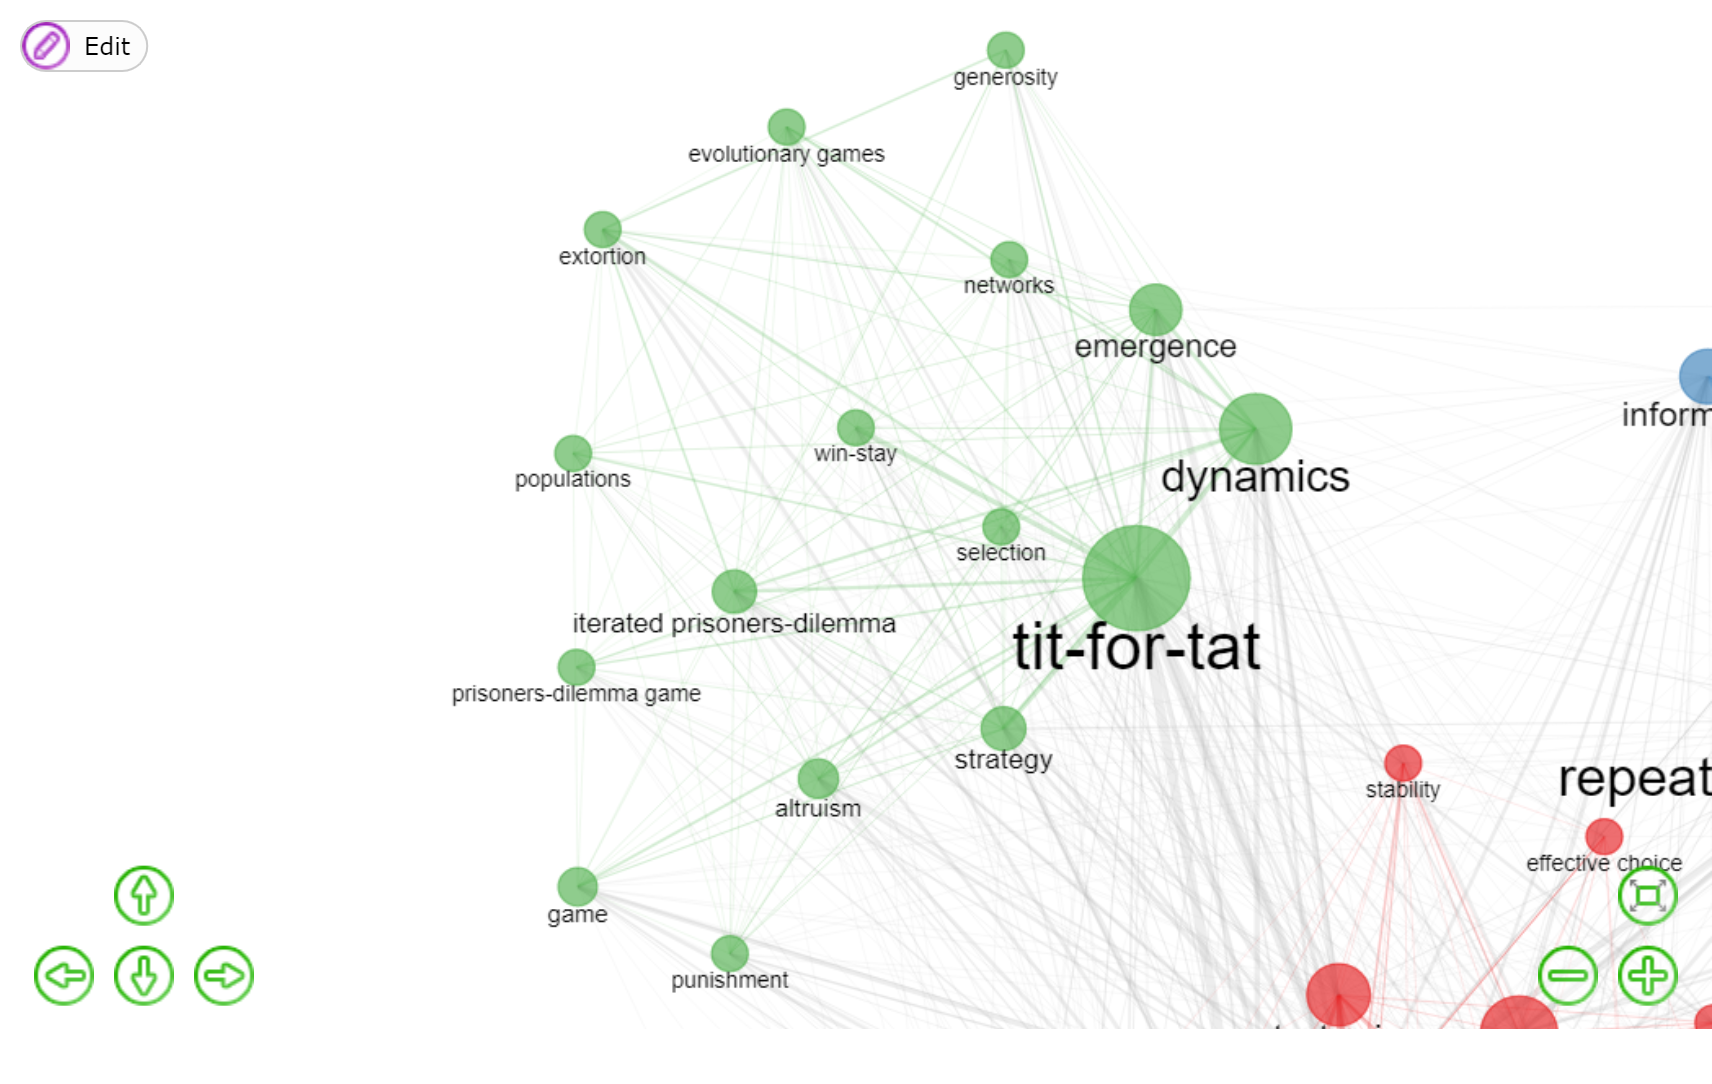
\includegraphics[width=1\textwidth]{exploratory-data-analysis/jvcalassio/PesqBibliogr/PrisonersDilemma/WoS-20221201/Dataset/Cluster1-Co-occurrence-Network-2022-12-03.png}
    \caption{Detalhamento do cluster 1, na rede das 50 palavras-chave mais evidentes, clusterizadas pela coocorrência em documentos, no  \dataset\ PD@jvcalassio.}
    \label{fig:PD@jvcalassio:Co-occurrence-Network:Cluster1}
\end{figure}

\begin{figure}
    \centering
    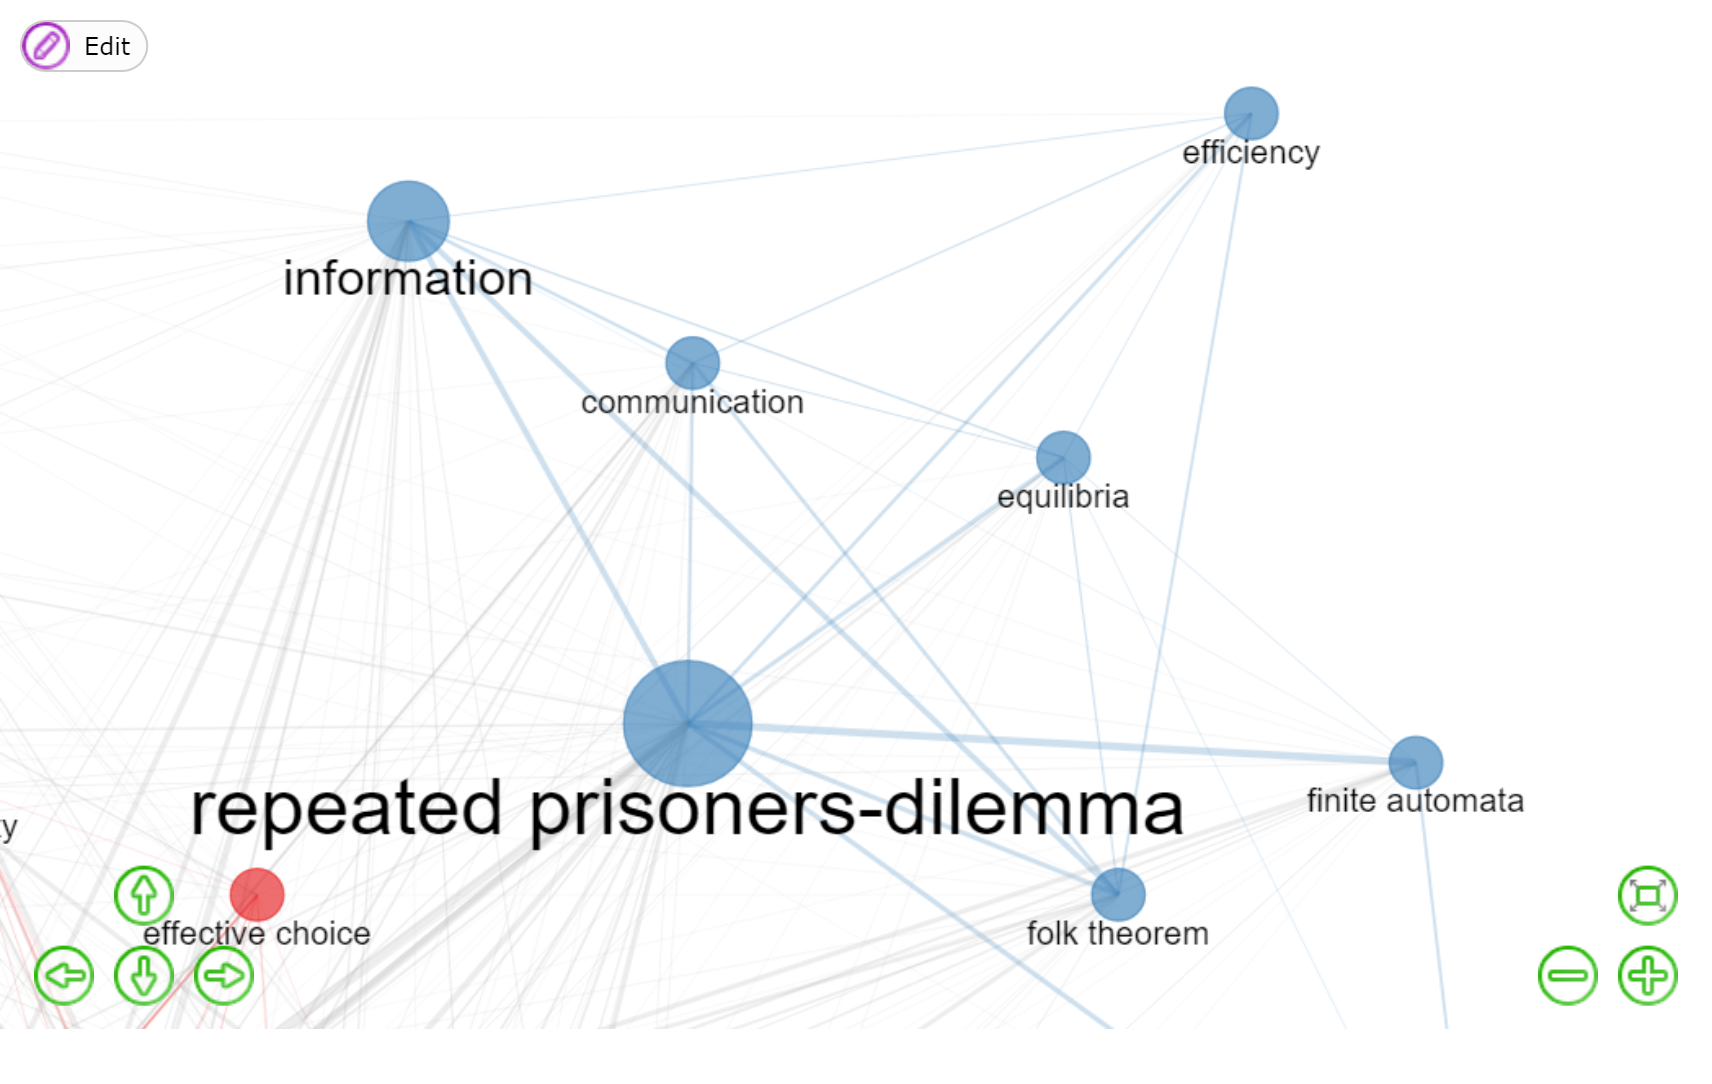
\includegraphics[width=1\textwidth]{exploratory-data-analysis/jvcalassio/PesqBibliogr/PrisonersDilemma/WoS-20221201/Dataset/Cluster2-Co-occurrence-Network-2022-12-03.png}
    \caption{Detalhamento do cluster 2, na rede das 50 palavras-chave mais evidentes, clusterizadas pela coocorrência em documentos, no  \dataset\ PD@jvcalassio.}
    \label{fig:PD@jvcalassio:Co-occurrence-Network:Cluster2}
\end{figure}

\begin{figure}
    \centering
    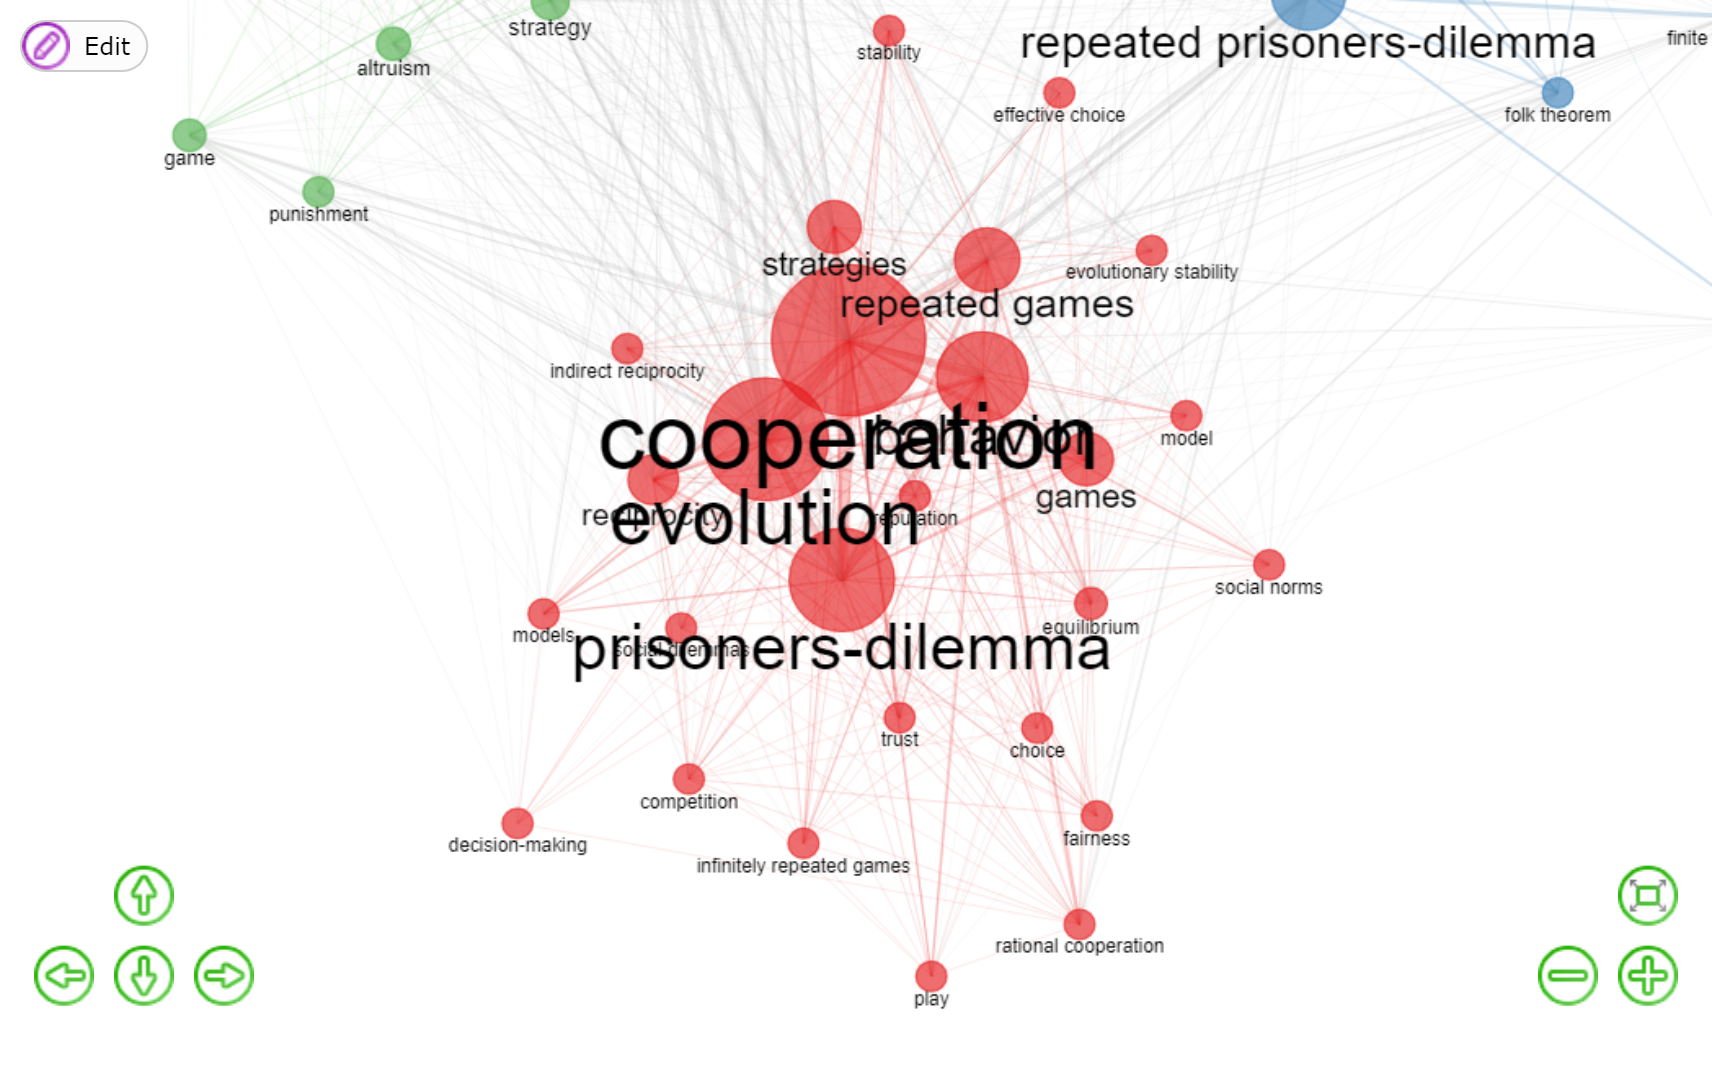
\includegraphics[width=1\textwidth]{exploratory-data-analysis/jvcalassio/PesqBibliogr/PrisonersDilemma/WoS-20221201/Dataset/Cluster3-Co-occurrence-Network-2022-12-03.png}
    \caption{Detalhamento do cluster 3, na rede das 50 palavras-chave mais evidentes, clusterizadas pela coocorrência em documentos, no  \dataset\ PD@jvcalassio.}
    \label{fig:PD@jvcalassio:Co-occurrence-Network:Cluster3}
\end{figure}

\paragraph{Mapas Temáticos}

O mapa temático pode ser visualizado na figura \ref{fig:PD@jvcalassio:ThematicMap}. Podemos observar que há cinco grandes temas.

\begin{figure}
    \centering
    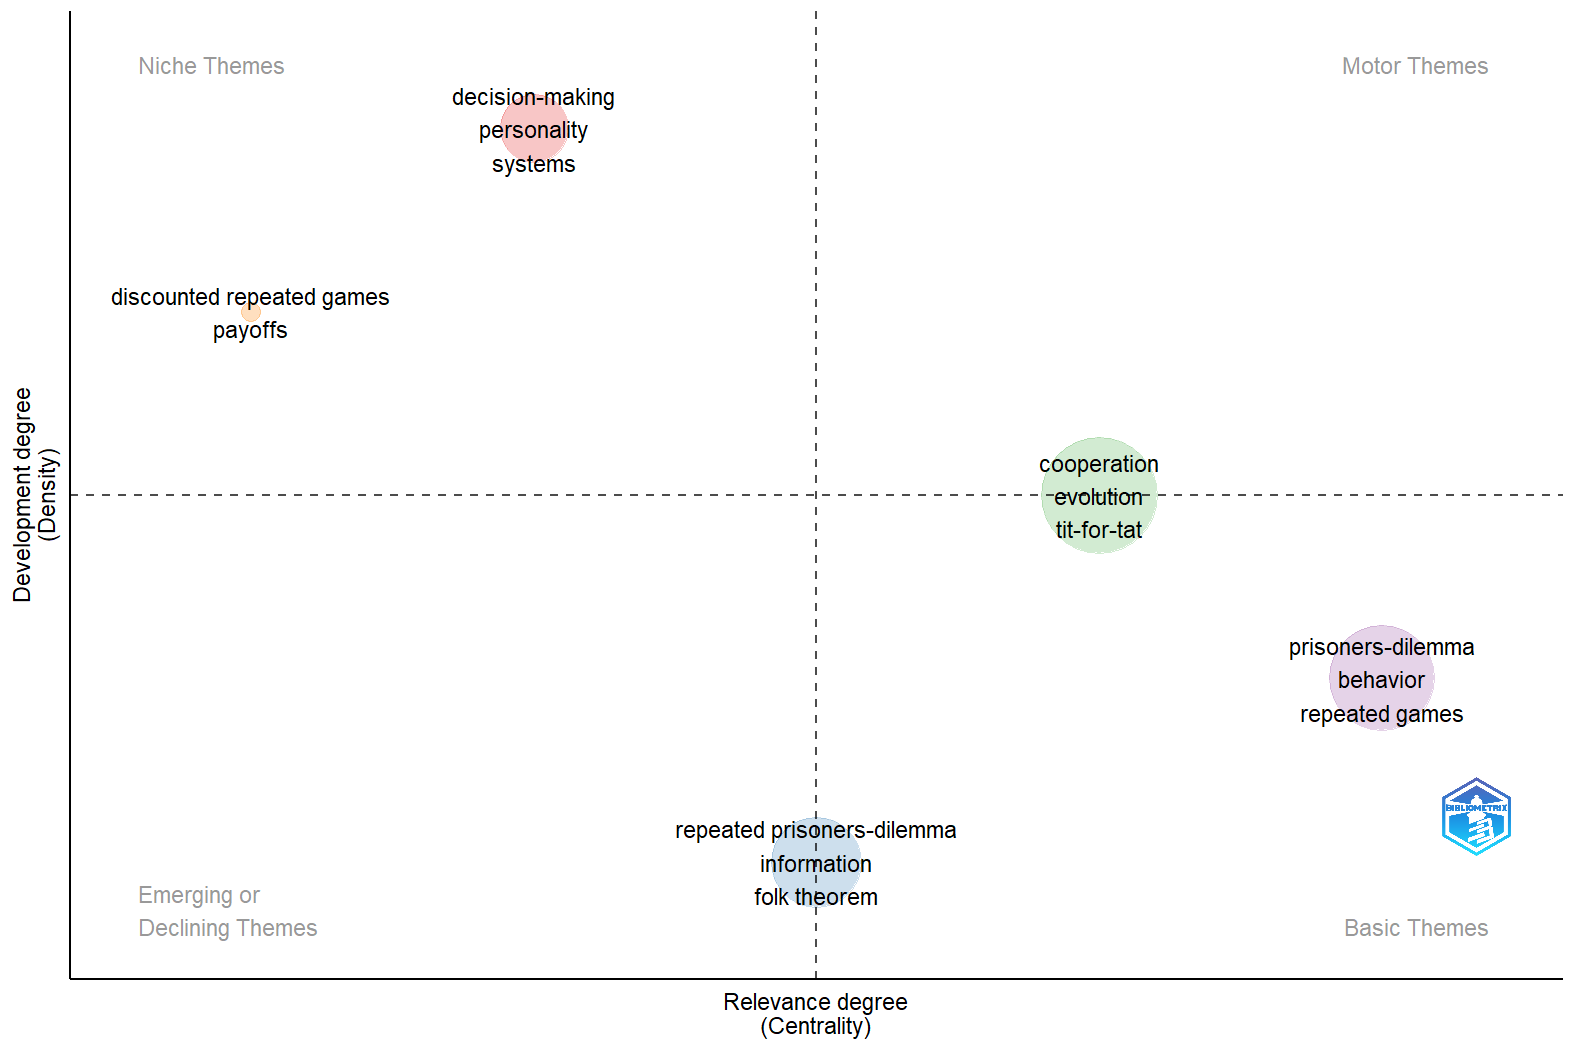
\includegraphics[width=0.9\textwidth]{exploratory-data-analysis/jvcalassio/PesqBibliogr/PrisonersDilemma/WoS-20221201/Dataset/ThematicMap-2022-12-03.png}
    \caption{Mapa temático do  \dataset\ PD@jvcalassio.}
    \label{fig:PD@jvcalassio:ThematicMap}
\end{figure}

\paragraph{Evolução Temática}

A evolução temática pode ser visualizada na figura \ref{fig:PD@jvcalassio:Thematic-Evolution}. Podemos observar que grande parte do foco temático se voltou para a cooperação.

\begin{figure}
    \centering
    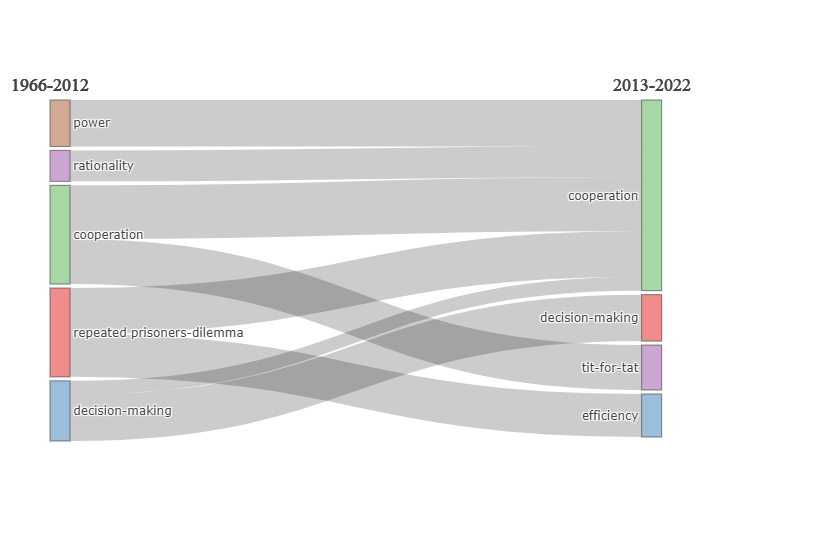
\includegraphics[width=1\textwidth]{exploratory-data-analysis/jvcalassio/PesqBibliogr/PrisonersDilemma/WoS-20221201/Dataset/ThematicEvolution-2022-12-03.png}
    \caption{Evolução temática do  \dataset\ PD@jvcalassio.}
    \label{fig:PD@jvcalassio:Thematic-Evolution}
\end{figure}

\subsubsection{Métricas de redução da dimensionalidade (Análise Fatorial)}

No mapa fatorial da figura \ref{fig:PD@jvcalassio:FactorialAnalysis-MCA-FactorialMap}, podemos observar que aparentemente existem dois grandes temas conceituais estudados dentro do tema dilema do prisioneiro iterativo.

\begin{figure}
    \centering
    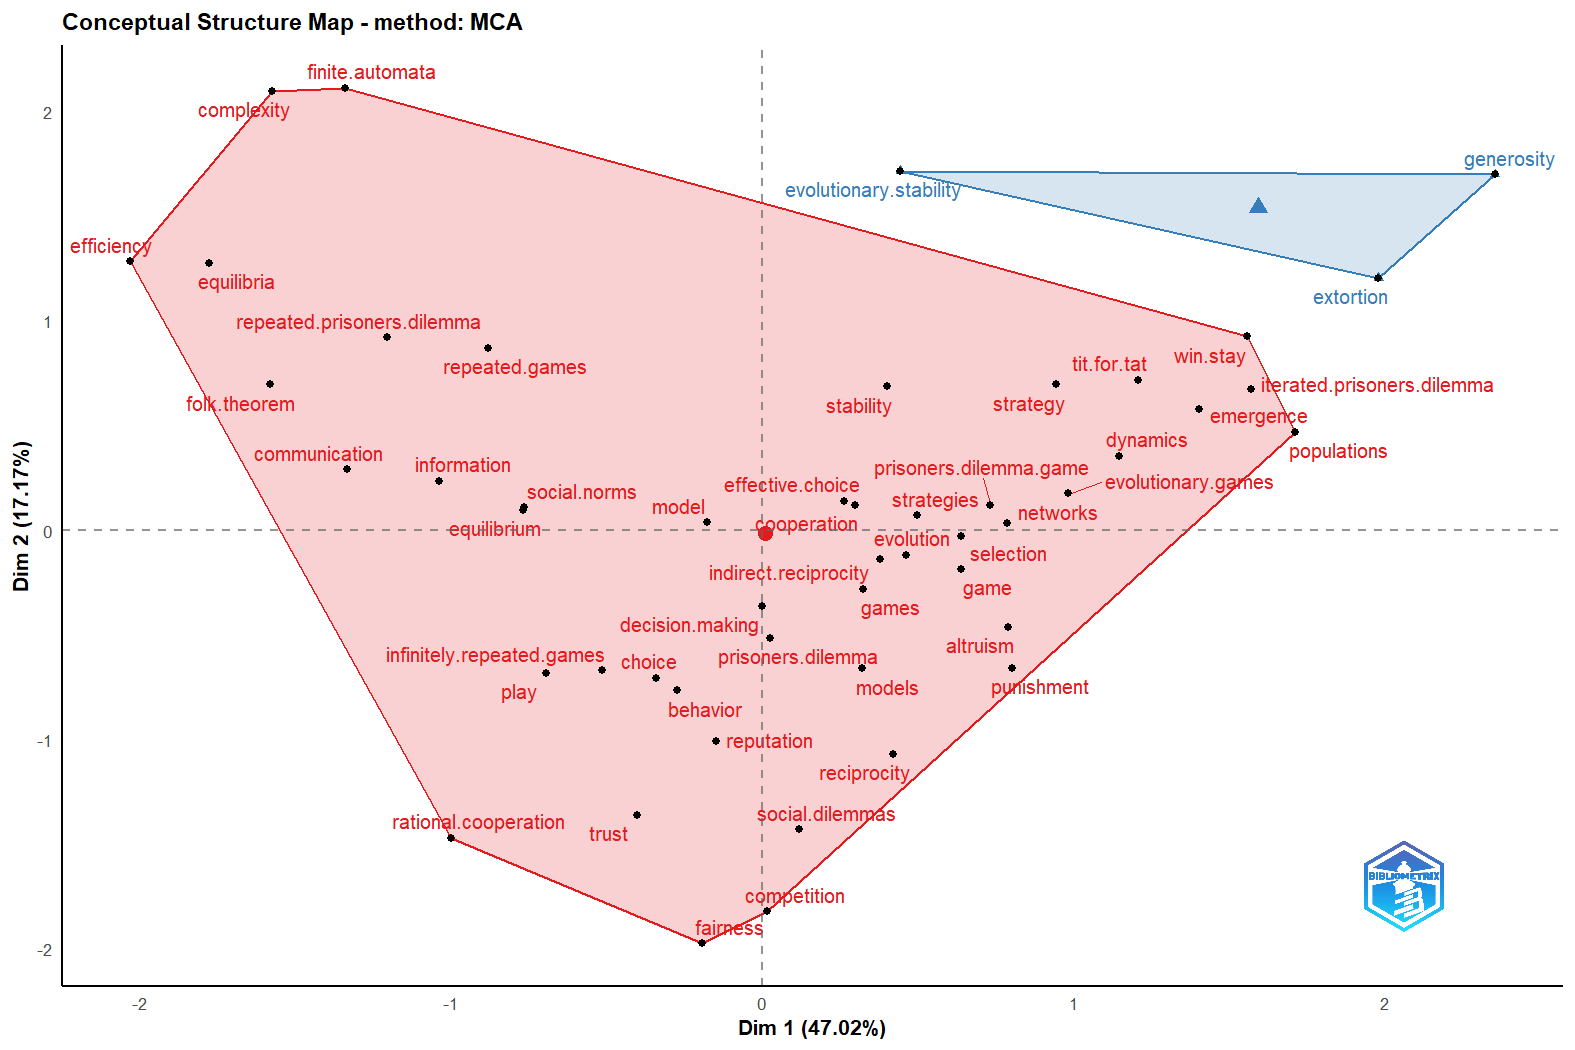
\includegraphics[width=0.9\textwidth]{exploratory-data-analysis/jvcalassio/PesqBibliogr/PrisonersDilemma/WoS-20221201/Dataset/FactorialMap-2022-12-03.png}
    \caption{Dimensões de variabilidade mais relevantes, nas palavras-chave do  \dataset\ PD@jvcalassio.}
    \label{fig:PD@jvcalassio:FactorialAnalysis-MCA-FactorialMap}
\end{figure}

\begin{figure}
    \centering
    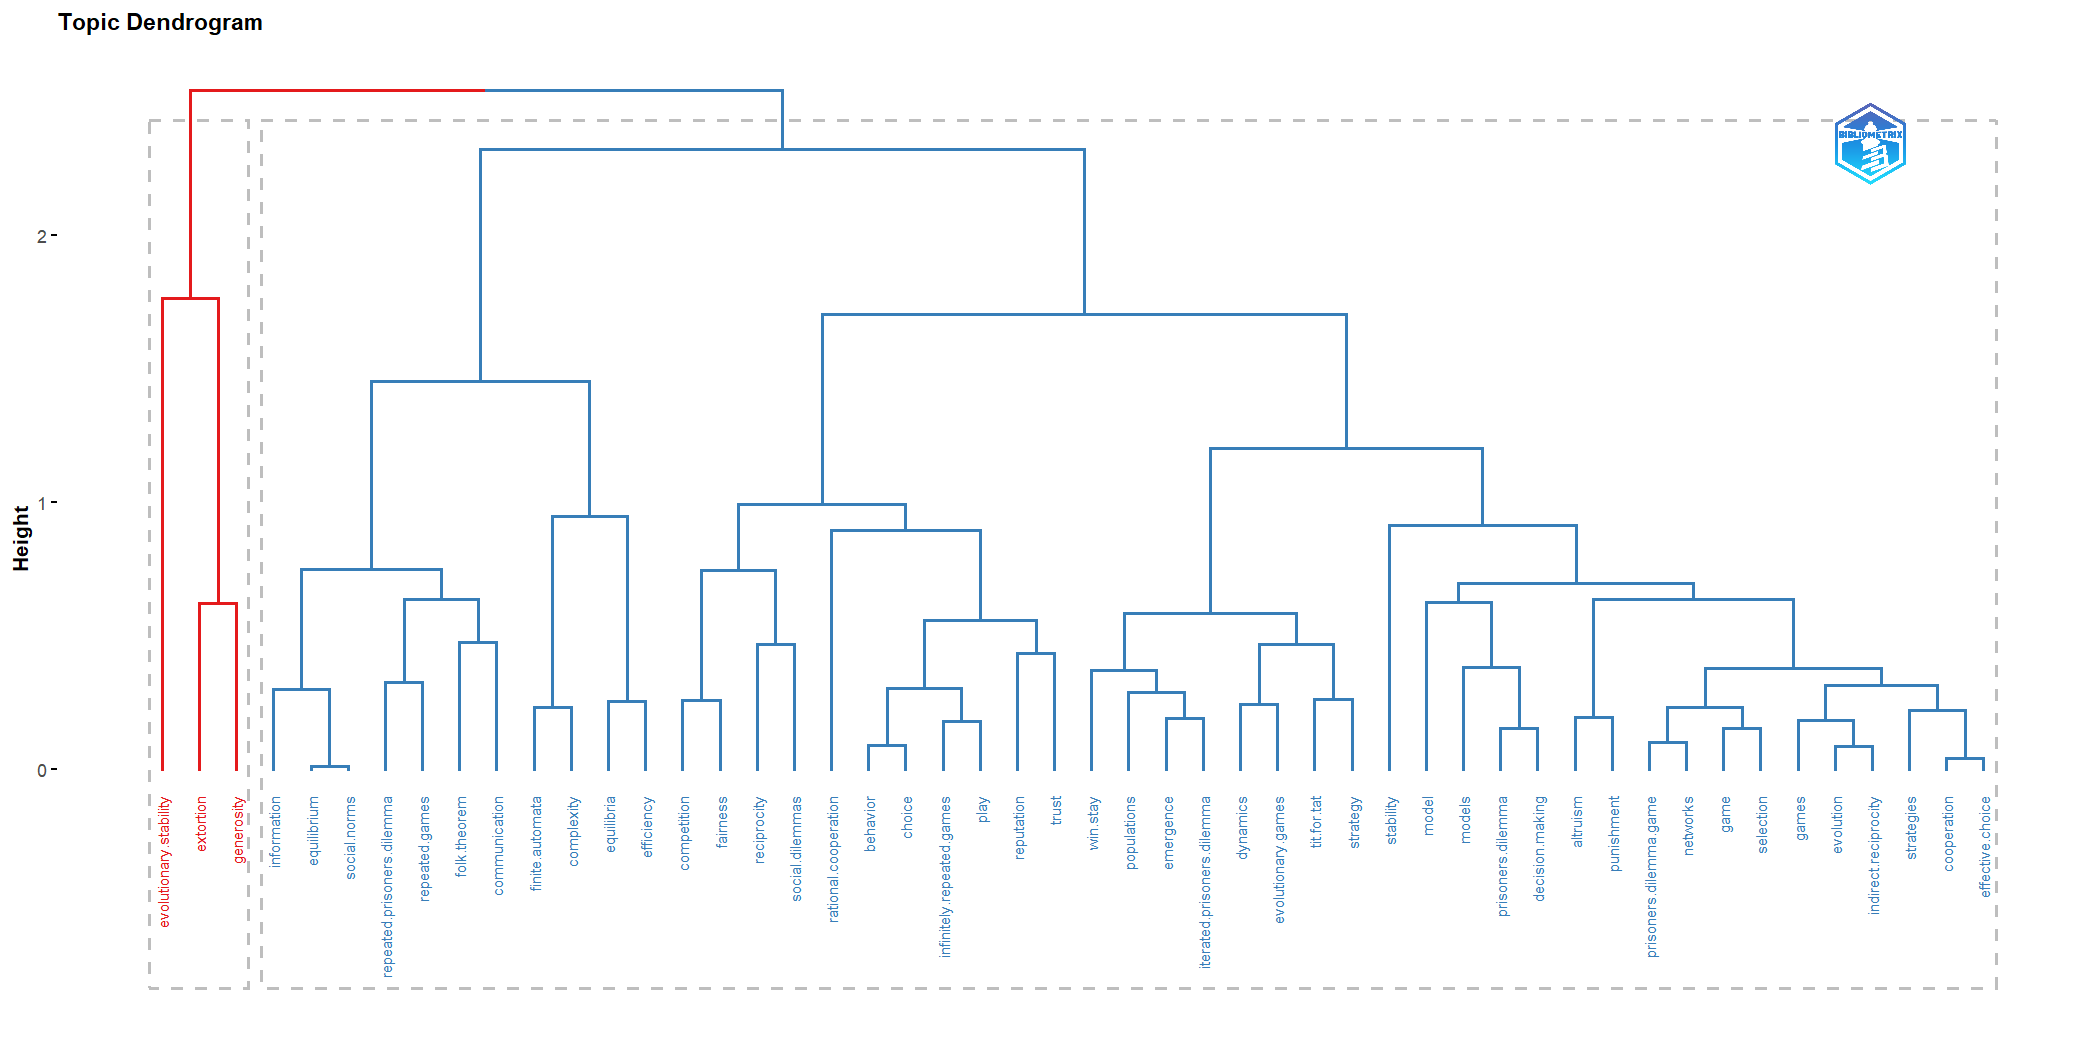
\includegraphics[width=1\textwidth]{exploratory-data-analysis/jvcalassio/PesqBibliogr/PrisonersDilemma/WoS-20221201/Dataset/Dendrogram-2022-12-03.png}
    \caption{Dendograma das dimensões de variabilidade mais relevantes, nas palavras-chave do  \dataset\ PD@jvcalassio.}
    \label{fig:PD@jvcalassio:FactorialAnalysis-MCA-Dendrogram}
\end{figure}

\begin{figure}
    \centering
    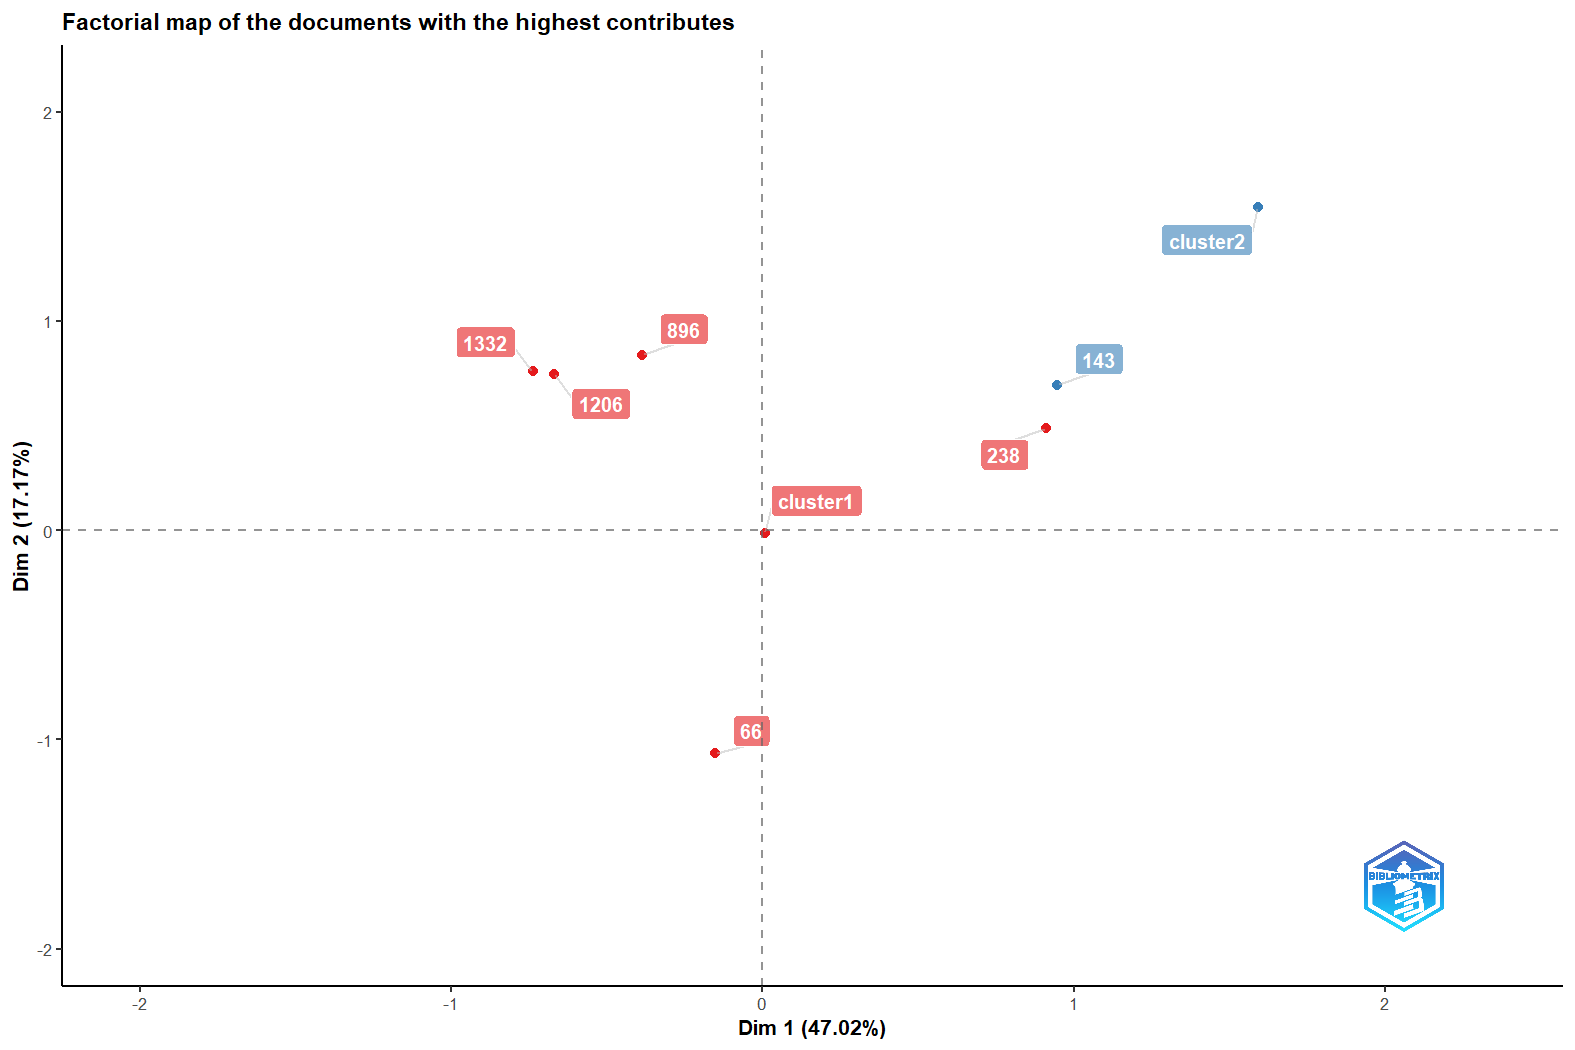
\includegraphics[width=0.7\textwidth]{exploratory-data-analysis/jvcalassio/PesqBibliogr/PrisonersDilemma/WoS-20221201/Dataset/MostContribDocuments-2022-12-03.png}
    \caption{Documentos que mais contribuíram para determinar das dimensões de variabilidade mais relevantes, nas palavras-chave do  \dataset\ PD@jvcalassio.}
    \label{fig:PD@jvcalassio:FactorialAnalysis-MCA-MostContribDocuments}
\end{figure}

\subsection{Estrutura Intelectual do Conhecimento}

Conhecimento científico é produzido por processos intelectuais onde autores de trabalho escolhem deliberadamente referenciar trabalhos de outros, por meio de documentos publicados, que são encaminhados para publicações em fontes de informação de sua escolha, e que evoluem ao longo do tempo.

O Bibliometrix permite exploração da estrutura intelectual do conhecimento, usando basicamente duas abordagens:
\begin{itemize}
    \item Redes de Co-Citação, abordagem bastante comum;
    \item Historiografia, abordagem pouco usual.
\end{itemize}

\subsubsection{Redes de Co-Citação}

As redes de co-citação entre as referências mais presentes podem ser vistas na figura \ref{fig:PD@jvcalassio:CoCitation-Network}.

\begin{figure}
    \centering
    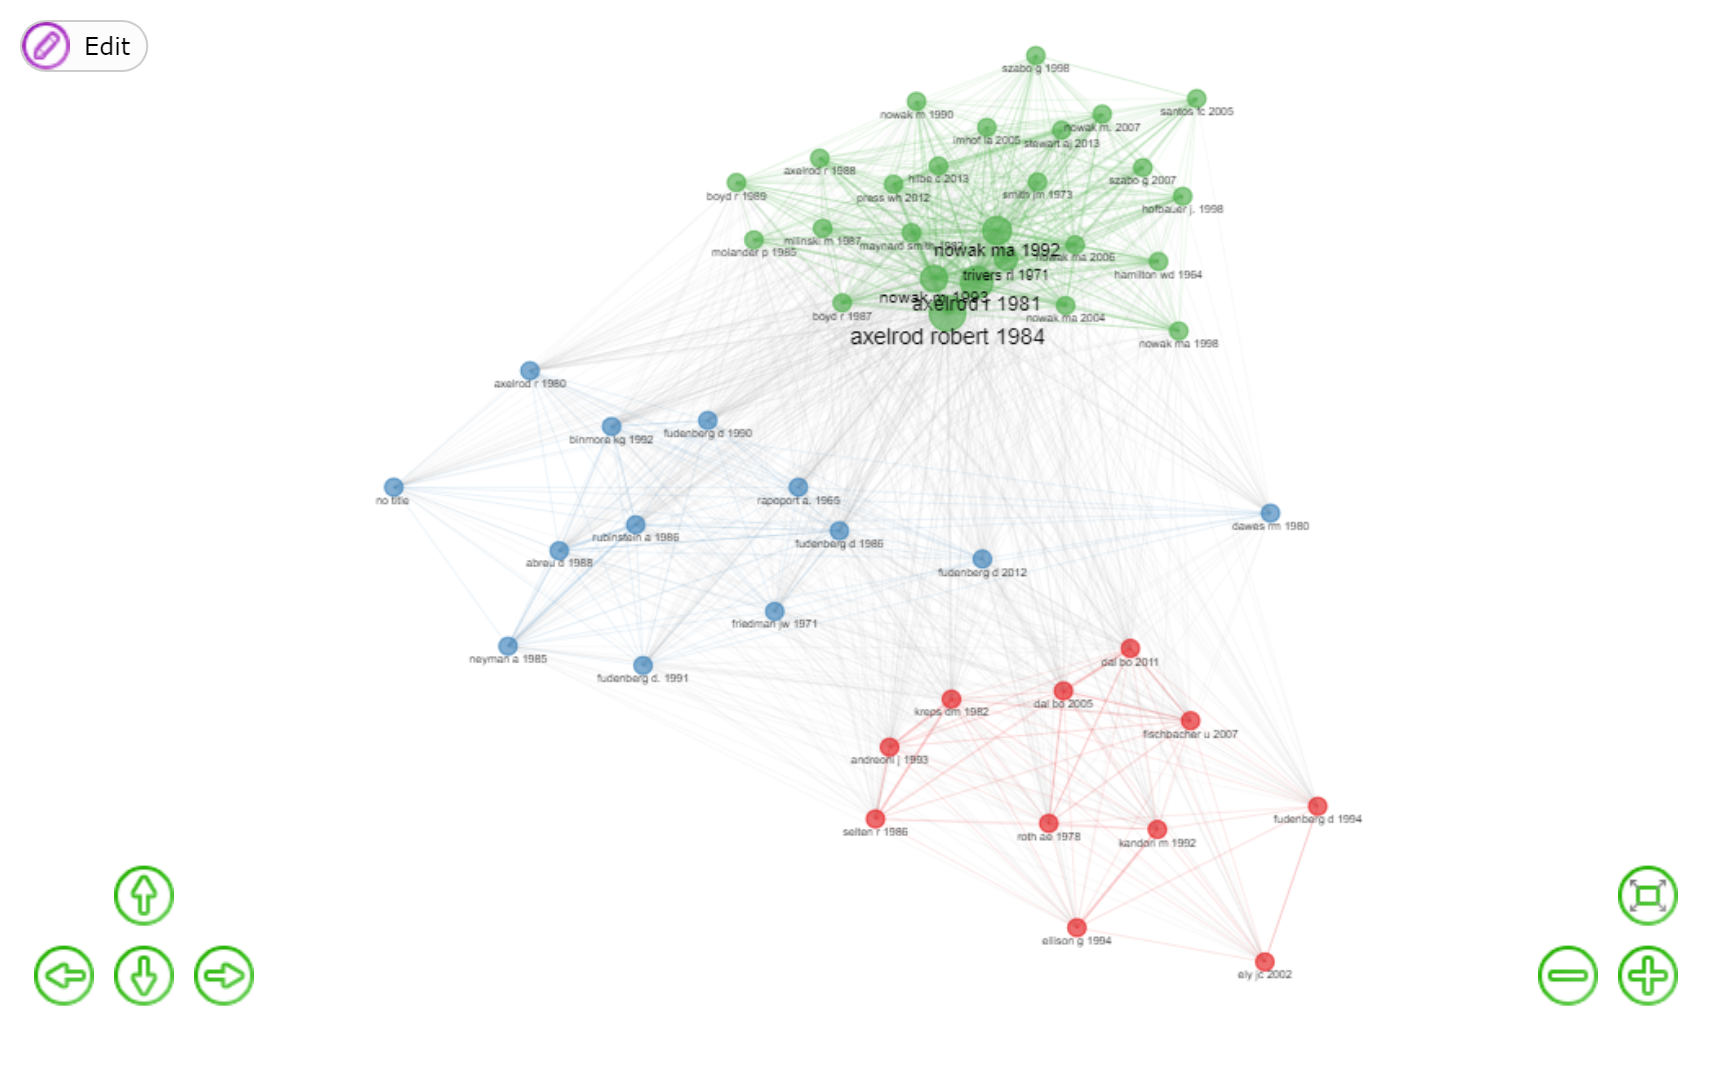
\includegraphics[width=1\textwidth]{exploratory-data-analysis/jvcalassio/PesqBibliogr/PrisonersDilemma/WoS-20221201/Dataset/Co-citation-Network-Papers-2022-12-03.png}
    \caption{Rede de co-citação entre as 50 referências mais presentes no  \dataset\ PD@jvcalassio.}
    \label{fig:PD@jvcalassio:CoCitation-Network}
\end{figure}

\subsubsection{Historiografia}

O mapa histórico das citações diretas entre os documentos mais evidentes pode ser visto na figura \ref{fig:PD@jvcalassio:HistoricalDirectCitationNetwork-50docs}.

\begin{figure}
    \centering
    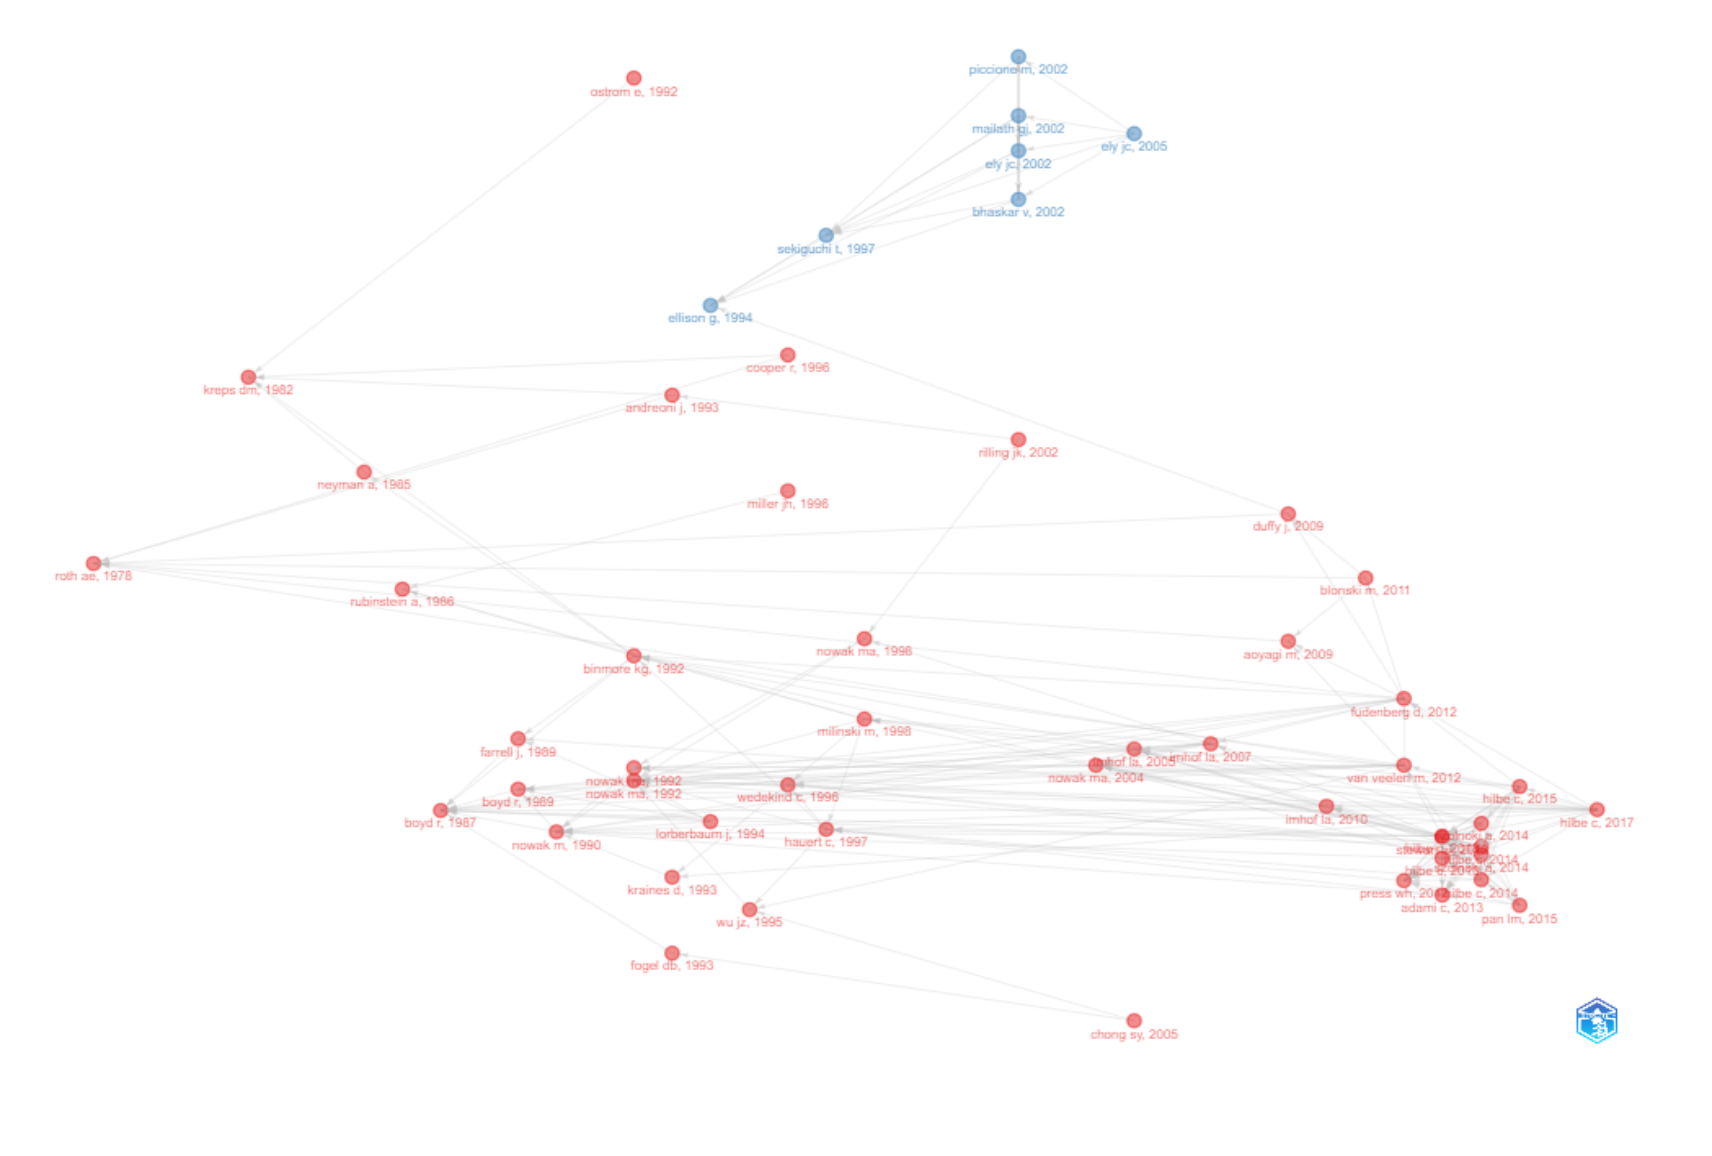
\includegraphics[width=1\textwidth]{exploratory-data-analysis/jvcalassio/PesqBibliogr/PrisonersDilemma/WoS-20221201/Dataset/Historiograph-2022-12-03.png}
    \caption{Mapa histórico das citações diretas entre os documentos mais evidentes no  \dataset\ PD@jvcalassio.}
    \label{fig:PD@jvcalassio:HistoricalDirectCitationNetwork-50docs}
\end{figure}

\subsection{Estrutura Social do Conhecimento}

Conhecimento científico é produzido socialmente, por meio de autores trabalhando em conjunto, e uma estrutura de filiações a organizações permanentes ou periódicas, que realizam ou promovem pesquisas, nelas incluídos os centros de pesquisa, universidades, departamentos, institutos, faculdades, eventos, revistas, conferências, e que evoluem ao longo do tempo. A análise da estrutura social do conhecimento evidencia esses relacionamentos, que iniciam no plano pessoal, e evoluem para outros escopos.

\subsubsection{Rede de Colaboração}

As redes de colaboração entre instituições, autores e países podem ser visualizadas nas figuras \ref{fig:PD@jvcalassio:Collaboration-Network-50instit}, \ref{fig:PD@jvcalassio:Collaboration-Network-50authors} e \ref{fig:PD@jvcalassio:Collaboration-Network-50country}, respectivamente. Podemos notar grande colaboração entre grandes potências mundiais e referências em pesquisa, como os Estados Unidos, China, Japão, Alemanha, etc. e vários pontos isolados como a Rússia e a Armênia.

\begin{figure}
    \centering
    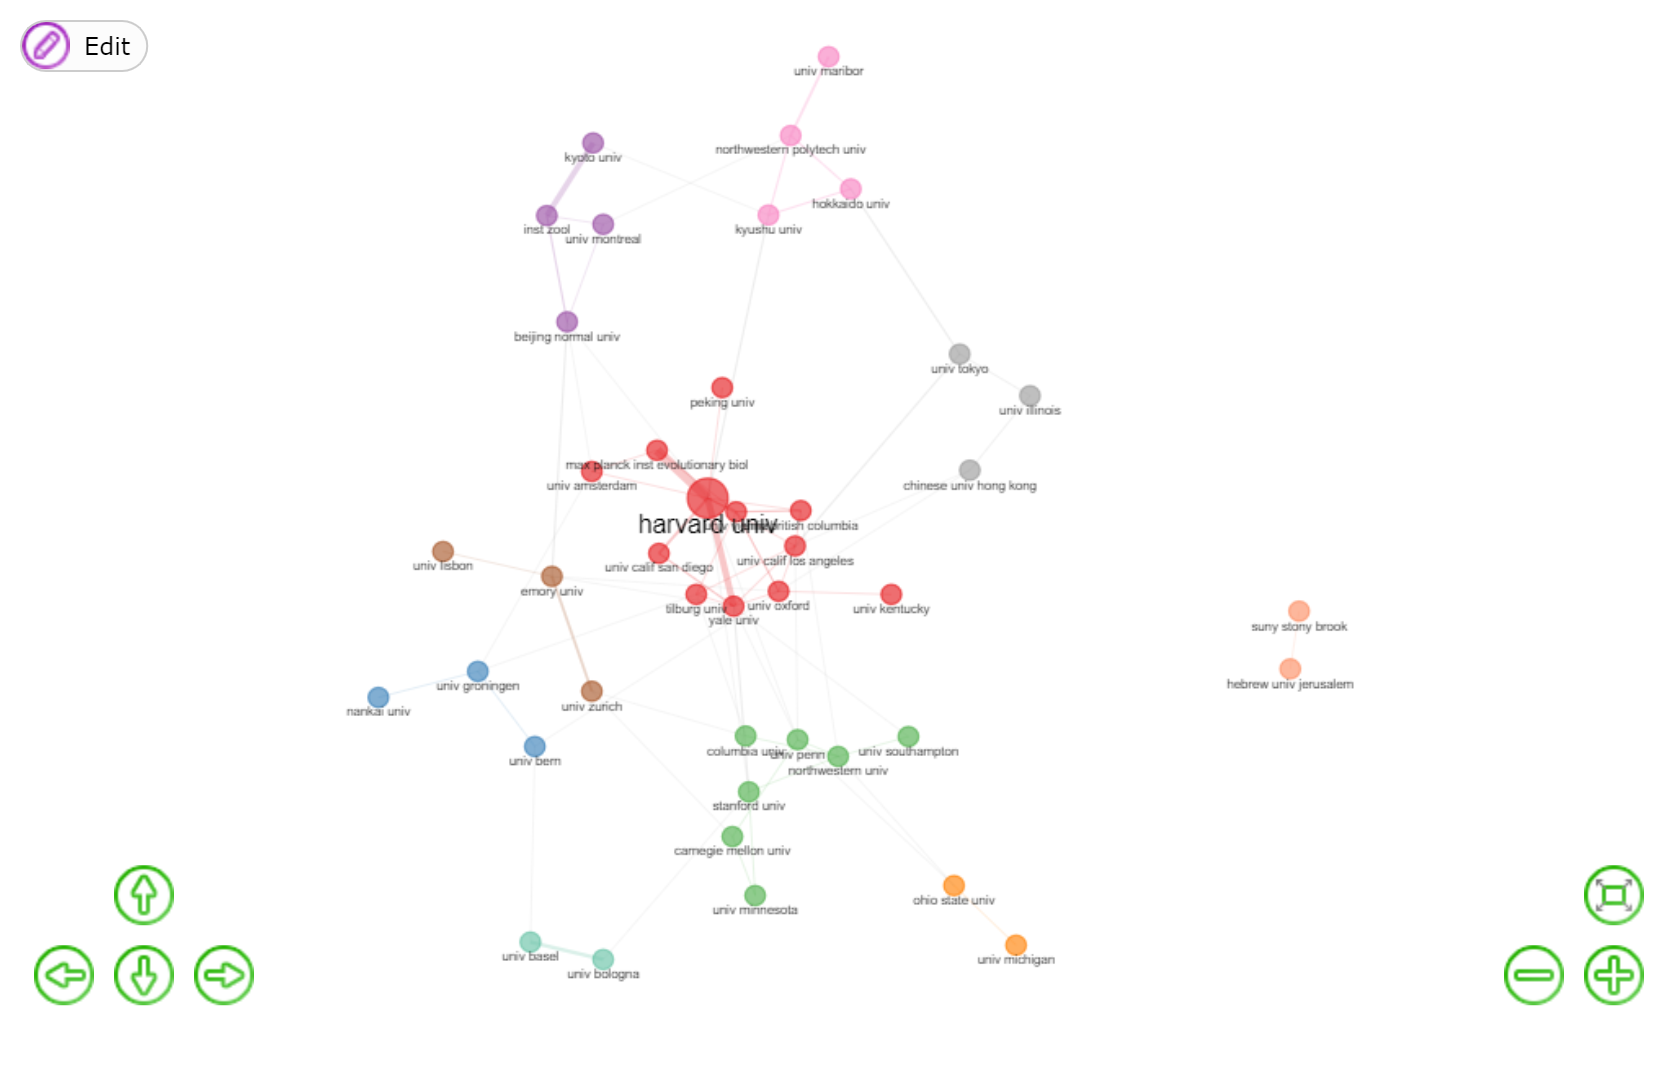
\includegraphics[width=1\textwidth]{exploratory-data-analysis/jvcalassio/PesqBibliogr/PrisonersDilemma/WoS-20221201/Dataset/Collaboration-Network-Institutions-2022-12-03.png}
    \caption{Rede de colaboração entre as 50 instituições mais evidentes, no  \dataset\ PD@jvcalassio.}
    \label{fig:PD@jvcalassio:Collaboration-Network-50instit}
\end{figure}

\begin{figure}
    \centering
    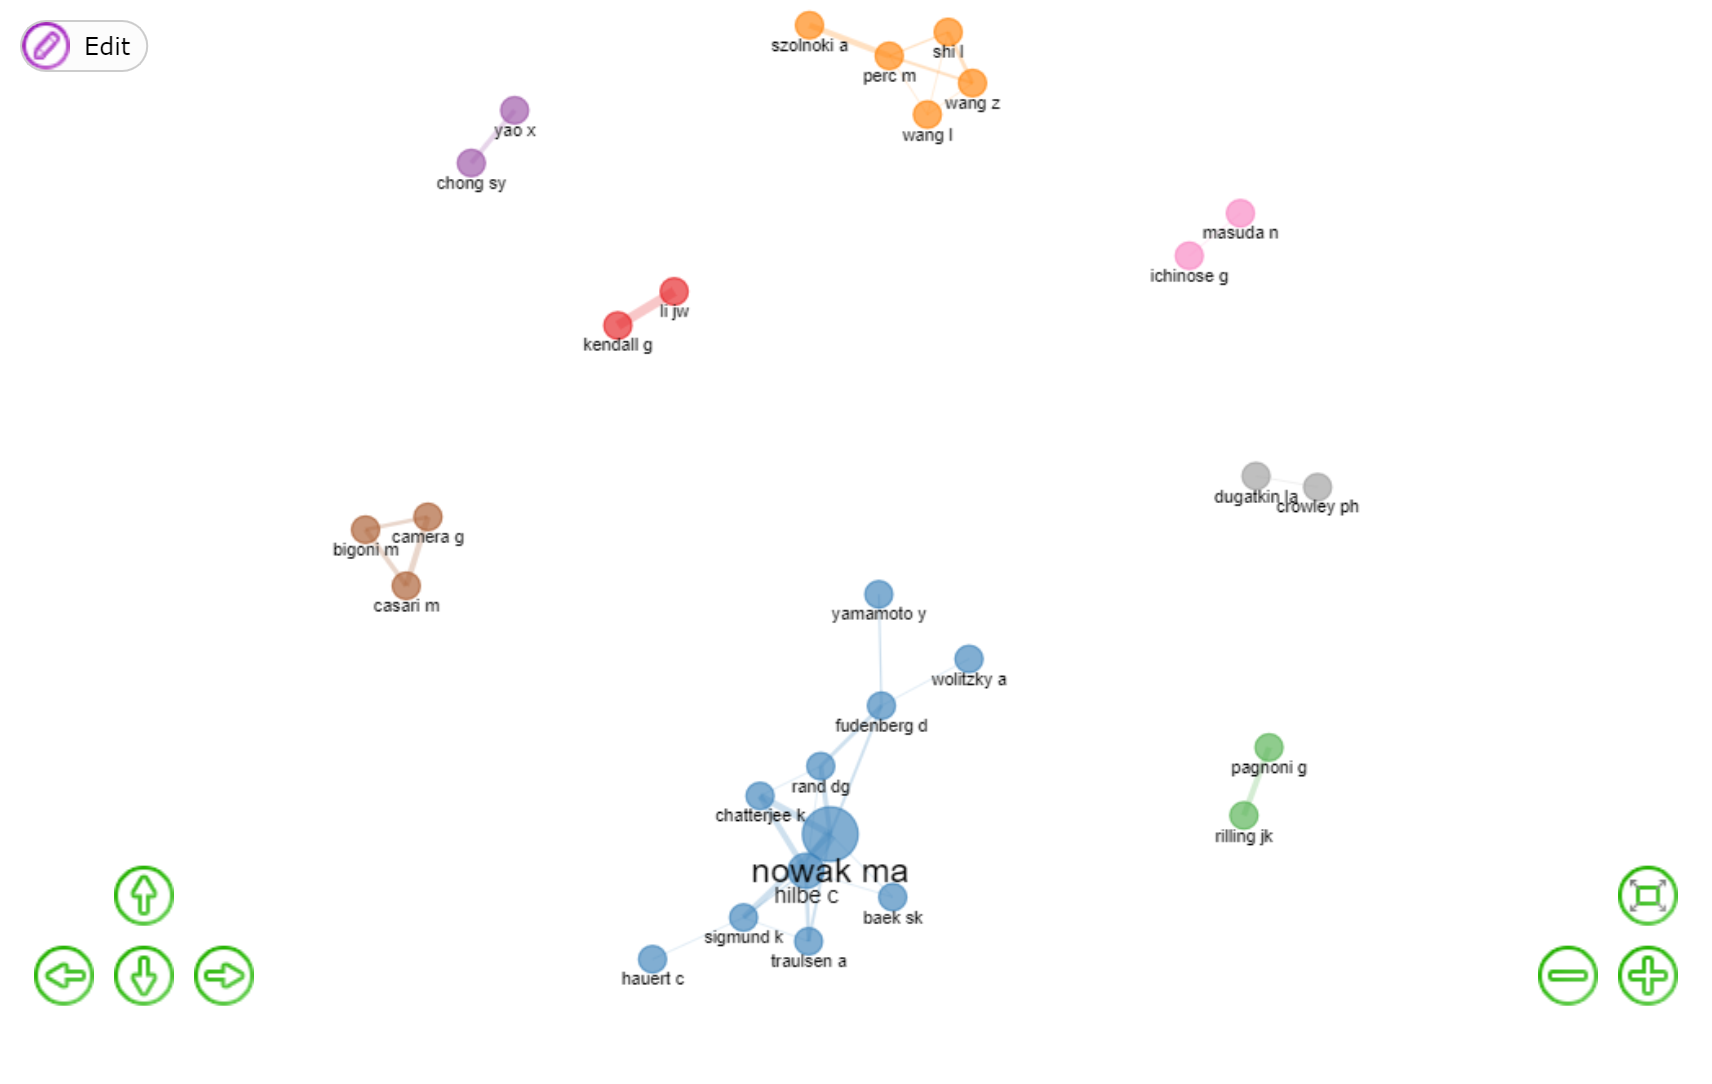
\includegraphics[width=1\textwidth]{exploratory-data-analysis/jvcalassio/PesqBibliogr/PrisonersDilemma/WoS-20221201/Dataset/Collaboration-Network-Authors-2022-12-03.png}
    \caption{Rede de colaboração entre os 50 autores mais evidentes, no  \dataset\ PD@jvcalassio.}
    \label{fig:PD@jvcalassio:Collaboration-Network-50authors}
\end{figure}

\begin{figure}
    \centering
    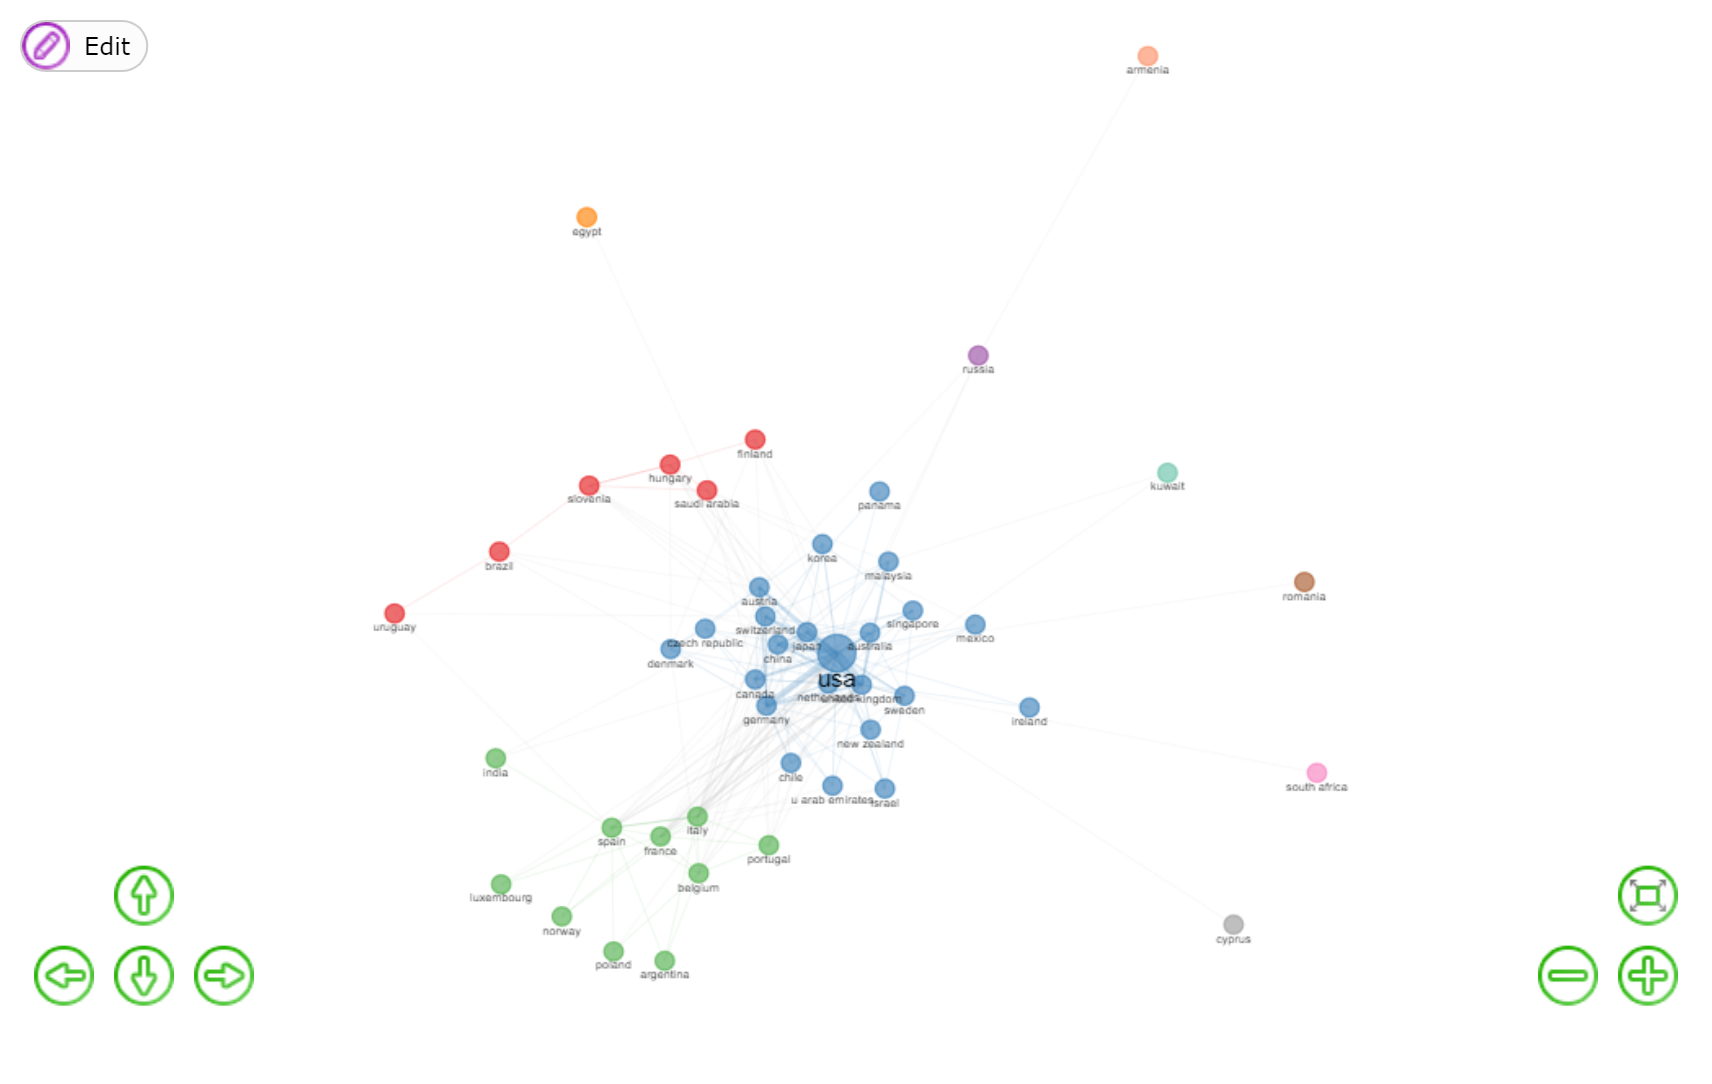
\includegraphics[width=1\textwidth]{exploratory-data-analysis/jvcalassio/PesqBibliogr/PrisonersDilemma/WoS-20221201/Dataset/Collaboration-Network-Countries-2022-12-03.png}
    \caption{Rede de colaboração entre os 50 países mais evidentes, no  \dataset\ PD@jvcalassio.}
    \label{fig:PD@jvcalassio:Collaboration-Network-50country}
\end{figure}

\section{Análises\label{PD@jvcalassio:Analises}}

Julgando pela figura \ref{fig:PD@jvcalassio:FactorialAnalysis-MCA-FactorialMap}, na página \pageref{fig:PD@jvcalassio:FactorialAnalysis-MCA-FactorialMap}, podemos imaginar que há duas grandes frentes de pesquisa no tema do dilema do prisioneiro iterativo, dado que o mapa se divide em duas grandes áreas (polígono azul e polígono vermelho). No entanto, ao analisarmos de perto quais são os termos que definem essas áreas, podemos observar que as pesquisas na área representada pelo polígono azul buscam compreender fenômenos muito semelhantes aos que estão sendo estudados também no polígono vermelho: a evolução e a estabilidade do dilema do prisioneiro, e como fenômenos como a extorsão e a generosidade afetam resultados finais. 

A área de pesquisa ilustrada pelo polígono vermelho estuda muitos outros fenômenos relacionados ao dilema do prisioneiro, como a cooperação, estratégia, punição, reciprocidade, tomada de decisão, confiança, evolução, etc., mas também voltados para entender como eles afetam a evolução e a estabilidade de iterações futuras do dilema do prisioneiro, e como isso afeta a individuos em uma sociedade.

Com relação ao uso de simulações, podemos observar que elas são amplamente utilizadas para compreender como esses fenômenos acontecem em sociedades e como ocorre a evolução das interações entre indivíduos a cada repetição. Simulações são utilizadas em \cite{axelrod_evolution_1981}, para realizar os torneios que verificam que estratégias ``olho-por-olho'' são eficientes em representar o comportamento real. Outras simulações são utilizadas em \cite{nowak_strategy_1993} para mostrar que talvez a melhor estratégia para descrever esses fenômenos seja a estratégia de \textit{Pavlov}.

\section{Conclusões}

Este trabalho está apresenta o arcabouço geral de informações que possibilitam responder às  questões formuladas no início da pesquisa, em \ref{PD@jvcalassio:questoes}:

\subsection{Base de conhecimentos}

Qual a base de conhecimentos científicos produzida em torno do tema dilema do prisioneiro iterativo, principalmente utilizando simulações? 
 
Responsa: Ver, em \ref{PD@jvcalassio:Analises} que temos um grande grupo de pesquisa voltado para entender os impactos que diferentes fenômenos como a reciprocidade e a confiança afetam a evolução de indivíduos submetidos a diversas iterações de um jogo evolucionário como o dilema do prisioneiro iterativo.

Nota-se, com base na análise da espectroscopia mais recente das referências bibliográficas do \dataset, sumarizada em \ref{fig:PD@jvcalassio:ReferenceSpectroscopy} entre os anos de 1951 e 2022, que a área parece atingir sua maturidade por volta do ano de 1992.

\subsection{Fenômenos sociais}
   
Como o dilema do prisioneiro iterativo (e simulações dele) tem sido usado para compreender fenômenos sociais? 

Resposta: Ver \ref{PD@jvcalassio:Analises}.

\subsection{Termos e conceitos centrais}

Quais os principais termos e conceitos ligados à frente de pesquisa no tema dilema do prisioneiro iterativo? 

Resposta: Ver e explorar os mapas das figuras \ref{fig:PD@jvcalassio:Co-occurrence-Network}, \ref{fig:PD@jvcalassio:ThematicMap}, entre outros.

\subsection{Estrutura Social da Comunidade}

Qual a estrutura social da comunidade, se é que existe, que pesquisa sobre o tema dilema do prisioneiro iterativo?

Resposta: Ver e analisar os mapas das figuras \ref{fig:PD@jvcalassio:Collaboration-Network-50authors}, \ref{fig:PD@jvcalassio:Collaboration-Network-50instit} e \ref{fig:PD@jvcalassio:Collaboration-Network-50country}.
